\documentclass[12pt]{report}

\usepackage{geometry}
\geometry{a4paper}

\setlength{\parindent}{2em}
\setlength{\parskip}{0em}
\usepackage{setspace}
\onehalfspacing
\AtBeginDocument{
\addtolength\abovedisplayshortskip{-0.2\baselineskip}
\addtolength\abovedisplayshortskip{-0.2\baselineskip}}
\usepackage{fancyvrb}

\usepackage{fancyhdr}
\pagestyle{fancy}
\fancyhf{}
\fancyhead[C]{\leftmark}
\fancyfoot[C]{\thepage}
\setlength{\headheight}{15pt}

\usepackage{caption}
\captionsetup[figure]{labelfont=bf,textfont=it}
\captionsetup[table]{labelfont=bf,textfont=it}

\usepackage[super,sort&compress,comma]{natbib} 
\usepackage{floatrow}
\usepackage{graphicx}
\usepackage{subfig}
\usepackage{caption}
\floatsetup[figure]{style=plain,subcapbesideposition=top}
\floatsetup[table]{style=plain,subcapbesideposition=top}
\floatsetup[table]{capposition=top}

\usepackage{stackengine}
\newcommand\xrowht[2][0]{\addstackgap[.5\dimexpr#2\relax]{\vphantom{#1}}}

\usepackage{mathtools}
\usepackage{amsmath}
\usepackage{amssymb}
\usepackage{chemformula}
\newcommand{\RomanNumeralCaps}[1]
    {\MakeUppercase{\romannumeral #1}}
\usepackage{appendix}
\usepackage{geometry}
\usepackage{lipsum}

\usepackage[intoc]{nomencl}
\makenomenclature
\setlength{\nomitemsep}{0pt}

\makeatletter
\renewcommand\thenomenclature{%
  \section*{\nomname}%
  \if@intoc\addcontentsline{toc}{section}{\nomname}\fi
  \nompreamble
  \list{}{%
    \labelwidth\nom@tempdim
    \leftmargin\labelwidth
    \advance\leftmargin\labelsep
    \itemsep\nomitemsep
    \let\makelabel\nomlabel}}
\makeatother

\setcounter{tocdepth}{1}
\title{Atomistic modelling studies of the anti-perovskite \ch{Na3OCl} sodium-ion conductor for solid-state batteries}
\author{Benedek Goldmann}

\begin{document}

\begin{titlepage}
   \begin{center}
      \vspace*{0.7 cm}
      
      {\Large\textbf{Atomistic modelling studies of the anti-perovskite \ch{Na3OCl} sodium-ion conductor for solid-state batteries} \par}

       \vspace{0.7 cm}
        
       submitted by
            
       \vspace{0.7 cm}

       {\Large\textbf{Benedek Goldmann} \par}
       
       \vspace{0.7cm}
       
       A Confirmation Report Submitted
       
       As Part of the Transfer Process to the degree of
       
       Doctor of Philosophy
       
       \vspace{0.7 cm}
       
       {\Large{University of Bath} \par}
       
       Department of Chemistry
       
       \vspace{0.7 cm}
       
       September 2021
       
       \vspace{2 cm}
       
       {\large\textbf{COPYRIGHT}}
   \end{center}
   
   \noindent   
   Attention is drawn to the fact that copyright of this report rests with the author. 
   A copy of this report has been supplied on condition that anyone who consults it is understood to recognise that its copyright rests with the author and that they must not copy it or use material from it except as permitted by law or with the consent of the author.
   
\vspace{0.7 cm}   
   
   \noindent
   Signature of Author: ..............................................................................................
\end{titlepage}

\pagenumbering{roman}

\clearpage

\tableofcontents
\thispagestyle{empty}
\clearpage





\chapter*{Abstract}
\addcontentsline{toc}{chapter}{Abstract}

Energy storage is a critical area that has come to the forefront in the battle against climate change.
With the intermittent nature of renewable sources, the efficient storage of generated energy is important for reliable, clean energy.
Solid-state batteries for energy storage applications present potential advantages over their liquid-based electrolyte equivalents, including enhanced safety and increased energy density. 
In the search for novel solid electrolytes, the anti-perovskite family of materials are attracting growing interest. 
However, while there is significant work on Li-rich anti-perovskites, their Na-based counterparts and the atomistic effects of aliovalent doping on these materials are not fully characterised. 
Here, we investigate the effects on Na-ion conductivity of doping with divalent (Mg, Ca, Sr and Ba) and trivalent cations (Al and Ga), and of possible dopant-vacancy clustering in the anti-perovskite \ch{Na3OCl} by employing atomistic simulation techniques.
Our results highlight the prospects of \ch{Mg^{2+}}, \ch{Ca^{2+}}, \ch{Al^{2+}} and \ch{Ga^{2+}} doping due to their favourable incorporation and increased Na-ion vacancy concentration. 
Local defect clustering and binding energies are analysed, and such effects inhibit Na-ion conductivity in the doped \ch{Na3OCl} solid electrolyte at operating temperatures. 
These results provide a framework to guide future work on sodium-rich anti-perovskites to enhance their solid electrolyte properties.

\clearpage





\chapter*{COVID-19 Statement}
\addcontentsline{toc}{chapter}{COVID-19 Statement}

This computational chemistry project was not affected by the lack of resources, as the high-performance computers necessary were available.
However, the government's guidance to work from home meant that working in a computational lab at the university was not possible.
Hence, most interactions with other members of the group was largely virtual.
This hindered the progress of the project somewhat, as the seeking of advice and guidance was more complicated.

\clearpage





\chapter*{Acknowledgements}
\addcontentsline{toc}{chapter}{Acknowledgements}

Firstly, I want to thank my supervisor Prof. M. Saiful Islam for the immense support throughout my first PhD. year. 
I also wish to extend my gratitude to my secondary supervisor Dr. Benjamin J. Morgan for some great advice.
Matt Clarke and Dr. James Dawson have been invaluable to both this project and my smooth transitioning into academic research in computational chemistry.

Finally, the author and supervision team are grateful to the Faraday Institution CATMAT project (EP/S003053/1, FIRG016) and the Bath URS studentship scheme for financial support, and the HEC Materials Chemistry Consortium (EP/R029431) for Archer high-performance computing facilities.

\clearpage





\chapter*{Presentations and publications}
\addcontentsline{toc}{chapter}{Presentations and publications}

{\Large\textbf{Presentations}\par}

\vspace{0.3 cm}

{\large\textbf{Oral}\par}

Dept. of Chemistry PhD Talks, Bath - February, 2021

CSCT Summer Showcase, Bath - July, 2021

\vspace{0.3 cm}

{\large\textbf{Posters}\par}

CSCT Summer Showcase, Bath - July, 2021

Bolland Symposium, Bath - September, 2021

\vspace{1 cm}

\noindent
{\Large\textbf{Publications}\par}

\vspace{0.3 cm}

\noindent
B. A. Goldmann, M. J. Clarke, J. A. Dawson and M. S. Islam, "Atomic-scale investigation of cation doping and defect clustering in the anti-perovskite \ch{Na3OCl} sodium-ion conductor", \textit{Journal of Materials Chemistry A}, 2021.

\clearpage

\noindent
{\Large\textbf{Nomenclature}}

\vspace{0.3 cm}

\noindent
Unless noted otherwise, the abbreviations listed below are used throughout the report. Bold symbols are used to represent vector quantities.

\vspace{-1.2cm}
\begin{singlespacing}
\renewcommand{\nomname}{}
\printnomenclature
\end{singlespacing}
\addcontentsline{toc}{chapter}{Nomenclature}
\thispagestyle{plain}

\nomenclature{\(\sigma\)}{Ionic conductivity}
\nomenclature{\(q\)}{Charge of a species}
\nomenclature{\(n\)}{Concentration of a species}
\nomenclature{\(\mu\)}{Mobility of a species}
\nomenclature{\(k_B\)}{Boltzmann constant}
\nomenclature{\(T\)}{Temperature}
\nomenclature{\(U\)}{Internal energy}
\nomenclature{\(U_{ij...}\)}{Potential energy of ionic interactions}
\nomenclature{\(r_{ij...}\)}{Distance between ions}
\nomenclature{\(\epsilon_0\)}{Vacuum permittivity}
\nomenclature{\(\alpha\)}{Point polarizability}
\nomenclature{\(E\)}{Size of electric field}
\nomenclature{\(\mathrm{f}\)}{Force acting on a species}
\nomenclature{\(m\)}{Mass}
\nomenclature{\(q\)}{Charge of a species}
\nomenclature{\(\mathrm{a}\)}{Acceleration}
\nomenclature{\(\mathrm{v}\)}{Velocity}
\nomenclature{\(\mathrm{r}\)}{Position of a species}
\nomenclature{\(t\)}{Time}
\nomenclature{\(\mathrm{b}\)}{Jerk}
\nomenclature{\(\Theta\)}{Error}
\nomenclature{\(N\)}{Number of species}
\nomenclature{\(\mathrm{x}_p\)}{Set of coordinates at step $p$}
\nomenclature{\(D\)}{Diffusion coefficient}
\nomenclature{\(E_a\)}{Activation energy}
\nomenclature{\(\mathrm{g}_p\)}{Gradient vector at step $p$}
\nomenclature{\(\mathrm{d}_p\)}{Search vector at step $p$}
\nomenclature{\(\mathrm{H}_p\)}{Hessian matrix at step $p$}


\clearpage





\chapter{Introduction}

\pagenumbering{arabic}

\section{Rechargeable batteries}

With increasing environmental concerns surrounding fossil fuels, it has become abundantly clear that a shift towards renewable energy generation is necessary.\cite{chu2017, chu2012}
There is also a need for suitable energy storage systems to overcome issues related to the intermittency of such technologies. 
Rechargeable batteries may be able to offer a reliable solution to this challenge.\cite{islam2014, liu2013, dunn2011, goodenough2010, armand2008}

Rechargeable batteries consists of oppositely charged electrodes, known as anode (negative) and cathode (positive), separated by an electrolyte material.
For the Li-ion battery, the anode is normally composed of graphite, while the cathode is made of a crystalline material, often \ch{LiCoO2}, as shown in Figure \ref{battery}.
The electrolyte is typically a non-aqueous liquid with a high ionic conductivity and low electronic conductivity, such as \ch{LiPF6}.
During charging, an external electric potential is applied to move electrons from the cathode to the anode, which also forces the mobile cations (commonly \ch{Li+} or \ch{Na+}) to move to the anode through the electrolyte material.
In this state, the battery can store energy for extended periods of time as electrochemical potential energy.
As the battery discharges, both the electrons and the cations move back to the cathode along the electrochemical gradient.
Electrons take an external path doing electric work, providing electricity, while cations move back through the electrolyte material.\cite{islam2014}

\begin{figure}[!ht]
\centering
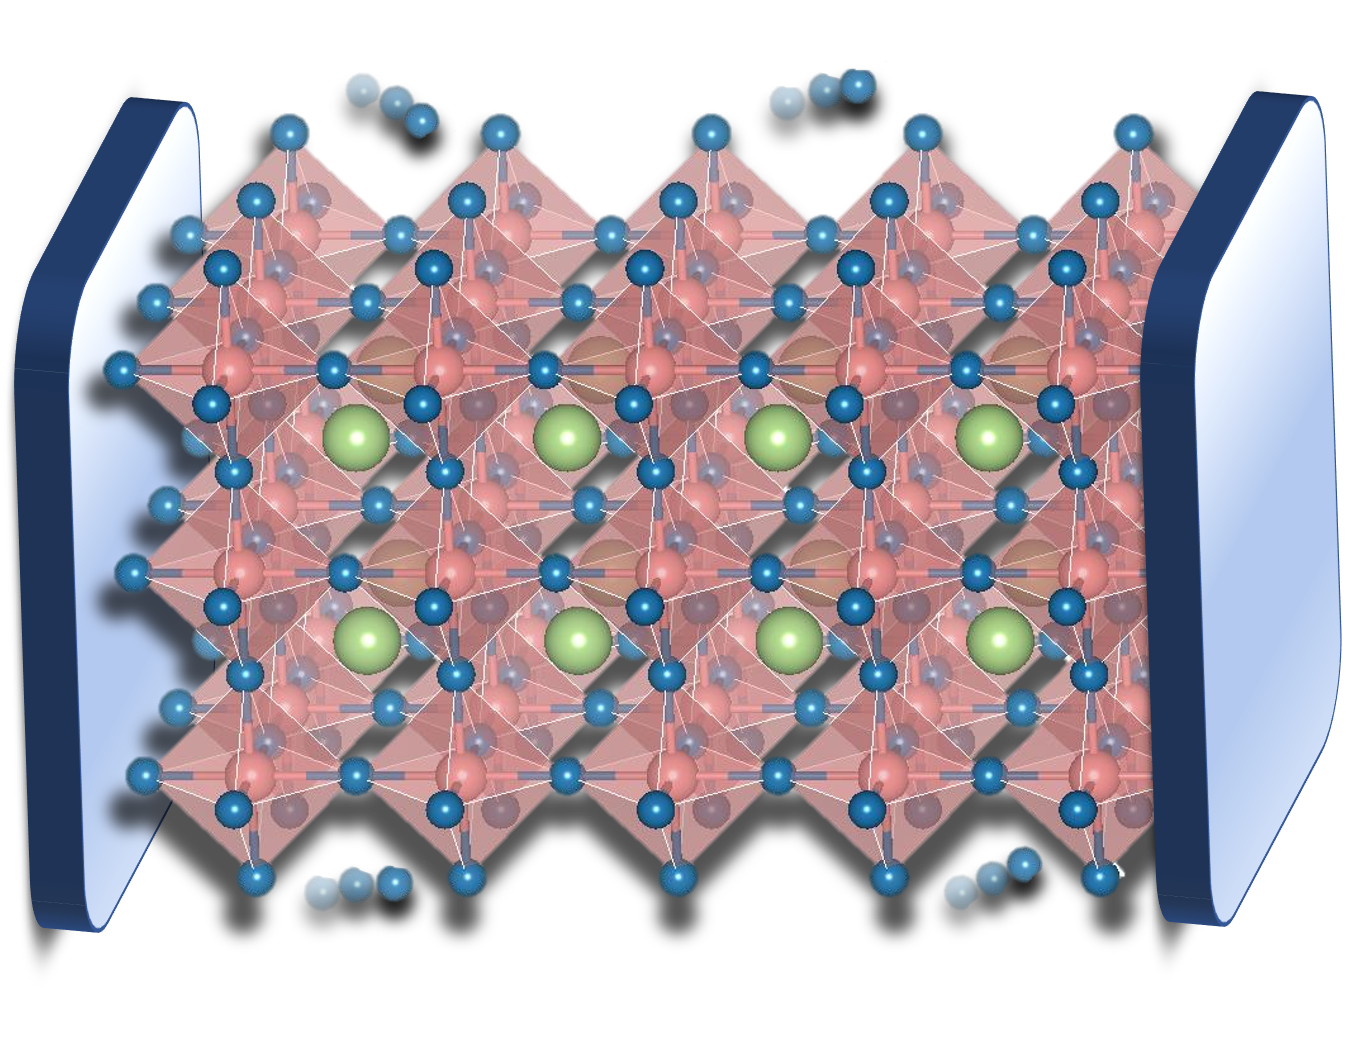
\includegraphics[width=8 cm]{./figures/battery.png}
\caption{Schematic of a rechargeable battery during discharge.\cite{islam2014}}
\label{battery}
\end{figure}


\section{Solid-state batteries}

\subsection{Advantages of solid electrolytes}

Conventional rechargeable batteries employing liquid electrolytes have been the focal point for research relating to energy storage for the past two centuries. 
The use of liquid electrolytes has many advantages including high conductivity and excellent wetting of the electrode surfaces. 
However, liquid electrolytes are highly flammable and show poor thermal and electrochemical stability which lead to safety issues as well as low cyclability.\cite{goodenough2012}

Solid electrolytes (SEs) used in solid-state batteries are an alternative attracting growing interest.\cite{famprikis2019, zhang2018b, ohno2020, bachman2016, manthiram2017, gao2018, kim2017,zhao2018, dawson2018b} 
The use of solid electrolytes allows for the elimination of flammable, thermally unstable liquids resulting in much safer batteries that can be operated at a wider temperature ranges.
Furthermore, the introduction of the solid electrolyte reduces the dynamic nature of the electrolyte-electrode interface, meaning the transition metals in the cathode do not significantly dissolve or react with the electrolyte.
This results in better cyclability, which is more economic and sustainable.

Another advantage of solid electrolytes is their compatibility with metallic anodes.
Changing the anode of a battery from graphite to Li metal would lead to its energy density being increased by over 20\%.\cite{janek2016}
However, liquid electrolytes are incompatible with Li anodes due to the growth of needle-like projections, known as dendrites, forming at the anode surface, growing across the electrolyte and leading to reduced cyclability, even short-circuiting.
This effect is considerably suppressed with the use of solid electrolytes, although it has recently been shown that the strings of Li metal can in fact penetrate solid electrolytes, too.\cite{porz2017}
Nevertheless, if a solid-state battery with Li metal anodes could be produced relatively cheaply, it would be a prime candidate to be used in electric vehicles, which many car manufacturers are developing (see Figure \ref{tesla}).\cite{luntz2015}

\begin{figure}
    \centering
    
\includegraphics[width=10cm]{figures/tesla.jpeg}
    \caption{Solid-state lithium batteries with metallic lithium anodes are prime candidates to be used in electric vehicles, such as this Tesla Model X, due to their high energy density.}
    \label{tesla}
\end{figure}

\subsection{Ionic transport in solid electrolytes}

Ionic transport in solid electrolytes is a multiscale process, with a range of mechanisms operating over different scales. 
The overall ionic conductivity in a solid is a function of all these mechanisms, so optimisation at every level is essential for peak solid electrolyte performance.\cite{famprikis2019} 

The lowest scale of these is the atomic scale, where mobile cations diffuse along favourable migration pathways between potential wells in the lattice. 
Examples include vacancy and interstitial migrations mechanisms. (See Appendix A)
The atomic-scale conductivity in solid materials is a thermally activated process and can be described using the expression below:

\begin{equation}
    \sigma = q n \mu
\end{equation}

\noindent
Where $n$, $ \mu $ and $q$ represent the concentration, mobility and charge of the mobile ions, respectively, with: 

\begin{equation}
    \mu \propto \exp(-E_a/k_BT)
\end{equation}

\noindent


Groups of ions arranged in a specific pattern make up a local environment on the microscopic scale.
The bulk crystal, inhomogeneities such as grain boundaries, and amorphous regions are all examples of such environments. 

Going another level up is the macroscopic scale, which encompasses collections of microscopic environments.
This is typically the scale where conductivity can be directly measured in experiments.
Therefore, the experimental conductivity of a solid is dependent on all the different microscopic environments it is composed of and hence can vary between samples.

Lastly is the device scale, which includes the electrolyte material, the electrodes and the interactions between these materials.
It is important to note that drawing a link between the conductivity on the macroscopic and device scale is not trivial, as the compatibility of the different materials used is critical.\cite{famprikis2019} 
The focus of this work is primarily optimization on the atomic scale, but the microscopic, macroscopic and device environments are also touched upon. 

\begin{figure}[!ht]
\centering
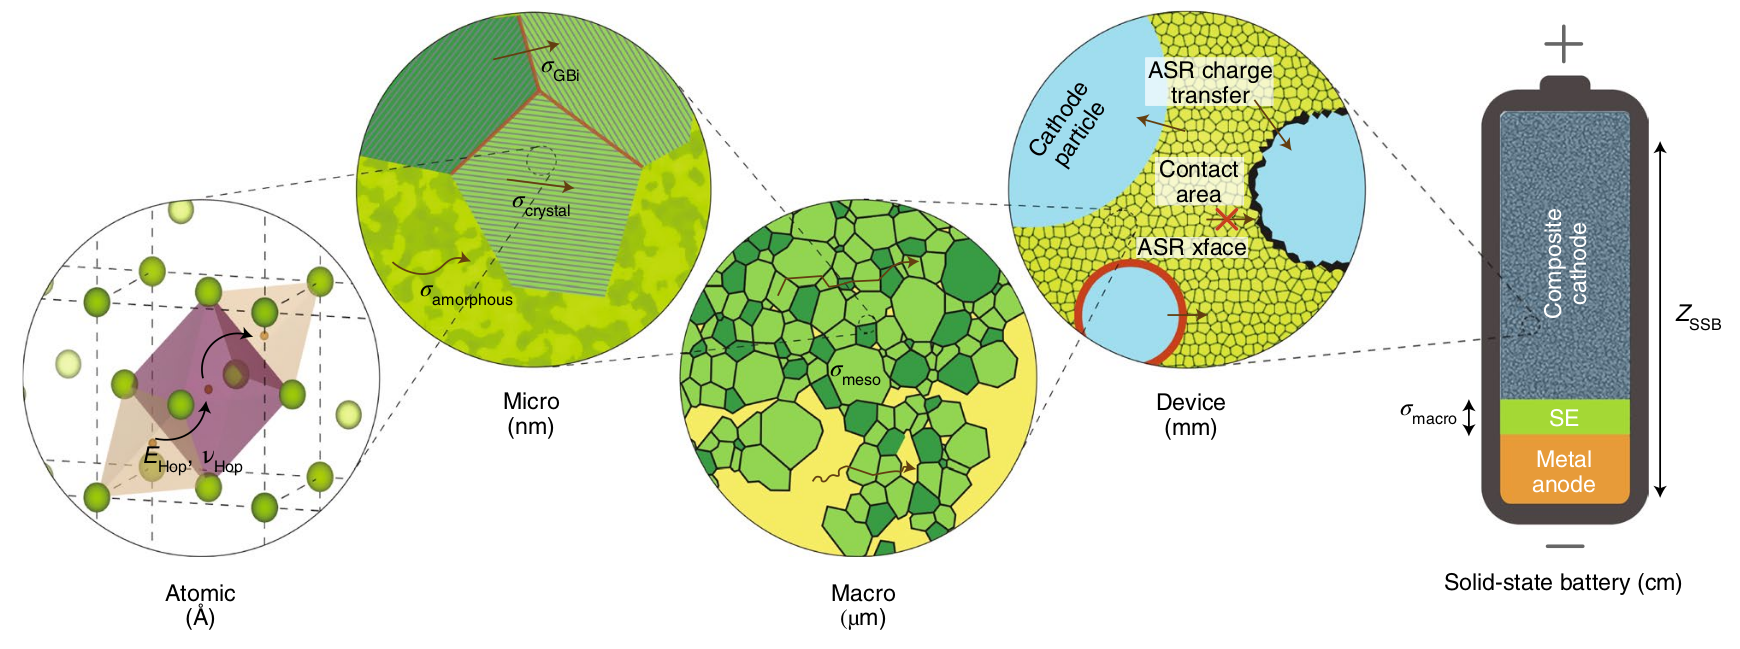
\includegraphics[width=\textwidth]{./figures/scales.png}
\caption{Schematic of the multiscale ion transport in solids. The illustrations highlight the major descriptors related to ionic transport at each scale. These include the energy and frequency of ionic hops ($E_{Hop}, \ \nu_{Hop}$) at the atomic scale, the conductivities ($\sigma$) at the micro- and macroscopic scale, the area-specific resistances ($ASR$) at the device scale and finally the total device impedance ($Z_{SSB}$).  \cite{famprikis2019}}
\label{scales}
\end{figure}

\subsection{Improving solid electrolytes}

The use of solid electrolytes has several benefits, however, this technology currently suffers from three major limitations that prevent the wide-spread commercialisation of solid-state batteries. 
Firstly, the bulk ionic conductivity of solid electrolytes on the atomic scale is significantly lower than that of their liquid-based equivalents.
This is a direct consequence of the energetic difference between ions diffusing along a relatively smooth electrochemical gradient in liquid environments compared to a hopping mechanism with activation barriers in solids.
Secondly, the presence of inhomogeneities, such as grain boundaries, creates further barriers for ionic migration on a macroscopic scale, often leading to the overestimation of ionic conductivity in theoretical studies.
Finally, the movement of ions across the SE-electrode interfaces is often inefficient, primarily due to contact issues, which hinders ionic migration on the device scale.

The latter two limitations can be addressed by the optimisation of production, starting with synthesis and densification of the solid electrolyte, followed by its integration into the solid-state battery.

The most direct synthetic route involves mixing the reagents thoroughly, then annealing the mixture at high temperatures.
While this method is simple, it is energy intensive, may produce harmful gaseous by-products and may damage the equipment.
An alternative is soft chemistry, where reagents are mixed in the presence of a solvent, which reduces the energy requirements and is more favourable for scalability if  solvents are effectively recycled.
A third method is mechanochemical synthesis (typically ball-milling) which relies on the high-energy impact between solid particles to achieve a favourable reaction environment.
This allows the reaction to proceed at lower temperatures, however, the safety and energy-efficiency of the method is still unclear.

The next step in the processing is the densification of the synthesised electrolyte, which is necessary to achieve high-aspect-ratio membranes or pellets.
The desired microstructure can be achieved though sintering followed by either cold or hot pressing of the dry powders.
Spark plasma sintering (SPS) is an attractive alternative for densification, as it allows for the precise control of the microstructure to ensure optimal ionic conductivity.
However, this method is far too costly to be used on an industrial scale.

The industrialized method for the integration of solid electrolytes into solid-state microbatteries are based on thin-films.
Although these achieve excellent solid-solid contact to minimize the interfacial impedance, it is uncertain whether it can be scaled up to bulk solid-state battery production.
Another route for integration is the simple cold pressing of components, however, there are concerns regarding impedance on the device scale.\cite{famprikis2019}
The range of variables at each step of production means that finding the optimal conditions for different types of solid electrolytes is a challenge and while there is a vast amount of research directed at this area,\cite{he2021} they are largely beyond the scope of this work.

Instead, the primary focus of this report is the optimization of bulk conductivity of potential solid electrolyte materials on the atomic scale.
This is done by manipulating the crystal structure to improve atomic scale migration by increasing (i) the ionic mobility, $\mu$ or (ii) the concentration of charge carriers, n.
There are two successful strategies employed to increase atomic scale ionic conductivity in such manner: iso- and aliovalent doping.

Isovalent doping involves the introduction of large, polarizable ions to the structure to expand the lattice, reduce the activation energy for ionic hops and hence increase $\mu$.
While wider channels are usually desirable, there is a point at which increasing the channel size further is counter-productive and leads to a loss of the specific geometry required for the ion migration.
Therefore, it is important to find the optimal channel size for maximized conductivity.
Isovalent dopants displace an ion of the same valency and do not induce any other defects.

Even with ideal channels for ionic migration, perfect crystals tend to be poor ionic conductors, and disorder in the structure is vital for the migration of mobile charge carriers through solids.
Increasing the defect concentration in the lattice can increase ionic conductivity by enabling ionic motion and hence effectively increasing the concentration of charge carriers, n.
Aliovalent dopants have different valency than the displaced ions and therefore induce potentially useful defects when introduced, to conserve the overall charge of the structure.
To make sure aliovalent doping leads to an increase in conductivity, it is important to understand the mechanism of charge carrier transport, and dope the material accordingly.\cite{bachman2016} (See Appendix A)

\section{Sodium-based solid electrolytes}

Li-ion batteries have enabled the portable electronics revolution over the past few decades, thanks to the superior energy density they can provide.\cite{goodenough2013, thackeray2012} 
However, the demand for Li-ion batteries is as high as ever and lithium sources are being depleted at a rapid rate.

A promising alternative for this purpose are Na-ion solid-state batteries and Na-based solid electrolytes.\cite{zhang2018b, zhao2018, kim2017, ren2017, guin2015, islam2014, ellis2012}
Sodium's abundance in the Earth's crust is 23,600 ppm, compared to just 20 ppm for lithium. \cite{haynes2016} 
This gives sodium-based technologies a great advantage, as it allows production to be inexpensive and more sustainable.
The volume of work focused on Na-based solid electrolytes is rapidly increasing, with the most promising groups being oxide- and sulphide-based materials.

\subsection{Oxide-based materials}

Inorganic conductors with mobile \ch{Na+} charge carriers, such as \ch{Na-$\beta/\beta$’’-Al2O3}, have been known for over half a century.
In fact, it was the emergence of the \ch{Na-$\beta$''-Al2O3} structure that allowed the commercialisation of the first system with a solid electrolyte, the high-temperature Na/S battery.\cite{yao1967}
However, the extremely high sintering temperatures needed for production limits the practical application of these early Na-based solid electrolytes. \cite{hueso2013}

\begin{figure}[h!]
\centering
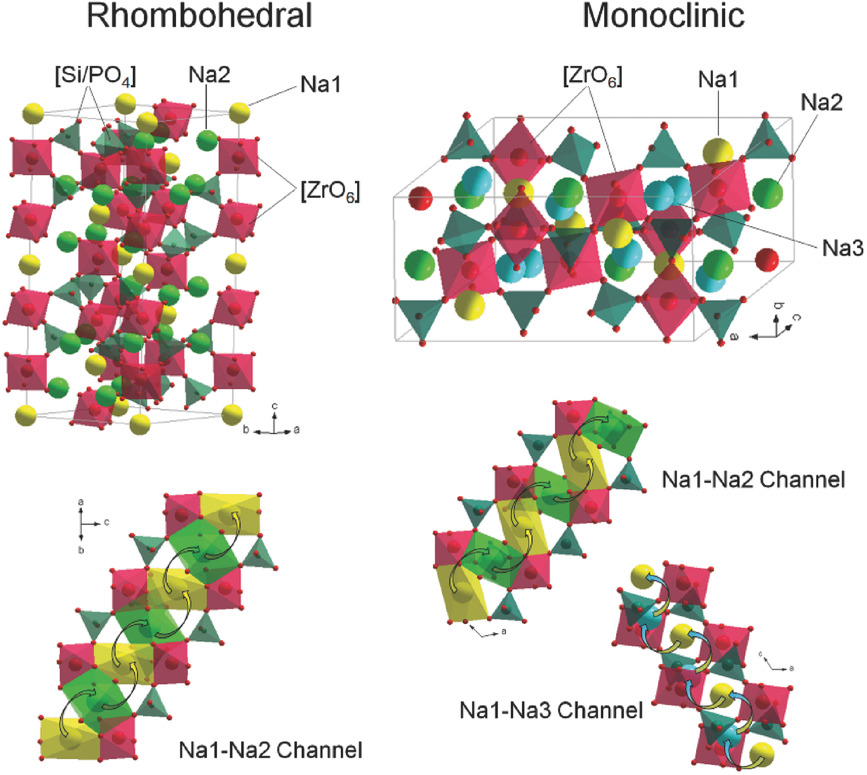
\includegraphics[width=12cm]{./figures/nasicon.jpg}
\caption{Crystal structures of the two phases of the \ch{Na3Zr2Si2PO12} NASICON compound and the ionic transport paths within them. \ch{Zr^{4+}} ions and \ch{ZrO6} octahedra are shown in red, while \ch{Si^{4+}/P^{5+}} ions and \ch{Si/PO4} tetrahedra are coloured turquoise. The small red spheres represent oxide ions. The different Na ion environments are shown as yellow, green and blue spheres with their coordination environment given the same colour. \cite{zhao2018}}
\label{nasicon}
\end{figure}

The NASICON family of materials are currently the most promising oxide-based sodium-ion conductors.\cite{goodenough1976, hong1976}
This group of materials is described by the general formula \ch{Na_{1+$x$}Zr2Si_{$x$}P_{$3-x$}O12} $(0 \leq x \leq 3)$ and can form two phases of rhombohedral (high T) and monoclinic (low T), as shown in Figure \ref{nasicon}. 
In both phases the Na-ion migration takes place along the \ch{SiO4}/\ch{PO4} tetrahedra and the \ch{ZrO6} octahedra as shown in Figure \ref{nasicon}.
For the structure with $x = 2$, conductivities of up to $6.7 \times 10^{-4} \, \mathrm{S \, cm^{-1}}$ could be obtained at room temperature.\cite{goodenough1976}

The open framework of NASICONs allows for a wide range of potential iso- and aliovalent dopants to be incorporated on both the Si/P site (\ch{Ge^{4+} \ or \ As^{4+}}) and the Zr site (divalent \ch{Mg^{2+}, \ Co^{2+} \ and \ Zn^{2+}; \ trivalent \ Y^{3+} \ and \ Sc^{3+}; \ tetravalent \ Ti^{4+}, \ Sn^{4+} \ and \ Hf^{4+}; \ pentavalent \ V^{5+}, \ Nb^{5+} \ and \ Ta^{5+}}).
However, doping on the Zr site often leads to the formation of a glassy phase, which can cause problems due to its high electronic conductivity.\cite{anantharamulu2011, kreuer1989, vogel1984, ma2016, krok1989, takahashi1980, guin2015}

The best performing suphide-based structures for electrolyte applications are \ch{Na_{3.4}Sc_{0.4}Zr_{1.6}Si_{2}PO12} and \ch{Na_{3.2}Hf2(SiO4)_{2.2}(PO4)_{0.8}} with reported ionic conductivities of $4.0 \times 10^{-3} \, \mathrm{S \, cm^{-1}}$ and $2.3 \times 10^{-3} \, \mathrm{S \, cm^{-1}}$ at room temperatures, respectively.
Although doping with expensive metals like Sc and Hf is not sustainable for practical applications, the high ionic conductivities reported highlight the potential of this family of materials.\cite{ma2016, vogel1984}

\subsection{Sulphide-based materials}

Sulphide ions are larger and more polarizable than oxides, so the activation energy for ionic migration tends to be lower in sulphide-based materials than in their oxide analogues. \cite{cao2014}
Sodium thiophosphates are the most well-known from this group of materials, with \ch{Na3PS4} attracting the most attention due to its high ionic conductivity.
While the structure exists in two phases of cubic and tetragonal (Figure \ref{ngps}), it is important to note that in fact both of them exhibit the same tetragonal motif on a local scale.\cite{krauskopf2018}
The cubic phase shows a higher conductivity of $2.0 \times 10^{-4} \, \mathrm{S \ cm^{-1}}$ at room temperature.\cite{hayashi2012, famprikis2020}

Theoretical studies showed that the perfect \ch{Na3PS4} shows low conductivities, and much of the superionic properties found experimentally are attributed to defects.
It then follows that iso- and aliovalent doping are both effective strategies to increase conductivity in the \ch{Na3PS4} structure.
Partial or complete isovalent substitution with \ch{Se^{2-}} for \ch{S^{2-}} or \ch{Sb^{5+}}/\ch{As^{5+}} for \ch{P^{5+}} has been investigated with \ch{Na3SbS4} and \ch{Na3SbSe4} reported  at $3 \times 10^{-3} \, \mathrm{S \ cm^{-1}}$ and $3.7 \times 10^{-3} \, \mathrm{S \ cm^{-1}}$. \cite{wang2016, yu2017, zhang2015, banerjee2016, bo2016, zhang2016, wang2018}
Aliovalent doping to increase Na vacancy concentration can also lead to improvements: doping with \ch{Si^{4+}} for \ch{P^{5+}} in the cubic phase can improve conductivity up to $7.4 \times 10^{-4} \, \mathrm{S \ cm^{-1}}$, while partial substitution of \ch{Cl-} for \ch{S^{2-}}  in the tetragonal phase can yield a conductivity of $1.0 \times 10^{-3} \, \mathrm{S \ cm^{-1}}$.\cite{tanibata2014, chu2016,zhu2015}
Combining the two doping strategies, the sodium-ion conductor \ch{Na_{2.88}Sb_{0.88}W_{0.12}S_4} displays a conductivity of 3.2 $\times 10^{-2} \ \mathrm{S cm^{-1}}$, which is higher than the benchmark electrolyte \ch{Li10GeP2S12}.\cite{hayashi2019}

\begin{figure}[!ht]
\centering
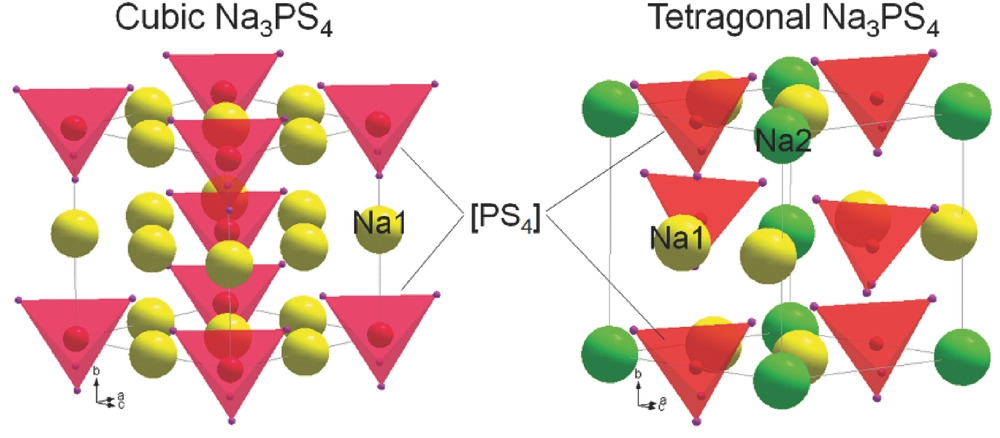
\includegraphics[width=12cm]{./figures/ngps.jpg}
\caption{Crystal structure of the cubic and tetragonal phases of \ch{Na3PS4}. \ch{P^{5+}} ions and \ch{PS4} tetrahedra are shown in red. The small red spheres represent sulphide ions. The different Na ion environments are shown as yellow and green spheres.\cite{zhao2018}}
\label{ngps}
\end{figure}

Another group of suphide-based electrolytes that recently gathered interest is the Na version of LGPS materials, although much of phase stability and conductivity mechanisms is
still unknown.\cite{kandagal2015}
\ch{Na10SnP2S12} was synthesised with a proposed structure made of chains of \ch{NaS4} tetrahedra  providing migration paths, allowing for a Na-ion conductivity of $4 \times 10^{-4} \ \mathrm{S \ cm^{-1}}$.\cite{richards2016}
Later a material with composition \ch{Na11Sn2PS12} was reported with a high degree of disorder and a 3D Na-ion conductivity of $1.4 \times 10^{-3} \ \mathrm{S \ cm^{-1}}$.\cite{zhang2018c}

\subsection{Anti-perovskite materials}

The anti-perovskite crystal structure shown in Figure \ref{fig:distortions_1} consists of divalent anions at the typical B-site of an \ch{ABX3} perovskite, coordinated to six \ch{Li+ / Na+} ions at the X-site, and monovalent anions occupying the 12-coordinate A-site.
The ideal anti-perovskite is cubic and belongs to space group 221 (Pm$\overline{3}$m), but tetragonal, orthorhombic, rhombohedral and hexagonal phases have also been reported.\cite{megaw1946, bhalla2000}
Anti-perovskites present several features that make them useful as solid electrolytes, including high ionic conductivity, negligible electronic conductivity, wide electrochemical windows and soft mechanical properties. 
Another favourable aspect of these materials is their flexible crystal structures, which allows the tailoring of mechanical and ion transport properties through doping.\cite{dawson2021, wang2020b}

\begin{figure}[!ht]
\centering
    \subfloat[]{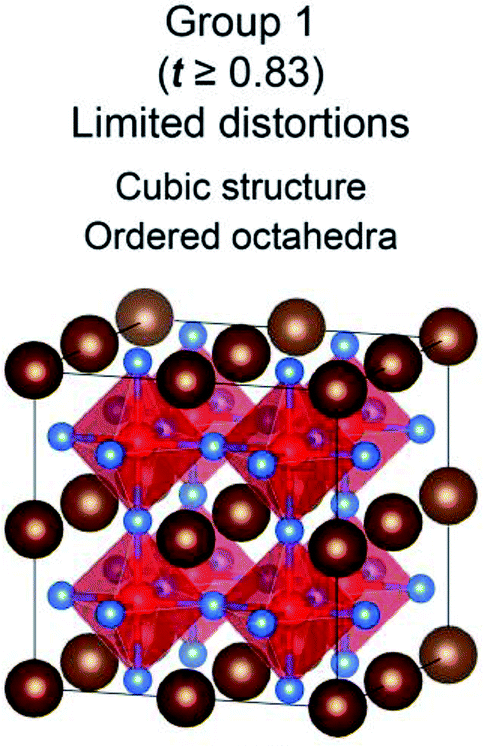
\includegraphics[height=6.5cm]{./figures/distortions_1.png}\label{fig:distortions_1}}
    \subfloat[]{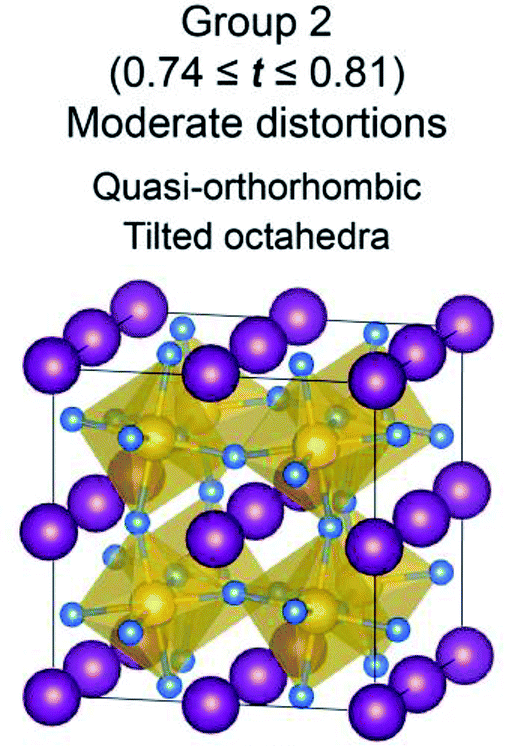
\includegraphics[height=6.5cm]{./figures/distortions_2.png}\label{fig:distortions_2}}
    \subfloat[]{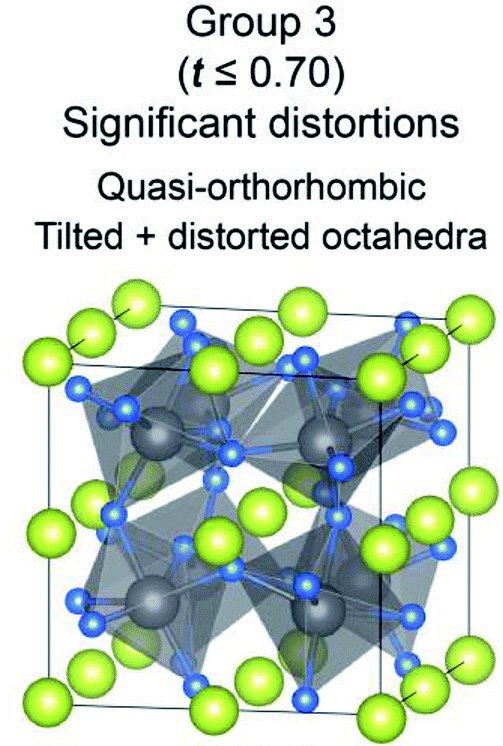
\includegraphics[height=6.5cm]{./figures/distortions_3.png}\label{fig:distortions_3}}
\caption{Variation of the anti-perovskite structure with decreasing values of tolerance factor, t.\cite{kim2019}}
\label{distortions}
\end{figure}

The Na-rich anti-perovskite \ch{Na3NO3} (ie. \ch{Na3ONO2}) was first reported in 1938 by Zintl and Morawietz,\cite{zintl1938} followed by further investigation of the structure by Klemenc and Gutmann in 1950\cite{klemenc1950} and Jansen in 1977.\cite{jansen1977}
These early works lead to a range of anti-perovskite type materials being characterised toward the end of the 20th century,\cite{fanfani1980, hippler1990b, sabrowsky1990, hippler1990c} including the archetypical alkali metal chalcogenide halides, \ch{Na3OCl} and \ch{Na3OBr} by Sabrowsky and Hippler.\cite{sabrowsky1988, hippler1990}
Soon after, conductivity studies revealed the superionic conduction properties of anti-perovskites \ch{Na3NO3} and \ch{Na3OCN} above specific temperatures due the "paddle wheel" mechanism, which is disussed later. \cite{muller1990, jansen1992}
Recently, anti-perovskites were suggested as potential solid electrolyte materials, after superionic room temperature conductivity of $>10^{-3} \ \mathrm{S \ cm^{-1}}$ was reported in Li-rich anti-perovskites in 2012.\cite{zhao2012, reckeweg2012}

Significant effort has been devoted to uncovering the mechanism for ion transport in anti-perovskites.
The two possible migration mechanisms in these materials are a simple vacancy hop and a concerted three-ion hop mechanism involving Li interstitial dumbbells.
The interstitial mechanism was found to have lower activation energy, however, it is predicted that there is six orders of magnitude greater concentration of Li vacancies than Li interstitials.
Although one study argues that oxide ions may occupy some of the vacant Cl sites, inducing the formation of interstitials,\cite{mouta2016} it is generally accepted that the vacancy migration mechanism dominates.\cite{emly2013, zhang2013, mouta2014, lu2015}

In addition to the recent work on Li-rich anti-perovskites,\cite{dawson2018a, clarke2021, shen2020} there have been conductivity studies of the sodium analogues.
In 2015, a study by Wang \textit{et al.} focused on the Na-ion conductivity of anti-perovskites with the general formula \ch{Na3OX} (X = Cl, Br or I).
A low room temperature Na-ion conductivity in the range of $10^{-8} \ \mathrm{S \ cm^{-1}}$ was measured, but it was found that this could be increased by two orders of magnitude via a combination of doping strategies.\cite{wang2015a}

There are numerous examples of isovalent doping being employed to expand the ionic lattice and increase the Na-ion conductivity of Na-rich anti-perovskites.
Some vary halogen size \cite{wang2015a, ahiavi2020, lin2020, dawson2018c, kim2019, fan2020, lu2020, yin2020}, while others replace the halides with soft hydride ions;\cite{gao2021} alternatively, the chalcogen size can also be varied.\cite{kim2019, yin2020, gao2021}
Theoretical work has also been directed at mixing Li ions on the Na sites, but this resulted in reduced conductivity.\cite{dawson2018c}
Furthermore, it was theoretically formulated that isovalent mixing the chalcogen ions in a specific manner can result in the formation of double anti-perovskites, such as \ch{Na6SOI2}, with alternating \ch{ONa6} and \ch{SNa6} octahedra.
This structure is predicted to be thermodynamically and dynamically stable with low Na-ion migration energies of 0.21 eV.\cite{yu2018}

As well as expanding the lattice, employing isovalent doping strategies may also lead to increased lattice distortions that promote ionic mobility.
Distortion in the anti-perovskite lattice can be quantised using the tolerance factor, t, described by Eq. \ref{tolerance}:
\begin{equation}
    t = \frac{r_X + r_{Na}}{\sqrt{2}(r_C + r_{Na})}
\label{tolerance}
\end{equation}
Where $r_{Na}, \ r_X \ and \ r_C$ represent the ionic radii of \ch{Na+}, the halide and the chalcide, respectively. 
While the ideal value of $t$ for anti-perovskite synthesis is $0.84 < t < 0.97$, theoretical studies showed that structures with lower values of $t$, which deviate from the ideal cubic symmetry (see Figure \ref{fig:distortions_2} and \ref{fig:distortions_3}) might enable lower energy migration pathways and lead to higher Na-ion conductivity if synthesised.\cite{kim2019, avdontceva2015, pham2018}

There are also studies on isovalent doping that make use of large cluster ions both in the monovalent anion position (superhalides such as \ch{BH4-}, \ch{NO2-}, \ch{BCl4-}, \ch{BF4-} and \ch{AlH4-})\cite{ahiavi2020, sun2019, gao2020, fang2018} and in the divalent anion position (such as \ch{SO4^{2-}}).\cite{fan2020, avdontceva2015}
It has been suggested that on top of expanding the lattice, cluster ions in might have the added benefit of aiding Na-ion transport via a rotational or "paddle wheel" mechanism, particularly at high temperatures. \cite{jansen1991}
For example, \ch{Na3OBH4} was quoted to have a Na-ion conductivity of  $4.4 \times 10^{-3} \ \mathrm{S \ cm^{-1}}$ at room temperature\cite{sun2019}, although a later study could not reproduce these results.\cite{ahiavi2020}
Overall, it has been found that isovalent doping is suitable for the fine-tuning of Na-ion conductivity in these materials.

\begin{figure}[!ht]
\centering
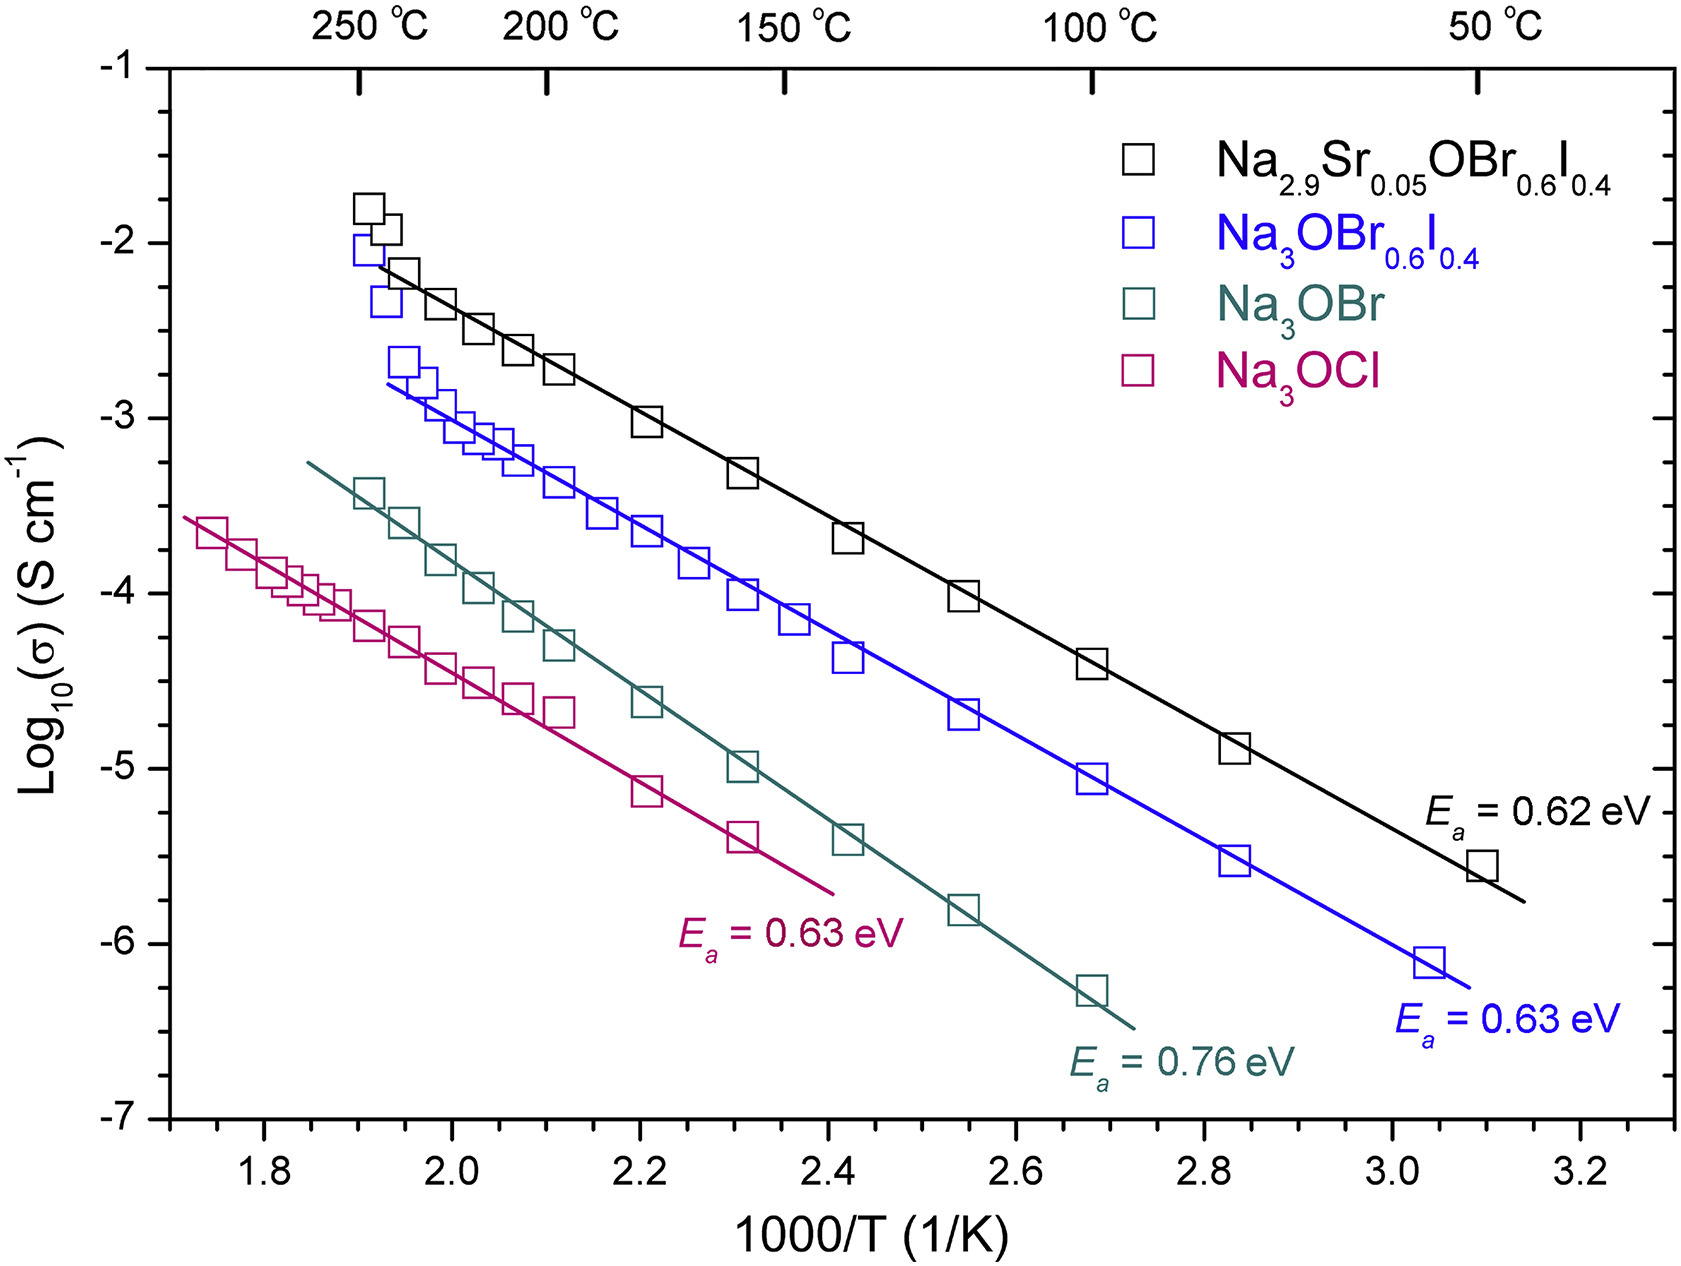
\includegraphics[width=11cm]{./figures/cond_plot.jpg}
\caption{Arrhenius plot of experimental conductivity of selected anti-perovskites at a range of temperatures. Structures with partial and complete isovalent substitution, as well as ones with a small level of aliovalent doping are included.\cite{wang2015a}}
\label{plot}
\end{figure}

Similarly to Li-rich analogues, the ion transport in Na-rich anti-perovskites was found to take place via a vacancy migration mechanism\cite{zhu2016} with alkali halide vacancies being the dominant intrinsic defect type.\cite{dawson2018c, wan2018}
Therefore, aliovalent doping to induce Na vacancies is a viable strategy to increase the Na-ion conductivity in these structures.
Divalent alkaline earth metal ions were introduced successfully to improve ionic conductivity in this manner.\cite{wang2015a, fan2020, wan2018} 
Alternatively monovalent anion doping on the chalcogen site has also been explored for vacancy generation.\cite{gao2021}
The work by Wang \textit{et al.} applied a combination of iso- and aliovalent doping strategies (see Figure \ref{plot}) and found an optimized Na-ion conductivity of $2.78 \times 10^{-6} \ \mathrm{S \ cm^{-1}}$ at room temperature for \ch{Na_{2.9}Sr_{0.05}OBr_{0.06}I_{0.04}}.\cite{wang2015a}

There is also a significant volume of promising work on low-dimensional-networked anti-perovskite-like materials.\cite{lu2020, zhu2016, yu2019}
As discussed, the cubic phase of the anti-perovskite structure involves ionic migration along the edges of the \ch{ONa6} octahedra, in a 3D manner.
Low-dimensional anti-perovskites are obtained by reducing the dimensionality of the interconnected octahedra, which was suggested to lead to an improvement in ionic conductivty.
The 2DN anti-perovskites with general formula \ch{Na4ChX2}, also known as Ruddlesden-Popper structures, present a good combination of synthesizability and predicted Na-ion conductivity up to $6.3 \times 10^{-3} \ \mathrm{S \ cm^{-1}} $ for \ch{Na3Li_{S0.5}O_{0.5}I2}.
Based on theoretical work, it is likely that structures with even lower dimensionality (1 or 0) would have low conductivities even if synthesised.\cite{lu2020}
  
\section{Project outline and aims}

Despite the recent interest in sodium-based solid electrolytes,\cite{kim2017, zhao2018} the atomic-scale factors that control the dopant properties of Na-rich anti-perovskites have not been fully characterised, which are important for the optimization of their ionic  conductivity.
In this project the overall aim is to use large-scale atomistic simulation techniques to study the defect chemistry and the effects of aliovalent doping on the Na-ion transport of \ch{Na3OCl}.
Such computational techniques have been applied successfully to a wide range of battery materials including other lithium- and sodium-ion solid electrolytes.\cite{symington2020, dawson2018b, deng2015, clarke2021, deng2018}

First, we optimize our simulation setup to ensure it can accurately reproduce structural and mechanical data from experiment.
Then, we examine the intrinsic defect chemistry by using data from isolated point defect calculations to derive defect formation energies. 
The likely mechanism of ionic migration is predicted by calculating energy profiles.
We then consider a range of divalent (Mg, Ca, Sr and Ba) and trivalent (Al and Ga) cationic dopants in terms of modes of dopant incorporation and the possibility of dopant-vacancy clustering, by performing further defect calculations as well as molecular dynamics (MD) simulations.
We collect mean square displacement data from the MD simulations to derive ionic conductivity values for the investigated structures, and also examine the Na-ion trajectories to better understand ion conduction mechanisms on the atomic scale.

In general, we aim to gain valuable insights that can guide future work towards enhancing the solid electrolyte properties of sodium-rich anti-perovskites.









\chapter{Computational Modelling Methods}

\section{Introduction}

Computational chemistry has developed into a central area of science and the theoretical characterisation of chemical systems is now a common aspect of chemistry-related research projects.\cite{jensen2017}
Simulations are used to gain valuable information on atomic-scale effects that would be difficult to probe with experimental techniques alone.
Potentials-based atomistic computational techniques offer an effective means of probing these effects over extended time periods in large-scale crystalline structures and have been applied to a wide range of battery materials.

\section{Atomistic simulations}

\subsection{Interatomic potentials}

Atomistic simulations employ interatomic potentials to describe a system as a function of the spatial coordinates of its atoms.
The set of potentials must accurately represent every possible interatomic interaction in the system, in terms of the forces acting on the atoms and the potential energy between them.
The sum of the potential energies of all the one- to n-body isolated interactions give the internal energy of the system, as shown in equation \ref{lattice}.\cite{catlow1997} 

\begin{equation}
    U = \sum_{i} U_{i}(r_{i}) + \sum_{ij} U_{ij}(r_{ij}) \ + \sum_{ijk} U_{ijk}(r_{ijk}) \ + \: ...
\label{lattice}
\end{equation}

\noindent
In an ionic lattice, the first term accounts for the interaction of ions with any external electric fields (single-body term), while the second and third account for the interactions of all ion pairs (two-body term) and ion trios (three-body term).
The expression can include interactions of larger number of ions, however, this study only considers two-body interactions as there is no external field acting on the system and higher-body terms are not expected to significantly impact the results.

The two-body term is often comprised of long- and short-range interactions that are modelled by the Coulombic and short-range terms, respectively. 

\begin{equation}
    U_{ij} = \Phi_{Coulombic}(r_{ij}) + \Phi_{short-range}(r_{ij})
\label{twobody}
\end{equation}
'
\noindent
The long-range Coulombic terms arises from pure electrostatic interactions of the pairs of charged species, and account for as much as 90\% of the total lattice energy.\cite{catlow2013}

\begin{equation}
    \Phi_{Coulombic} = \sum_{ij} \frac{q_iq_j}{4\pi\varepsilon_0r_{ij}}
\label{coulomb}
\end{equation}

\noindent
When ions are within short range of each other, their interaction is modelled using interatomic potentials derived empirically either from experimental or smaller-scale \textit{ab initio} data.
There is a variety of interatomic potentials used in the literature including Buckingham, harmonic, Lennard-Jones and Morse potentials.\cite{gale2003, buckingham1938}
Based on previous investigations on battery materials, Buckingham potentials were chosen to model short-range interactions in this work.
Buckingham potentials are described by Eq. \ref{buckingham}, where A, $\rho$ and C are parameters determined empirically.

\begin{equation}
    \Phi_{short-range} = A\exp\frac{-r_{ij}}{\rho_{ij}} - \frac{C_{ij}}{r_{ij}^6}
\label{buckingham}
\end{equation}

\noindent
The positive term represents the repulsive forces of the electronic charge cloud of ions, while the negative term models the attractive forces.
In summary, the potential energy of the two-body interactions (and hence the internal energy of the lattice) can be determined by atomistic modeling with only the knowledge of the ionic positions and charges and the three empirical parameters of the Buckingham potential.

\subsection{Polarizability}

The model outlined above considers ions as being rigid spheres, where the electrons are tightly bound to the nucleus of the ion.
Usually, this is not an accurate description of an ionic lattice, as the electron clouds tend to shift based on other ions surrounding it and this polarisation needs to be accounted for. 

The simplest way to include this effect in the simulation is the point polarizable ion (PPI) model.
This involves each ion being assigned a dipole moment ($\mu_i$) based on their point polarizability ($\alpha_i$) and the magnitude of the electric field acting upon them (E):

\begin{equation}
    \mu_i = \alpha_i E
\label{ppi}
\end{equation}

\noindent
The PPI is an inexpensive method that can produce useful results for certain structures.
However, it does not account for polarisation coupling, meaning it underestimates the polarising power of polarised ions on their neighbours.
Dick and Overhauser’s Shell Model\cite{dick1958} can describe this polarisation coupling effect better by treating each ion in the lattice as a separate core and shell.
Since the core and the shell are oppositely charged (with the sum of the charges equalling to that of the replaced point charge) they are screened by Coulombic forces, but the model links them using a harmonic spring. 
The non-polarizable core represents the nucleus of the ion and the core electrons, accounting for the entire mass of the ion.
The polarizable shell is comprised of the valence electrons, with an estimated mass of zero.
The charge of the shell, $Y$ and the spring constant of the harmonic, $k$ are derived from experimental or \textit{ab initio} data and relate to the electronic polarizability as described by equation \ref{shellm}.\cite{dick1958}

\begin{equation}
    \alpha = \frac{Y^2}{k}
    \label{shellm}
\end{equation}

\subsection{Deriving interatomic potentials}

The parameters used for atomistic simulations are derived by empirical fitting to a crystal structure along with electric and elastic data gained from experiment or \textit{ab initio} calculations.
The quality  of the fit of the parameters can be assessed using the sum of squares (SS) calculation, where the experimental ($f_i^{exp}$) and calculated ($f_i^{calc}$) values for each of the relevant observables ($N_{obs}$) are compared and scaled according to importance, using a weighing factor ($\omega_i$).

\begin{equation}
    SS = \sum_{i=1}^{N_{obs}} \omega_i (f_i^{exp} - f_i^{calc})^2
\label{sumsquares}
\end{equation}

\noindent
In a perfect model, $\mathrm{SS = 0}$, however this is very rarely the case, as the primary aim of atomistic simulations is to provide reasonable model of them system at low computational costs.
In this work, the parameters to be fitted consist of the Buckingham potential's A, $\rho$ and C terms and the Shell Model's Y and k terms.

\subsection{Energy minimisation}

Ionic systems and their internal energy are described as a function of the spatial coordinates of their ions.
Sets of ionic coordinates, $\textbf{x}$, and their associated internal energy, $U(\textbf{x})$, can be plotted on a $3N$ dimensional potential energy surface, where $N$ represents the number of ions in the system.
On the potential energy surface, there will be certain configurations, where the surface's gradient is zero with respect to all dimensions, that is $\nabla U(\textbf{x}) = 0$.
These are stationary points and there are three variants of them: maxima, minima and saddle points.

Maxima are points where $\nabla^2 U(\textbf{x}) < 0$, and appear as peaks on the potential energy surface, representing unfavourable configurations that are unlikely to exist.
On the other hand, minima, with $\nabla^2 U(\textbf{x}) > 0$ represent potential wells of favourable configurations.
Finally, there are saddle points, where $\Delta^2 U(\textbf{x}) < 0$ in some directions on the surface, while $\Delta^2 U(\textbf{x}) > 0$ in others, leading to a saddle-like structure when visualised in 3D.
On a potentials energy surface, these points represent transition states, which act as the maximum point along the most favourable energy path between two minima.

Energy minimisation techniques aim to find the lowest energy configuration of a structure.
It is important to note that there may be a number of local minima present on a potential energy surface, but only the lowest energy one represents the global minimum and the true ground state structure.\cite{bush1995}
To find this global minimum it is essential that minimisation techniques are provided with good initial conditions derived from experiment or \textit{ab initio} calculations.
The simplest energy minimisation techniques involve scanning the parameter space to find the global minimum. 
However, these methods are inefficient and computationally expensive and instead gradient-based methods are often employed.
The internal energy of a system at a point $(\textbf{x} + \delta\textbf{x})$ can be expressed as a Taylor series expression based on point $\textbf{x}$:

\begin{equation}
    U(\textbf{x} + \delta\textbf{x}) = U(\textbf{x}) + \frac{\partial U}{\partial \textbf{x}} \delta \textbf{x} + \frac{1}{2} \frac{\partial^2 U}{\partial \textbf{x}^2} (\delta \textbf{x})^2 + ... + \frac{1}{n} \frac{\partial^n U}{\partial \textbf{x}^n} (\delta \textbf{x})^n
\label{taylor}
\end{equation}

\noindent
This expression can be truncated after the second term, leaving the internal energy at a given point, $U(\textbf{x})$ and a first derivative vector, $\textbf{g}$, which describes the direction from point \textbf{x} that results in the steepest increase in $U(\textbf{x})$.

\subsubsection{Steepest descent}

The simplest gradient-based method is the steepest descent algorithm, where the atomic coordinates are changed in a way that likely leads to the largest decrease in energy.
The position \textbf{x} is moved by a distance $\delta$, whose magnitude can be determined either arbitrarily or via a line search.
The next position is given by:

\begin{equation}
    \textbf{x}_{p+1} = \textbf{x}_p - \textbf{g}_p \delta
\end{equation}
 
 \noindent
The method eventually converges on a minimum through a series of orthogonal successive steps. 
While this method is convenient for finding minima far from the initial starting point, it is not considered efficient for finding the exact configuration, as this would require a large number of small steps.

\subsubsection{Conjugate gradient}

An improvement is the conjugate gradient method, which uses a set of search vectors and minimises the energy along each one of them.
Initially, the the energy is minimised along the vector $-\textbf{g}_p$.
Then, once the minimum is found, the new search vector ($\textbf{b}_p$) is given by:

\begin{equation}
    \textbf{d}_p = -\textbf{g}_p + \beta_{p} \textbf{d}_{p-1}
\end{equation}
Where:
\begin{equation}
    \beta = \frac{\textbf{g}_p.\textbf{g}_p}{\textbf{g}_{p-1}.\textbf{g}_{p-1}}
\end{equation}

\noindent
Energy is minimised along the search vector, followed by the evaluation of a new search vector and the process is repeated until the calculations converge.
Using this method has the advantage of being quicker than the steepest descent approach, if the starting point is near the minimum.
It can converge in as few as $3N$ steps for a $N$ body system if the potential energy surface in the search region is quadratic.

\subsubsection{Newton-Raphson}

For the steepest descent and conjugate gradient method, the Taylor expansion describing the potential energy surface (Eq. \ref{taylor}) is truncated after the second term, hence they are labelled as first order methods.
The Newton-Raphson minimisation is a more complex second order method, where the third term of the Taylor expression is also included, yielding a Hessian matrix, $\textbf{H}$.
Then, the $\textbf{x}_{p+1}$ position on the potential energy surface is found using a combination of the first and second derivatives:

\begin{equation}
    \textbf{x}_{p+1} = \textbf{x}_p - \textbf{g}_p \textbf{H}_p^{-1}
\end{equation}

\noindent
The Newton-Raphson method has the ability of finding the minimum energy configuration in a single step, if the potential energy surface is quadratic in the search region.
However, this is rarely the case, so the method must be applied iteratively.
Furthermore, the minimisation is highly expensive and can even become unstable if the starting point is far from the minimum.
Therefore, if there is no reliable experimental data available, a combination of the steepest descent or conjugate gradient and the Newton-Raphson method is often applied to reduce computational expense.

\section{Periodic boundary conditions}

Real crystal systems contain too  a very high number of atoms making them impossible to model in their entirety. 
Idealising the system as infinite allows the utilisation of periodic boundary conditions, so that only a small region of the crystal needs to be considered.
The smallest possible pattern that represents the crystal is known as a unit cell.
Depending on the aim of the work, the "main" simulation area can be chosen to be a single unit cell or a collection of unit cell known as a supercell.
Regardless, periodic boundary conditions copy the "main" simulation area and attach these copies to the boundaries of the chosen region.

Now, the "main" simulation is part of a larger lattice and the ions inside it can interact with each other and with the ions residing in the copies.
However, the ions in the copies may only interact with the ions inside the "main" simulation and not with each other.
Furthermore, in dynamic systems, when an ion leaves the main simulation, it is reintroduced at the opposite side of the system with the same dynamic properties as before.
In summary, the ions of the "main" simulation are self-contained and the copies are only there to make these ions experience the forces that would act upon them in a large lattice.

\section{Defect modelling}

Defect chemistry is a vital part of understanding and improving the atomic-scale ionic conductivity of solids (See Appendix A).
When a defect is introduced to a system, the structure of the lattice will slightly change around it and the system can no longer be modelled as an array of symmetrical unit cells.
The Mott-Littleton approximation takes this into account and attempts to model the defect at an infinite dilution, by splitting the lattice into two regions.  

The sphere nearest the defect (Region I) include the defect and the ions surrounding it. 
This region of the lattice is relaxed explicitly to account for the great degree of disorder and employs both Buckingham potentials and Coulombic forces for the minimisation. 
The outer region (Region II) then covers the rest of the lattice and is further divided into sub-regions IIa and IIb. 
In Region IIa, the ions experience a harmonic interaction with the defect and thus in this region the interaction of the central charge defect and the ions is modelled with Coulombic forces exclusively. 
The ions in Region IIb are sufficiently far from the defect that its effects are only felt in a dielectric manner.
Hence, this region is modelled using a dielectric continuum, where there is no actual displacement of ions, only a change in polarisation.\cite{mott1938}

\section{Molecular dynamics}

The techniques outlined thus far model systems at absolute zero temperatures.
However, as ionic motion is a kinetic effect, modelling at temperatures above 0 K is essential.
Molecular dynamics (MD) techniques allow the investigation of the movement of ions in dynamic systems over time, based on Newton's Second Law of Motion linking the force acting on a species (\textbf{F}) to its acceleration (\textbf{a}).\cite{frenkel2001}

\begin{equation}
    \textbf{F} = m\textbf{a}
    \label{newton}
\end{equation}

\subsection{Integration Algorithms}

As discussed before, the forces acting on an ion depend on its position relative to all other ions in the lattice.
Of course, in a dynamic system, the ionic positions change over time, so to explore ionic motion, these forces must be evaluated repeatedly over infinitesimally small time intervals, $\Delta t$.
It is important to chose an appropriate value for this time step.
The value must be smaller than any atomic-scale process that could affect the investigated properties, such as atomic vibrations, in the order of nanoseconds.
Using small time steps helps avoid instabilities in the system from ions accelerating to unphysical velocities then colliding.
On the other hand, small time steps lead to increased computational costs, so typically the chosen values is between 0.1-1 femtoseconds.

The exact position, $\textbf{r}$, of an ion $i$ at $t + \Delta t$ is given by the Taylor expansion:

\begin{equation}
    \textbf{r}_i(t + \Delta t) = \textbf{r}_i(t) + \textbf{r}^{\prime}_i(t) \Delta t + \frac{1}{2} \textbf{r}^{\prime\prime}_i(t) \Delta t^2 + \frac{1}{6} \textbf{r}^{\prime\prime\prime}_i(t) \Delta t^3 + ...
    \label{taylor_2}
\end{equation}

\noindent
This can also be expressed as:

\begin{equation}
    \textbf{r}_i(t + \Delta t) = \textbf{r}_i(t) + \textbf{v}_i(t) \Delta t + \frac{1}{2} \textbf{a}_i(t) \Delta t^2 + \frac{1}{6} \textbf{b}_i(t) \Delta t^3 + ...
\end{equation}

\noindent
Where $\textbf{v}_i(t)$, $\textbf{a}_i(t)$ and $\textbf{b}_i(t)$ represent the velocity, acceleration and jerk of ion $i$ at time $t$.
Then, using Eq. \ref{newton} and some rearranging, the most useful form is found:

\begin{equation}
    \textbf{r}_i(t + \Delta t) = \textbf{r}_i(t) + \Delta t \ \textbf{v}_i(t) + \frac{\Delta t^2}{2m_i} \textbf{f}_i(t) + \frac{\Delta t^3}{6} \textbf{b}_i(t) + ...
\end{equation}

\noindent
Where $\textbf{f}_i(t)$ is the overall force acting on ion $i$ at time $t$.
The velocity of the ion can also be described similarly, resulting in:

\begin{equation}
    \textbf{v}_i(t + \Delta t) = \textbf{v}_i(t) + \frac{\Delta t}{m_i} \textbf{f}_i(t) + \frac{\Delta t^2}{2} \textbf{b}_i(t) + ...
\end{equation}

\noindent
These differential equation are difficult to solve for a many-body system, but integration algorithms find ways to approximate them efficiently.

\subsubsection{Euler algorithm}

The Euler integration algorithm truncates Eq. \ref{taylor_2} after the second derivative.
This effectively means that over the period $\Delta t$ the forces acting on an ion are assumed to be constant and so acceleration is uniform.
In this case, after the time step $t + \Delta t$, the position ($\textbf{r}$) and velocity ($\textbf{v}$) of ion $i$ can be evaluated based on their previous values and the acceleration ($\textbf{a}$) calculated.

\begin{equation}
    \textbf{r}_i(t + \Delta t) = \textbf{r}_i(t) + \Delta t \ \textbf{v}_i(t) + \frac{\Delta t^2}{2m_i} \textbf{f}_i(t) + \Theta (\Delta t^3)
\end{equation}

\begin{equation}
    \textbf{v}_i(t + \Delta t) = \textbf{v}_i(t) + \frac{\Delta t}{m_i} \textbf{f}_i(t) + \Theta (\Delta t^2)
\end{equation}

\noindent
The last term, $\Theta$ represents the error originating from the truncation of the Taylor expression. In this case the error on the ionic position is of third order, while that for the velocity is of second order.
This relatively large error for the velocity is significant, as in a MD simulation, the velocity of the particles in used to find their kinetic energies and the overall temperature of the system.
Therefore, the large error could lead to unwanted fluctuations in the temperature of the simulation.
This effect can be reduced by using small values of $\Delta t$, but this increases computational costs.

\subsubsection{Verlet algorithm}

The Verlet algorithm is a more sophisticated integration method, which also takes into account the jerk of the ion, $\textbf{b}_i$.

\begin{equation}
    \textbf{r}_i(t+\Delta t) = \textbf{r}_i(t) + \Delta t \ \textbf{v}_i(t) + \frac{\Delta t^2}{2m_i} \textbf{f}_i(t) + \frac{\Delta t^3}{6} \textbf{b}_i(t) + \Theta (\Delta t^4)
    \label{next}
\end{equation}

\noindent
While $\textbf{b}_i$ is difficult to compute, it can be implicitly included by considering some information about the system from the previous step, $\textbf{r}_i(t-\Delta t$).

\begin{equation}
    \textbf{r}_i(t+\Delta t) = \textbf{r}_i(t) - \Delta t \ \textbf{v}_i(t) + \frac{\Delta t^2}{2m_i} \textbf{f}_i(t) - \frac{\Delta t^3}{6} \textbf{b}_i(t) + \Theta (\Delta t^4)
    \label{last}
\end{equation}

\noindent
Summing Eqs. \ref{next} and \ref{last} and rearranging leads to a model that accounts for the jerk term without the need for it to be calculated.

\begin{equation}
    \textbf{r}_i(t+\Delta t) = 2\textbf{r}_i(t) + \frac{\Delta t^2}{m_i}\textbf{f}_i(t) - \textbf{r}_i(t+\Delta t) + \Theta (\Delta t^4)
\end{equation}

\noindent
It is important to note that the summation process also means that the calculation of the velocity is skipped.
This is significant because the way velocity is calculated yields a larger error term, once again requiring small values of $\Delta t$, as shown in Eq. \ref{verlet_error}. 

\begin{equation}
    \textbf{v}_i(t) = \frac{\textbf{r}_i(t+ \Delta t) - \textbf{r}_i(t-\Delta t)}{2 \Delta t} + \Theta(\Delta t^2)
    \label{verlet_error}
\end{equation}

\noindent
A variation of the Verlet algorithm, known as the velocity-Verlet algorithm, can help reduce this error in the velocity term to $\Theta(\Delta t^3)$, by considering $\textbf{f}_i(t+\Delta t$).

\subsection{Equilibration}

MD simulations typically begin by an energy minimisation, followed by the initialisation process.
The integration algorithms outlined are not self-starting, meaning the initial velocities of the ions must be assigned for the simulation to begin.
These are assigned in a random manner to produce a system with the desired temperature, and no net momentum.

\begin{equation}
    \sum_{i=1}^N m_i \textbf{v}_i^2 = 3Nk_bT
    \label{boltzmann}
\end{equation}

\begin{equation}
    \sum_{i=1}^N m_i \textbf{v}_i = 0
\end{equation}

\noindent
After the initial assignment of velocities, the system is allowed to run until it reaches an equilibrium, which ensures that no single ion has unphysical velocities.
The kinetic energy of the ions and the internal energy of the system is monitored during this period and the equilibrium is said to be reached when these properties reach a steady state.

\subsection{Ensembles}

An ensemble describes a set of thermal states that a system might access during the simulation.
These accessible states are specified by applying certain constraints on the system.

\subsubsection{Micro-canonical ensemble}

The constrains in an ensemble are applied by setting certain properties of the system to a constant value.
In case of the micro-canonical ensemble, these properties are the number of ions ($N$), the volume of the simulation cell ($V$) and the total energy of the system ($E$).
While useful in some cases, the micro-canonical ensemble permits large fluctuations in the temperature and pressure of the system, which is not realistic for the ionic structures investigated here.

\subsubsection{Canonical ensemble}

In the canonical ensemble, the number of ions ($N$), the volume ($V$) and the temperature ($T$) of the system are set to be constant.
Whilst it is relatively straightforward to constrain N and V, T is calculated using ionic velocities (Eq. \ref{boltzmann}), which gives raise to rounding errors and potentially some variation.
To keep temperature constant, a thermostat is commonly used, which couples the system to a heat sink, which is set to the target temperature.

\subsubsection{Isobaric-isothermal ensemble}

The isobaric-isothermal ensemble keeps the number of ions ($N$), the pressure ($P$) and the temperature ($T$) constant in the simulation cell.
Again, $T$ varies over time, but in addition, $P$ also needs adjusting.
Similarly to the way $T$ is controlled, $P$ is kept constant using a barostat.

\subsection{Analysing MD data}

MD simulations can provide a host of useful output data, based on the positions and velocities of ions in the simulation after each time step.

\subsubsection{Conductivtity}

The mean square displacement (MSD) describes the average value an ion has moved from its initial position over a given period of time.

\begin{equation}
    \mathrm{MSD}(t) = \frac{1}{N} \sum_{i=1}^N \Big\{ \textbf{r}_i (t) - \textbf{r}_i(t_0) \Big\}^2
\end{equation}

\noindent
Plotting the MSD for the charge carrier species (ususally Li or Na) against time and taking the slope allows the calculation of the diffusion coefficient.

\begin{equation}
    D = \frac{\partial\mathrm{MSD}(t)}{\partial t}
\end{equation}

\noindent
From this, the ionic conductivity of the material and the activation barrier for energy migration can be determined.

\begin{equation}
    \sigma = \frac{q^2n\mu}{k_B T}
\end{equation}

\begin{equation}
    ln(\sigma T) = -\frac{E_a}{k_BT} 
\end{equation}

\subsubsection{Ionic trajectories}

The data gained from MD simulations can be visualised by tracing and connecting the positions of ions over the duration of the simulation.
The level of detail these plots reveal depends on the intervals between the recorded positions.
Noting position every few steps is useful for giving detail about the ionic migration paths, while leaving more time between recorded frames allows for dopant and grain boundary effects to be explored.

\clearpage










\chapter[Results and Discussion]{Results and Discussion:
\textnormal{Atomic-scale investigation of cation doping and defect clustering in the anti-perovskite \ch{Na3OCl} sodium-ion conductor}}

\section{Introduction}

Solid-state lithium- and sodium-ion batteries are attracting growing interest due to their enhanced safety and higher energy density compared to conventional liquid electrolyte cells, as outlined in Chapter 1.\cite{famprikis2019, zhang2018b, ohno2020, bachman2016, manthiram2017, gao2018, kim2017, zhao2018, dawson2018b}
A wide range of Li- and Na-based structures have been investigated for potential use as solid electrolytes.  
One such family of ionic conductors that has been attracting significant attention is characterized by the anti-perovskite structure.  
Anti-perovskite materials possess a number of promising properties for solid electrolyte applications, such as high ionic conductivity, negligible electronic conductivity, wide electrochemical windows\cite{dawson2021, wang2020b} and favourable mechanical behaviour,\cite{khandy2020, sattar2021, lv2017, deng2016, wang2016b, ramanna2013, zinenko2012} which allow them to be integrated into solid-state batteries. 
Another important aspect of the perovskite structure is that it is highly amenable to chemical substitution or ion doping in order to fine-tune mechanical or transport properties for a given application. 

In addition to recent work on Li-rich anti-perovskites \ch{Li3OX} (X = Cl or Br),\cite{zhao2012, emly2013, dawson2018a, clarke2021, shen2020} there have been structural and conductivity studies of the sodium analogues \ch{Na3OX} (X = Cl or Br)\cite{sabrowsky1988, hippler1990, wang2015a, zhu2016, nguyen2016, wan2018, dawson2018c, pham2018, kim2019, ahiavi2020, lin2020, li2021}, as well as work on a range of other Na-rich anti-perovskites such as \ch{Na3OBH4}.\cite{jansen1977, fanfani1980, muller1990, jansen1992, avdontceva2015, fang2018, sun2019, gao2020, fan2020, yin2020, gao2021, sabrowsky1990, hippler1990b, yu2018, yu2019, lu2020}
In comparison to lithium, Na-ion batteries have the advantages of raw material abundance and reduced cost with possible use in large-scale grid storage applications. 
It is generally accepted that ion transport in Na-rich anti-perovskites takes place via Na vacancy migration\cite{zhu2016} as sodium vacancies seem to be the majority sodium defect species.  Therefore, one approach of potentially increasing Na-ion conductivity is doping with aliovalent cations at the sodium sites to increase the concentration of mobile sodium vacancies.\cite{wang2015a, wan2018}  

Despite the recent interest in sodium-based solid electrolytes,\cite{kim2017, zhao2018} the atomic-scale factors that control the dopant properties of Na-rich anti-perovskites have not been fully characterized, which are important for the optimization of their ionic conductivity. 
In this study, we use large-scale atomistic simulations to study a range of divalent (Mg, Ca, Sr and Ba) and trivalent (Al and Ga) cation dopants and their impact on the Na-ion transport properties of \ch{Na3OCl}. 
We examine the modes of dopant incorporation and the possibility of dopant-vacancy association or clustering to gain new insights into the fundamental factors that could influence macroscopic sodium-ion conduction. 

\section{Methodology}

Atomistic simulation methods have been applied to a wide range of solid-state compounds including Li- and Na-ion battery materials.\cite{clarke2021, islam2014, deng2018, tapia2018, symington2020}
However, there are only a few examples\cite{dawson2018c, li2021} of these methods being applied to Na-rich anti-perovskites.
The use of such atomistic simulations can provide valuable insight into ion diffusion over longer timescales and greater lattice sizes than ab initio methods.  

As discussed in Chapter 2, short- and long-range interactions are modelled with Buckingham-type interatomic potentials and Coulombic forces, respectively.\cite{catlow1997} 
The shell model of Dick and Overhauser\cite{dick1958} is implemented to account for ionic polarization. 
The parameters used in this work are listed in the Table \ref{potentials}. 
The new Na-O, Na-Cl and Ga-Cl potentials were derived empirically using the experimental structures of \ch{Na3OCl} and \ch{GaCl3}. 
For the defect energy calculations, the two-region Mott-Littleton approach\cite{mott1938} is utilised, as included in the General Utility Lattice Program (GULP).\cite{gale2003} 
Molecular dynamics (MD) calculations are performed using the LAMMPS code\cite{plimpton1995} and are run for 10 ns with 1 fs timesteps on a large supercell containing $\mathrm{\sim}$17,000 atoms. 
Sodium vacancies are distributed randomly in the structure, while the corresponding positively charged defects (Cl vacancy or dopant) are arranged in a regular pattern such that the spacing between these species is maximised. 
The temperature range for the simulations is 600-900 K with 100 K intervals in an NPT ensemble using a Nosé-Hoover thermostat.\cite{evans1985}
Mean square displacement (MSD) data derived from the simulations are used to obtain the diffusion coefficient. 
Conductivities are then calculated from these diffusion coefficient via the Nernst-Einstein equation for solid-state diffusion\cite{mehrer2007} with a Haven ratio of 1, as in previous studies.\cite{clarke2021, dawson2018c}
Activation energies are derived using the slopes of the linear fitting of Arrhenius conductivity plots.  

\section{Structural modelling}

During the early stages of the project, it was found that some of the Buckingham potentials (Na-O and Na-Cl) taken from the literature did not produce consistent results for certain defect calculations.
Therefore, a new, more reliable set of interatomic potentials were developed using experimental structural and mechanical data as parameters.

The calculation of the Na vacancy defect energy with a range of different radius values (10-20 \AA) for the explicitly modelled region (region \RomanNumeralCaps{1}) produced a very small variation in the defect energy of only 0.04 eV, compared to 3.41 eV with the literature values.
Therefore, it was established that the fitted potentials produced significatly more consistent results for defect calculations and these potentials were used for the rest of the work.
The full list of potentials and calculated lattice energies are presented in Tables \ref{potentials} and \ref{lattice_energy}, respectively.

\begin{table}[H]
\centering
\sidesubfloat[]{
\begin{tabular}{ l c c c }
 \hline
 \textbf{Ion Pair} & \textbf{A (eV)} & \textbf{$\rho$ (\AA)} & \textbf{C (eV \AA$^{-6}$)} \\ 
 \hline\xrowht[()]{5pt}
 \ch{Na+} - \ch{Na+} \ \cite{binks1994} & 1788.19 & 0.1590 & 0.0 \\
 \xrowht[()]{5pt}
 \ch{Na+} - \ch{O^{2-}} [This work] & 588.38 & 0.3880 & 0.0 \\
 \xrowht[()]{5pt}
 \ch{Na+} - \ch{Cl-} [This work] & 1170.41 & 0.3150 & 0.0 \\
 \xrowht[()]{5pt}
 \ch{O^{2-}} - \ch{O^{2-}} \ \cite{mouta2014} & 22764.30 & 0.1490 & 13.19 \\
 \xrowht[()]{5pt}
 \ch{O^{2-}} - \ch{Cl-} \ \cite{binks1994} & 8286.91 & 0.2590 & 62.20 \\
 \xrowht[()]{5pt}
 \ch{Cl-} - \ch{Cl-} \ \cite{catlow1977} & 1227.20 & 0.3210 & 14.53 \\
 \hline\xrowht[()]{5pt}
 \ch{Mg^{2+}} - \ch{O^{2-}} \ \cite{darco1997} & 1428.50 & 0.2945 & 0.0 \\
 \xrowht[()]{5pt}
 \ch{Mg^{2+}} - \ch{Cl-} \ \cite{islam1990} & 4914.54 & 0.2570 & 0.0 \\
 \xrowht[()]{5pt}
 \ch{Ca^{2+}} - \ch{O^{2-}} \ \cite{darco1997} & 1090.40 & 0.3437 & 0.0 \\
 \xrowht[()]{5pt}
 \ch{Ca^{2+}} - \ch{Cl-} \ \cite{islam1990} & 2302.00 & 0.3402 & 0.0 \\
 \xrowht[()]{5pt}
 \ch{Sr^{2+}} - \ch{O^{2-}} \ \cite{darco1997} & 959.10 & 0.3721 & 0.0 \\
 \xrowht[()]{5pt}
 \ch{Sr^{2+}} - \ch{Cl-} \ \cite{clarke2021} & 2191.09 & 0.3457 & 0.0 \\
 \xrowht[()]{5pt}
 \ch{Ba^{2+}} - \ch{O^{2-}} \ \cite{darco1997} & 905.07 & 0.3976 & 0.0 \\
 \xrowht[()]{5pt}
 \ch{Ba^{2+}} - \ch{Cl-} \ \cite{clarke2021} & 2704.55 & 0.3528 & 0.0 \\
 \xrowht[()]{5pt}
 \ch{Al^{3+}} - \ch{O^{2-}} \ \cite{desouza2003} & 1725.00 & 0.2897 & 0.0 \\
 \xrowht[()]{5pt}
 \ch{Al^{3+}} - \ch{Cl-} \ \cite{clarke2021} & 1736.12 & 0.2917 & 0.0 \\
 \xrowht[()]{5pt}
 \ch{Ga^{3+}} - \ch{O^{2-}} \ \cite{khan1998} & 2901.12 & 0.2742 & 0.0 \\
 \xrowht[()]{5pt}
 \ch{Ga^{3+}} - \ch{Cl-} [This work] & 924.20 & 0.3428 & 0.0 \\
 \hline
\end{tabular}}
\label{buck}

\vspace{0.5cm}

\sidesubfloat[]{
\begin{tabular}{ l c c }
 \hline
 \textbf{Species} & \textbf{Shell charge (e)} & \textbf{Spring constant (eV \AA$^{-2}$)} \\ 
 \hline\xrowht[()]{5pt}
 \ch{Na+} & Rigid-ion & - \\
 \xrowht[()]{5pt}
 \ch{O^{2-}} \ \cite{mouta2014} & -2.183 & 593.716 \\
 \xrowht[()]{5pt}
 \ch{Cl-} \ \cite{catlow1977} & -2.485 & 29.380 \\
 \hline\xrowht[()]{5pt}
 \ch{Mg^{2+}} \ \cite{darco1997} & 1.585 & 361.6 \\
 \xrowht[()]{5pt}
 \ch{Ca^{2+}} \ \cite{darco1997} & 3.135 & 110.2 \\
 \xrowht[()]{5pt}
 \ch{Sr^{2+}} \ \cite{darco1997} & 3.251 & 71.7 \\
 \xrowht[()]{5pt}
 \ch{Ba^{2+}} \ \cite{darco1997} & 9.203 & 495.2 \\
 \xrowht[()]{5pt}
 \ch{Al^{3+}} & Rigid-ion & - \\
 \xrowht[()]{5pt}
 \ch{Ga^{3+}} & Rigid-ion & - \\
 \hline
\end{tabular}}
\label{shell}

\caption{Parameters used in this work: (a) interatomic Buckingham potentials; (b) shell model.}
\label{potentials}
\end{table}

\begin{table}[H]
\centering

\begin{tabular}{ l c }
 \hline
 \textbf{Compound} & \textbf{Lattice energy (eV)} \\ 
 \hline\xrowht[()]{5pt}
 \ch{Na3OCl} & -34.68 \\
 \xrowht[()]{5pt}
 NaCl & -8.01 \\
 \xrowht[()]{5pt}
 \ch{Na2O} & -26.38 \\
 \hline\xrowht[()]{5pt}
 \ch{MgCl2} & -26.52 \\
 \xrowht[()]{5pt}
 \ch{CaCl2} & -21.15 \\
 \xrowht[()]{5pt}
 \ch{SrCl2} & -21.14 \\
 \xrowht[()]{5pt}
 \ch{BaCl2} & -20.16 \\
 \xrowht[()]{5pt}
 \ch{AlCl3} & -55.85 \\
 \xrowht[()]{5pt}
 \ch{GaCl3} & 51.61 \\
 \hline
\end{tabular}
\caption{Lattices energies calculated for this work based on the parameters from Table \ref{potentials}}
\label{lattice_energy}
\end{table}

\section{Defect chemistry and dopant incorporation}

The starting point of the modelling study was to reproduce the experimentally observed crystal structure using potentials-based techniques (see Methods section for details), which have been applied successfully to a rich variety of battery electrode and solid electrolyte materials.\cite{clarke2021, dawson2018c, islam2014} 
The anti-perovskite crystal structure of \ch{Na3OCl} shown in Figure 1 consists of oxide ions at the typical B-site of an \ch{ABX3} perovskite, coordinated to six \ch{Na+} ions at the X-site, and the large \ch{Cl-} ion occupying the 12-coordinate A-site. 
The calculated lattice parameter for the structure is 4.406 Å, which compares well with the experimental value of 4.496 Å; the same is found for the Na-O and Na-Cl bond lengths with the mean deviations less than 0.05 and 0.06 Å, respectively.\cite{hippler1990}

\begin{figure}[h]
\centering
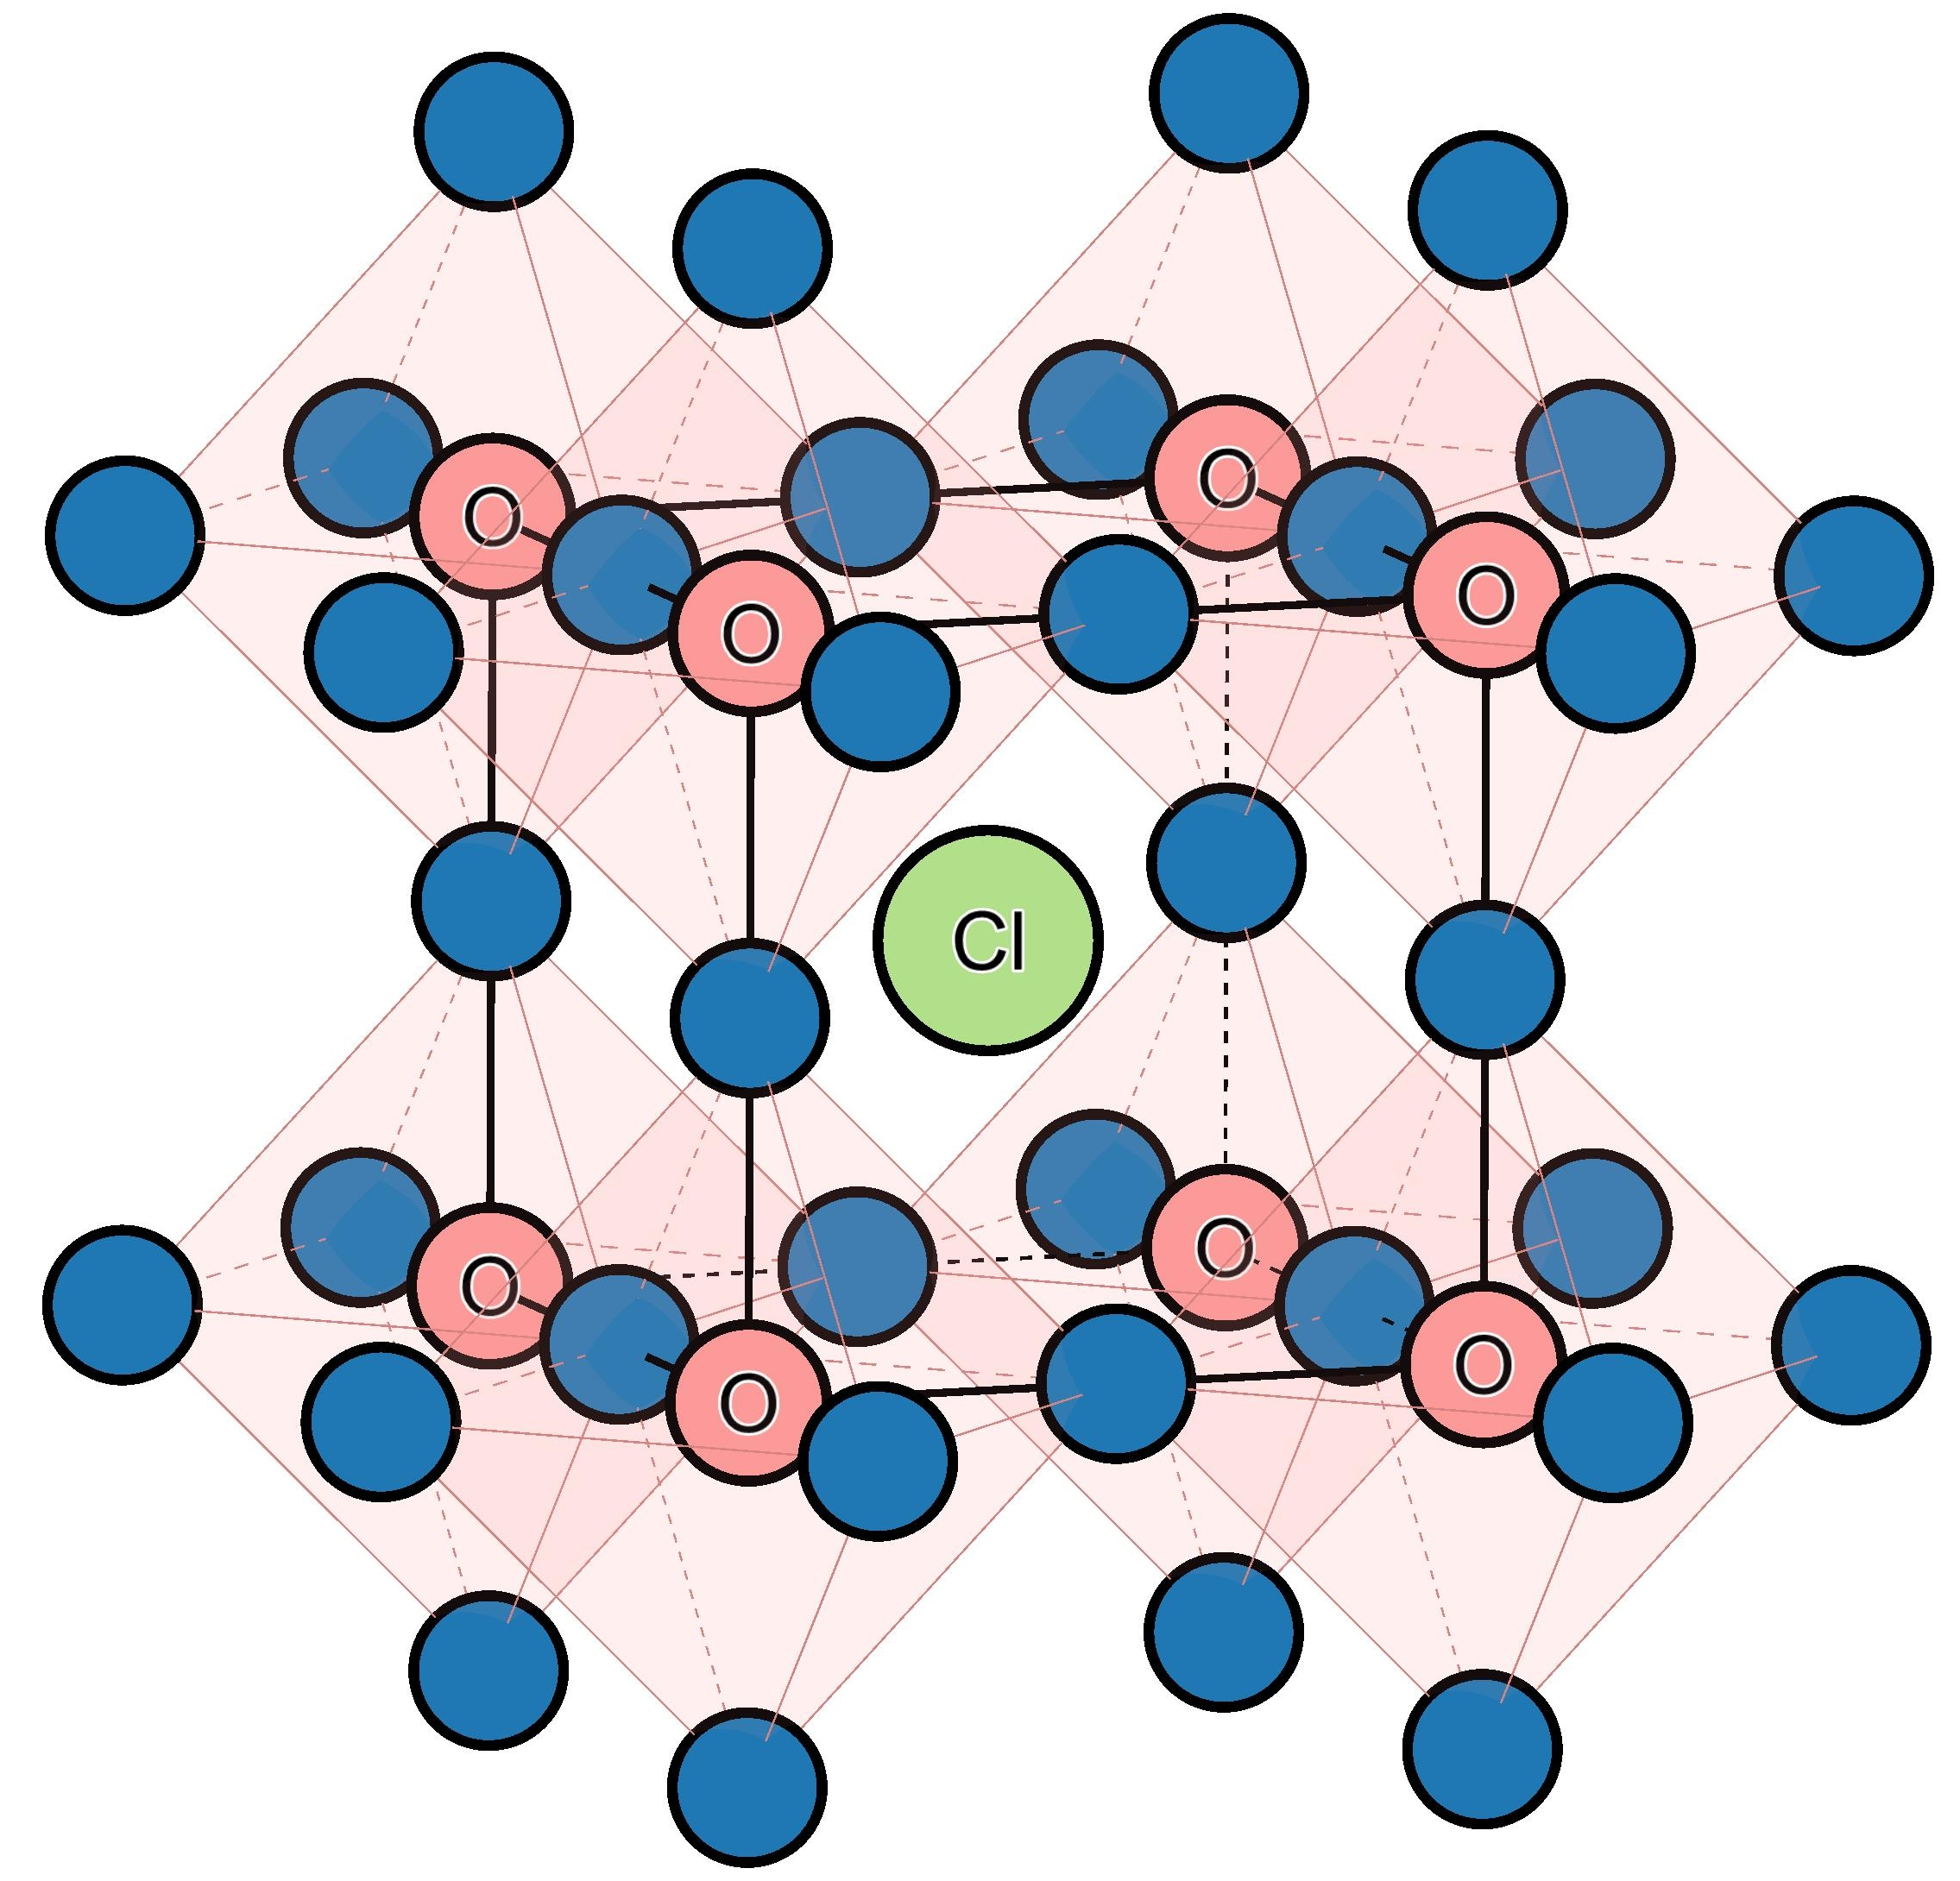
\includegraphics[width=10cm]{./figures/structure_inverted_nolabel.jpeg}
\caption{The \ch{Na3OCl} anti-perovskite structure highlighting the corner-sharing \ch{ONa6} octahedra available for Na-ion migration. Na ions are shown in blue.}
\label{structure}
\end{figure}

To probe the intrinsic defect chemistry of \ch{Na3OCl}, a series of isolated point defect (vacancy and interstitial) energies were calculated. 
By combining these energies, the relative energies of formation of Frenkel and Schottky-type defects were determined. 
The general equations (using Kröger–Vink notation) and their formation energies are presented in Table \ref{def_e} revealing two main points. 
First, the most favourable type of intrinsic defect for \ch{Na3OCl} is found to be the NaCl Schottky-type comprised of Na and Cl vacancies, in agreement with previous work;\cite{wan2018, dawson2018c} the magnitude of the formation energy suggests a very low concentration at ambient temperatures. 
Second, the formation of oxide-ion vacancies and interstitials are highly unfavourable, and unlikely to occur in any significant concentration in the undoped material; these results confirm the structural stability of the perovskite framework.

\begin{table}[h]
\centering

\resizebox{\textwidth}{!}{%
\begin{tabular}{ l l c c }
\hline
 \textbf{Defect} & \textbf{Defect reaction} & & \textbf{E (eV)} \\ 
 \hline\xrowht[()]{10pt}
 \ch{Na3OCl} Schottky & $\mathrm{3 \ Na_{Na}^{\times} + O_{O}^{\times} + Cl_{Cl}^{\times} \rightarrow 3 V_{Na}^{\prime} + V_{O}^{\bullet\bullet} + V_{Cl}^{\bullet} + \ch{Na3OCl}} $ & (3.1) & 6.74 \\
 \hline\xrowht[()]{10pt}
 \ch{NaCl} Schottky & $\mathrm{Na_{Na}^{\times} + Cl_{Cl}^{\times} \rightarrow V_{Na}^{\prime} + V_{Cl}^{\bullet} + \ch{NaCl}}$ & (3.2) & 1.96 \\
 \hline\xrowht[()]{10pt}
 \ch{Na2O} Schottky & $\mathrm{2 \ Na_{Na}^{\times} + O_{O}^{\times} \rightarrow 2 V_{Na}^{\prime} + V_{O}^{\bullet\bullet} + \ch{Na2O}}$ & (3.3) & 5.06 \\
 \hline\xrowht[()]{10pt}
 Na Frenkel & $\mathrm{Na_{Na}^{\times} \rightarrow V_{Na}^{\prime} + Na_{i}^{\bullet}}$ & (3.4) & 2.58 \\
 \hline\xrowht[()]{10pt}
 O Frenkel & $\mathrm{O_{O}^{\times} \rightarrow V_{O}^{\bullet\bullet} + O_i^{\prime\prime}}$ & (3.5) & 7.64 \\
 \hline\xrowht[()]{10pt}
 Cl Frenkel & $\mathrm{Cl_{Cl}^{\times} \rightarrow V_{Cl}^{\bullet} + Cl_{i}^{\prime}}$ & (3.6) & 3.68 \\
 \hline
\end{tabular}}
\caption{Formation energies for possible intrinsic defects in \ch{Na3OCl}.}
\label{def_e}
\end{table}

\addtocounter{equation}{6}

Our simulation methods can probe dopant incorporation in \ch{Na3OCl} by generating relative energies of dopant substitution, providing a valuable systematic guide to trends in dopant solubility.  

In this study, we have examined a wider range of aliovalent cationic dopants in \ch{Na3OCl} than experimental reports, by considering doping with divalent (Mg, Ca, Sr and Ba) and trivalent cations (Al and Ga). 
The type of charge-compensating mechanism for such dopants is often assumed to be Na vacancies, but this has not been clearly established and could also involve compensation by Cl interstitials; the two doping mechanisms for \ch{M^{2+}} and \ch{M^{3+}} cations at the Na site are described by the reactions described by Eqs. (\ref{dop1})-(\ref{dop4}).

\begin{equation}
\mathrm{2 \ Na_{Na}^{\times} + \ch{MCl2} \rightarrow M_{Na}^{\bullet} + V_{Na}^{\prime} + 2 \ NaCl}
\label{dop1}
\end{equation}

\begin{equation}
\mathrm{Na_{Na}^{\times} + \ch{MCl2} \rightarrow M_{Na}^{\bullet} + Cl_{i}^{\prime} + NaCl}
\label{dop2}
\end{equation}

\begin{equation}
\mathrm{3 \ Na_{Na}^{\times} + \ch{MCl3} \rightarrow M_{Na}^{\bullet\bullet} + 2 \ V_{Na}^{\prime} + 3 \ NaCl}
\label{dop3}
\end{equation}

\begin{equation}
\mathrm{Na_{Na}^{\times} + \ch{MCl3} \rightarrow M_{Na}^{\bullet\bullet} + 2 \ Cl_{i}^{\prime} + NaCl}
\label{dop4}
\end{equation}

\noindent
where $\mathrm{M_{Na}^{\bullet} \ and \ M_{Na}^{\bullet\bullet}}$ signify \ch{M^{2+}} and \ch{M^{3+}} dopant substitutional defects, respectively. We therefore calculated the overall substitution energy for the two different compensation mechanisms (with the dopant potentials and lattice energies listed in Table \ref{lattice_energy}).  

The resulting dopant incorporation (or ‘solution’) energies are presented in Figure \ref{doping}, which indicate two main features. 
First, Mg, Ca, Al and Ga dopants on the Na site with Na vacancy compensation are the most energetically favourable mode of dopant incorporation; these results confirm the creation of Na vacancies that are crucial for Na-ion conductivity. 
In general, the unfavourable dopants (Sr and Ba) were more than 1.5 eV higher in energy.  
Second, doping with \ch{Cl-} interstitial compensation is relatively unfavourable suggesting that such a compensation mechanism is highly unlikely in the anti-perovskite structure; indeed, such interstitial defects have not been observed experimentally. 

\begin{figure}[H]
\centering
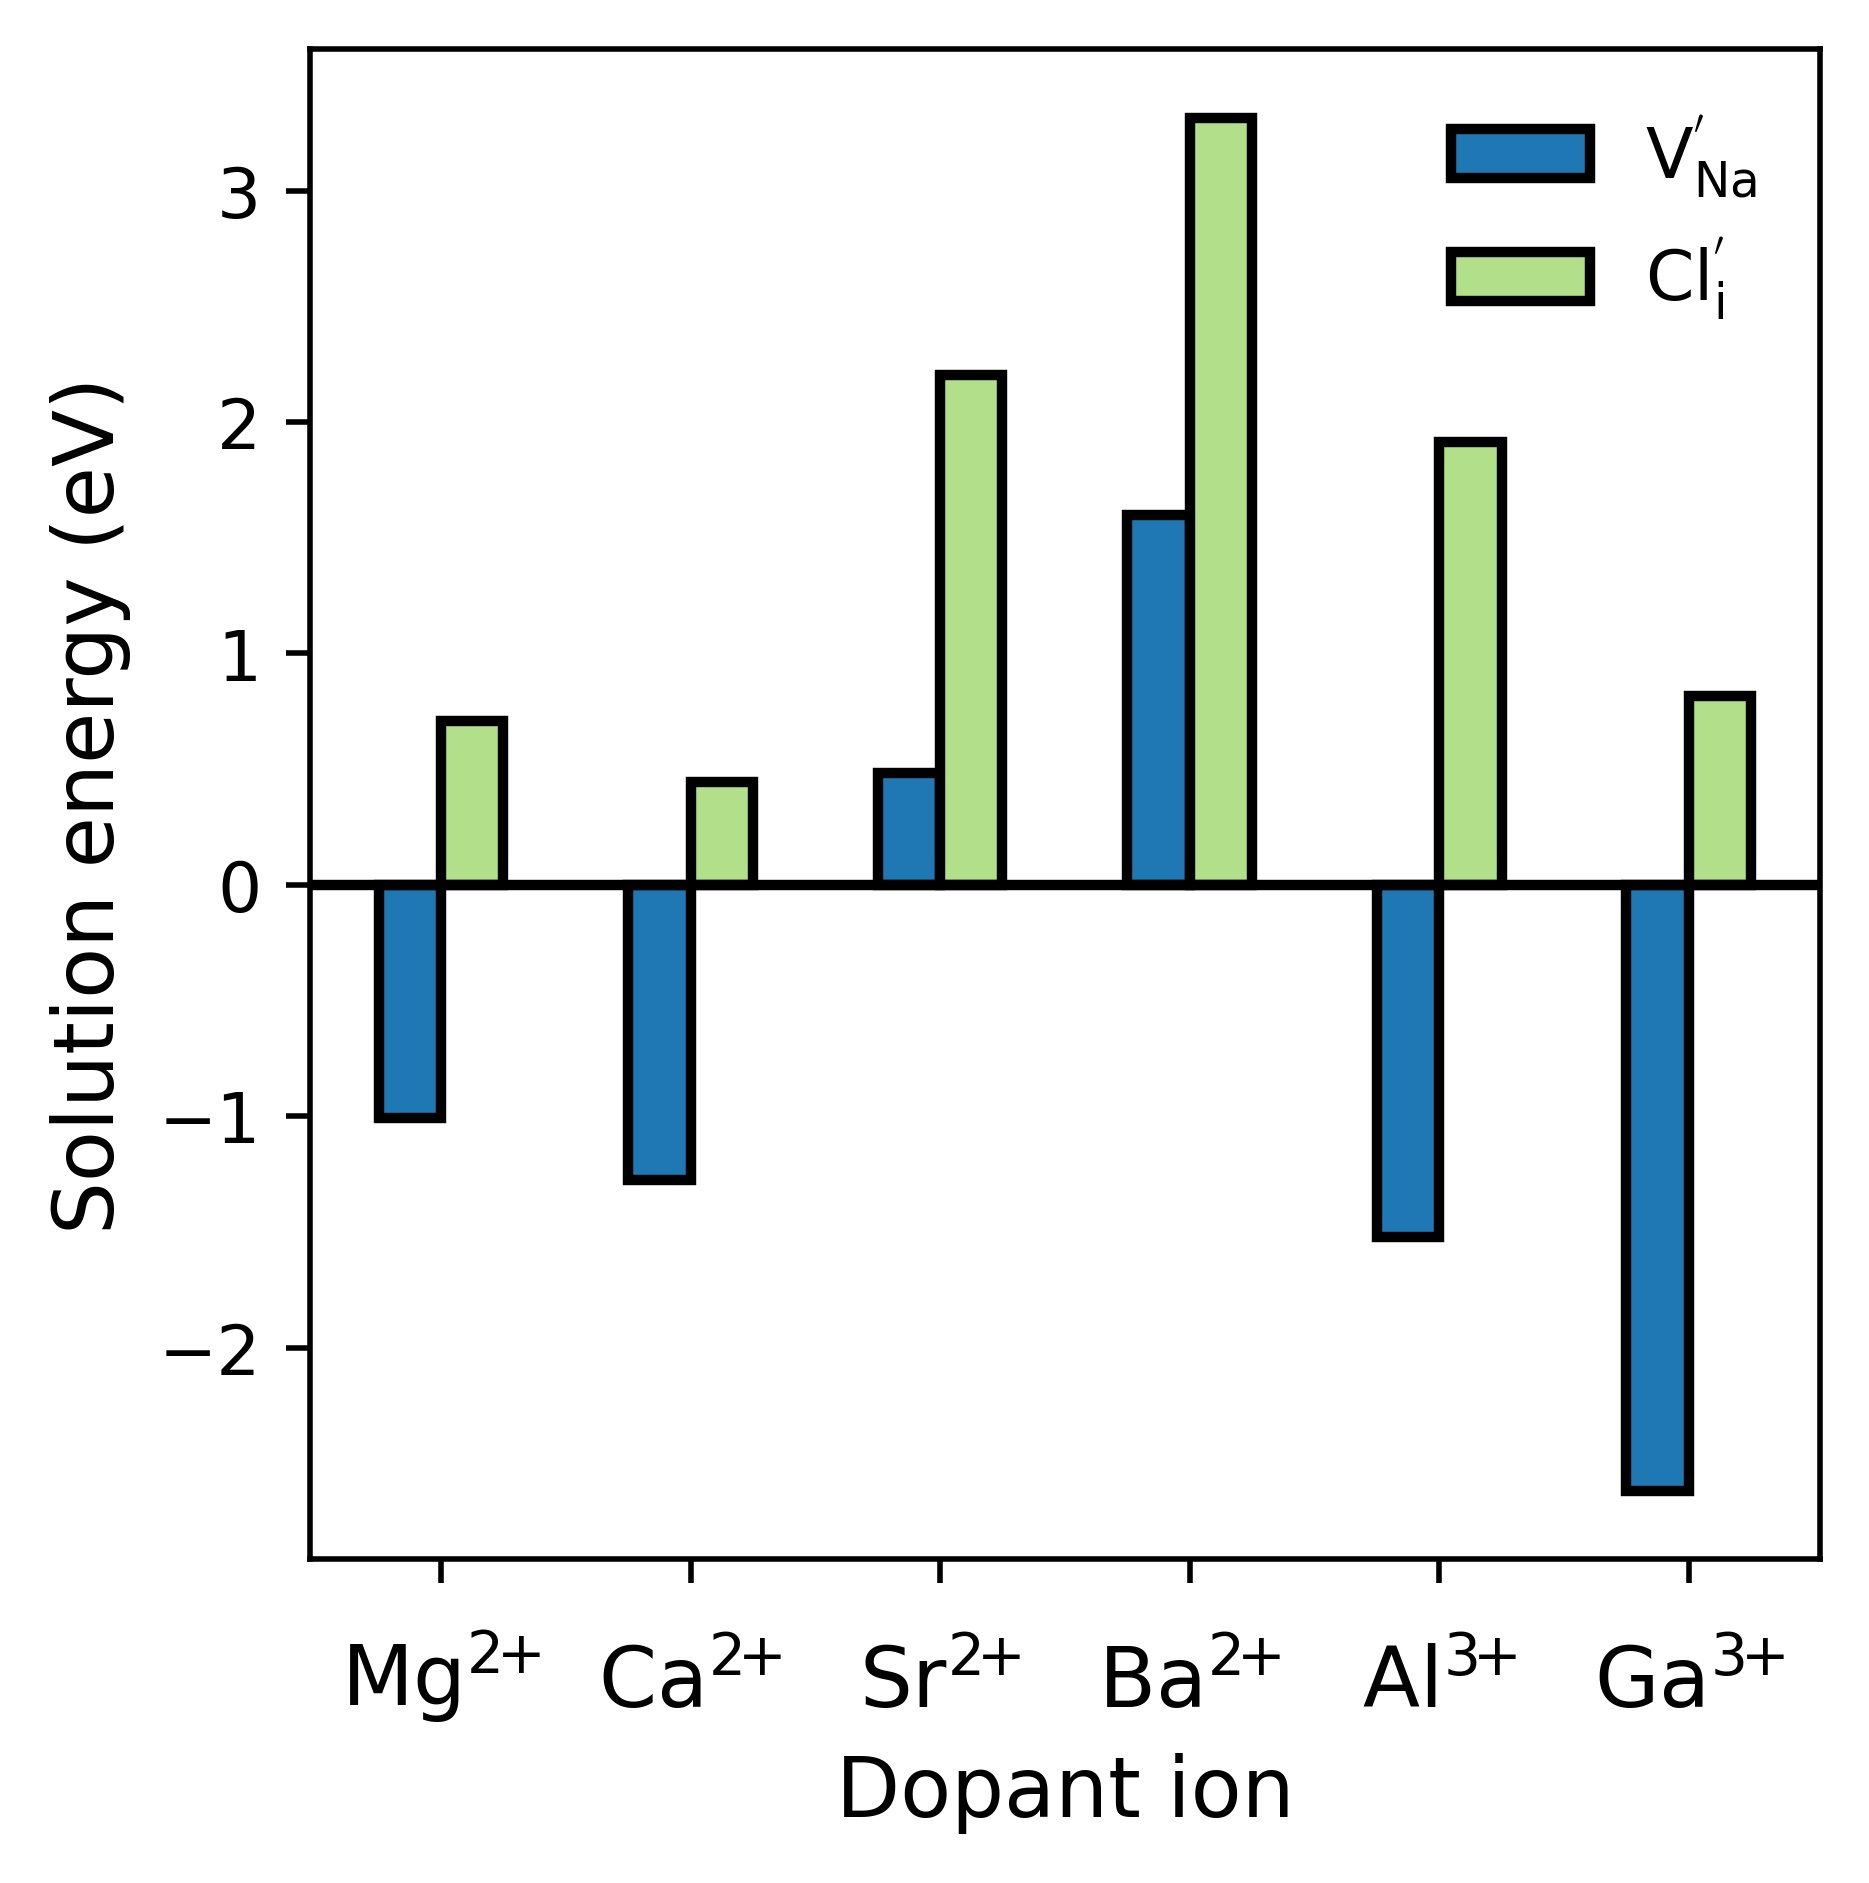
\includegraphics[width=9cm]{./figures/doping.jpg}
\caption{Dopant solution energies for \ch{M^{2+}} and \ch{M^{3+}} doping in \ch{Na3OCl} based on Eqs. (\ref{dop1})-(\ref{dop4}). Metal chlorides were used as doping agents in the reactions.}
\label{doping}
\end{figure}

\section{Na-ion conductivity and dopant-vacancy association}

Insights into Na-ion mobility and clustering effects at the atomic level are of importance when considering key solid electrolyte properties. 
However, obtaining such details for complex mixed-anion structures is far from straightforward. 
Here, molecular dynamics (MD) simulation techniques are used to investigate the Na-ion conduction properties for Mg-, Ca-, Al- and Ga-doped materials, as the most energetically favourable dopants. 
We note that our analysis using large supercells ($>17,000$ ions) and long timescales (10 ns), which are orders of magnitude greater than those currently attainable by DFT methods. 
The dopant concentrations were chosen in the range of previous experimental studies on the aliovalent doping on sodium-based anti-perovskites.\cite{wang2015a, fan2020} For the undoped system, a low level of Na vacancies (via NaCl Schottky defects) is introduced to facilitate Na conduction.

\begin{figure}
    \subfloat[Undoped, 0.1\%]{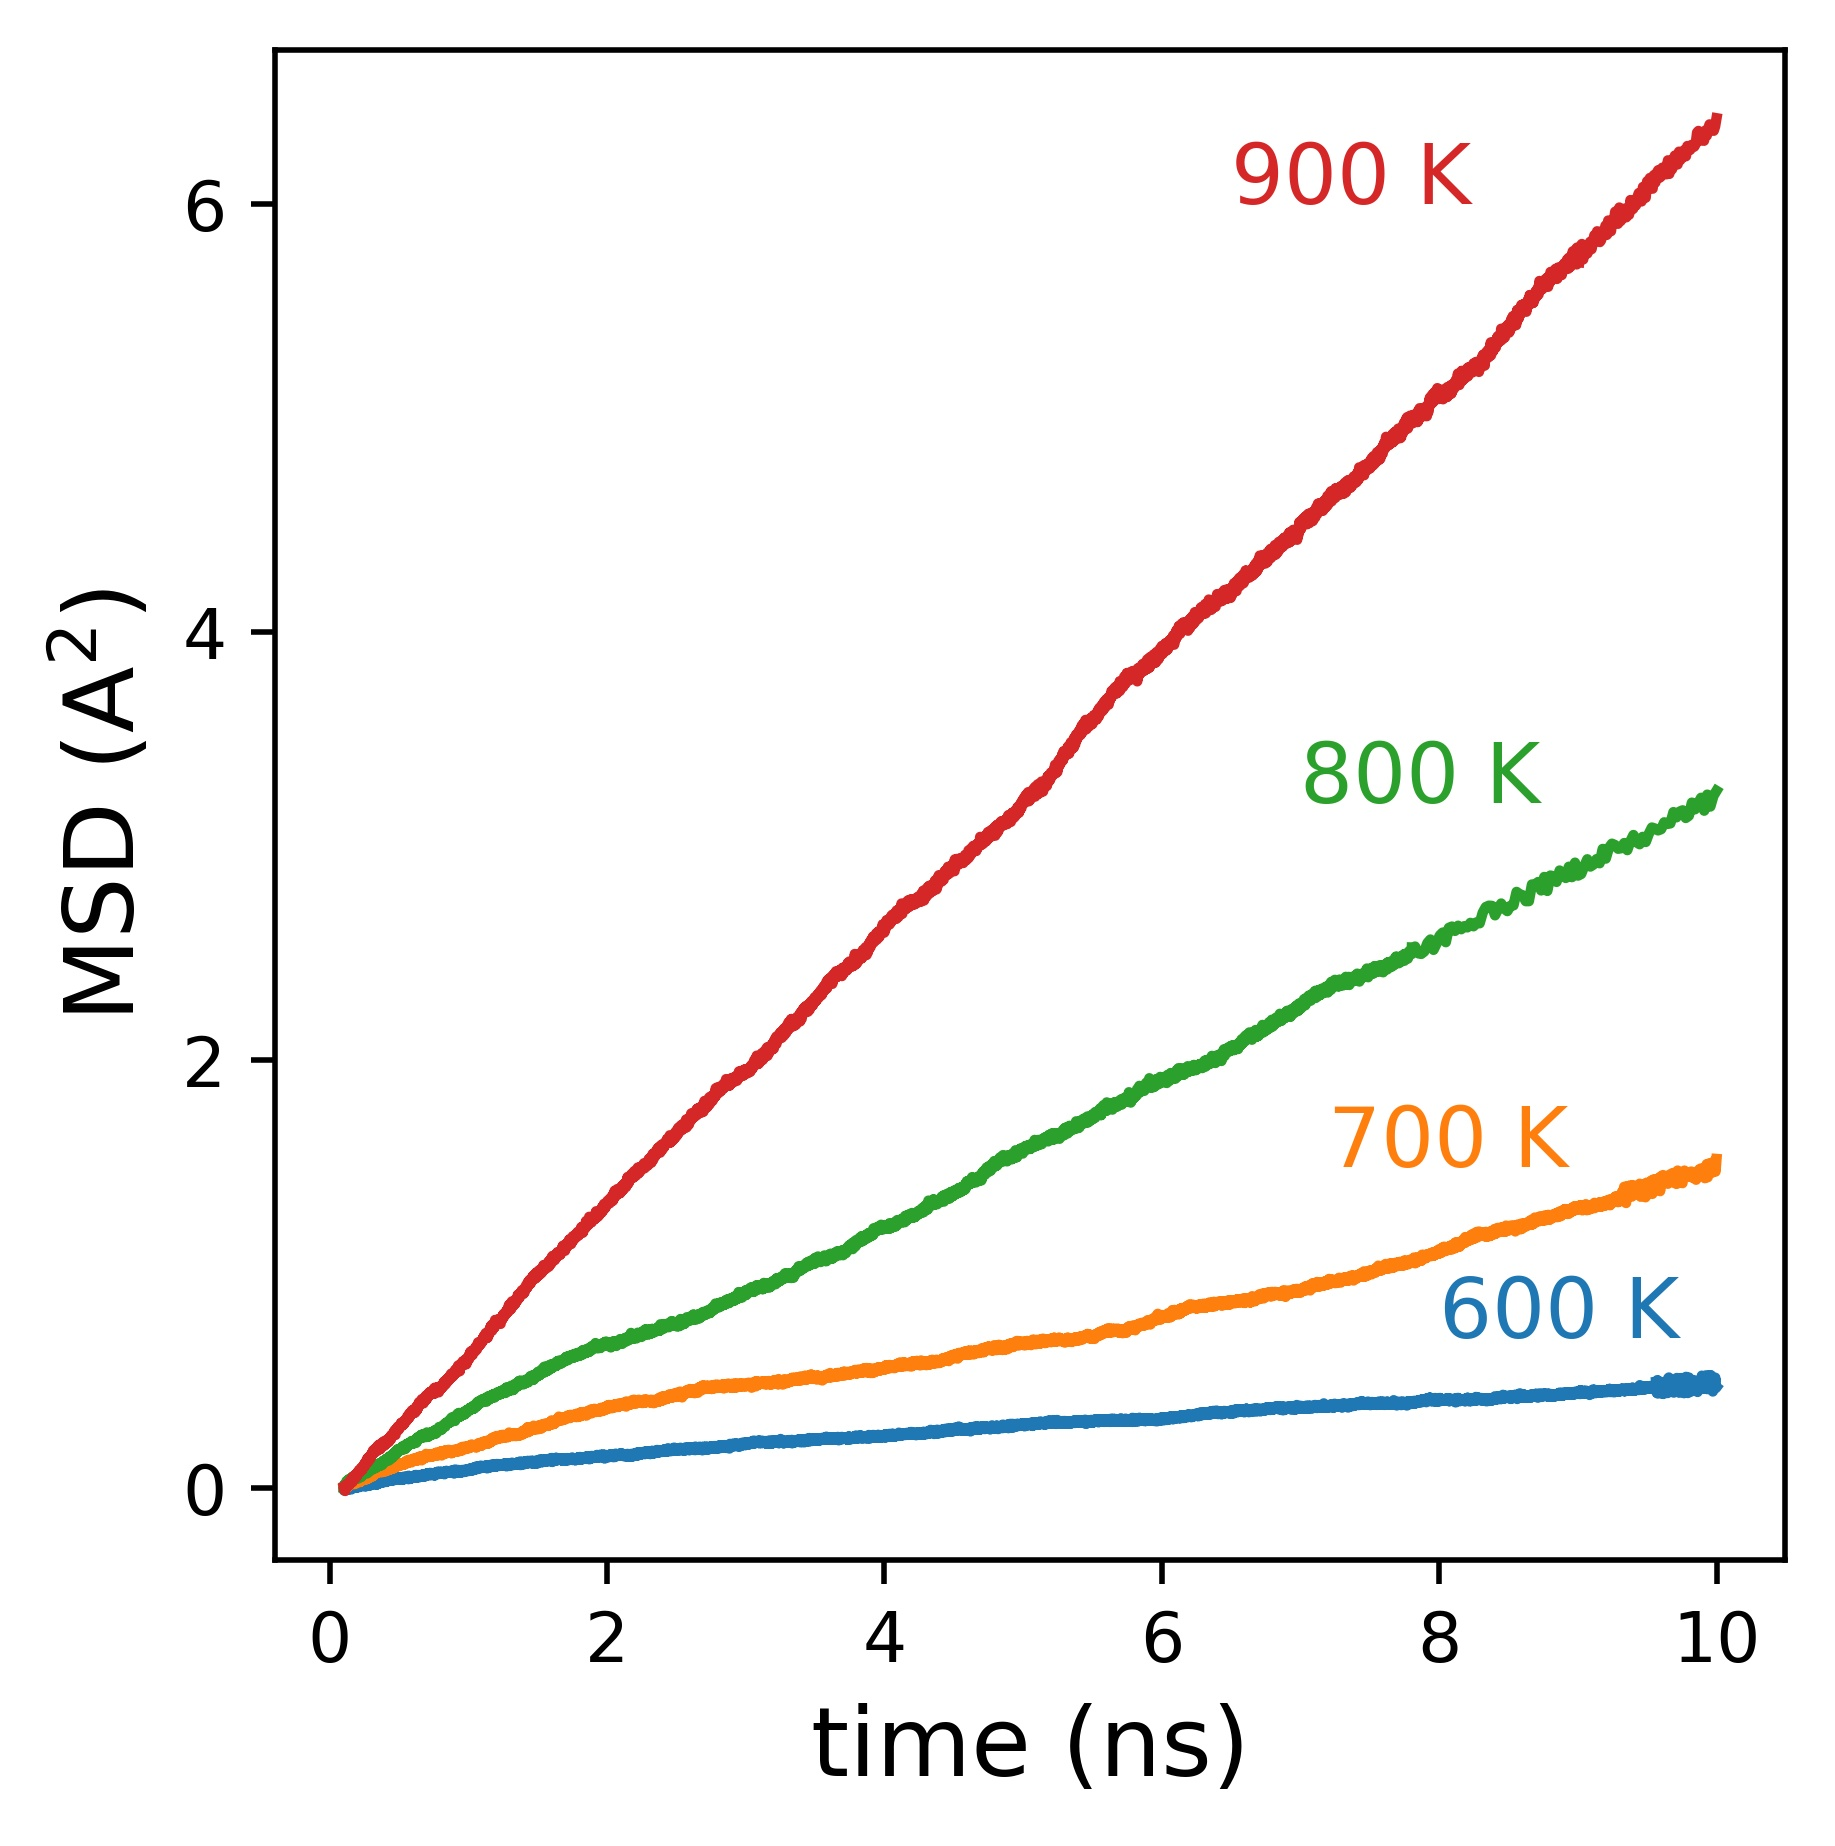
\includegraphics[height=5.4cm]{./figures/ud_msd.jpg}}
    \hspace{0.4cm}
    \subfloat[Mg-doped, 1.2\%]{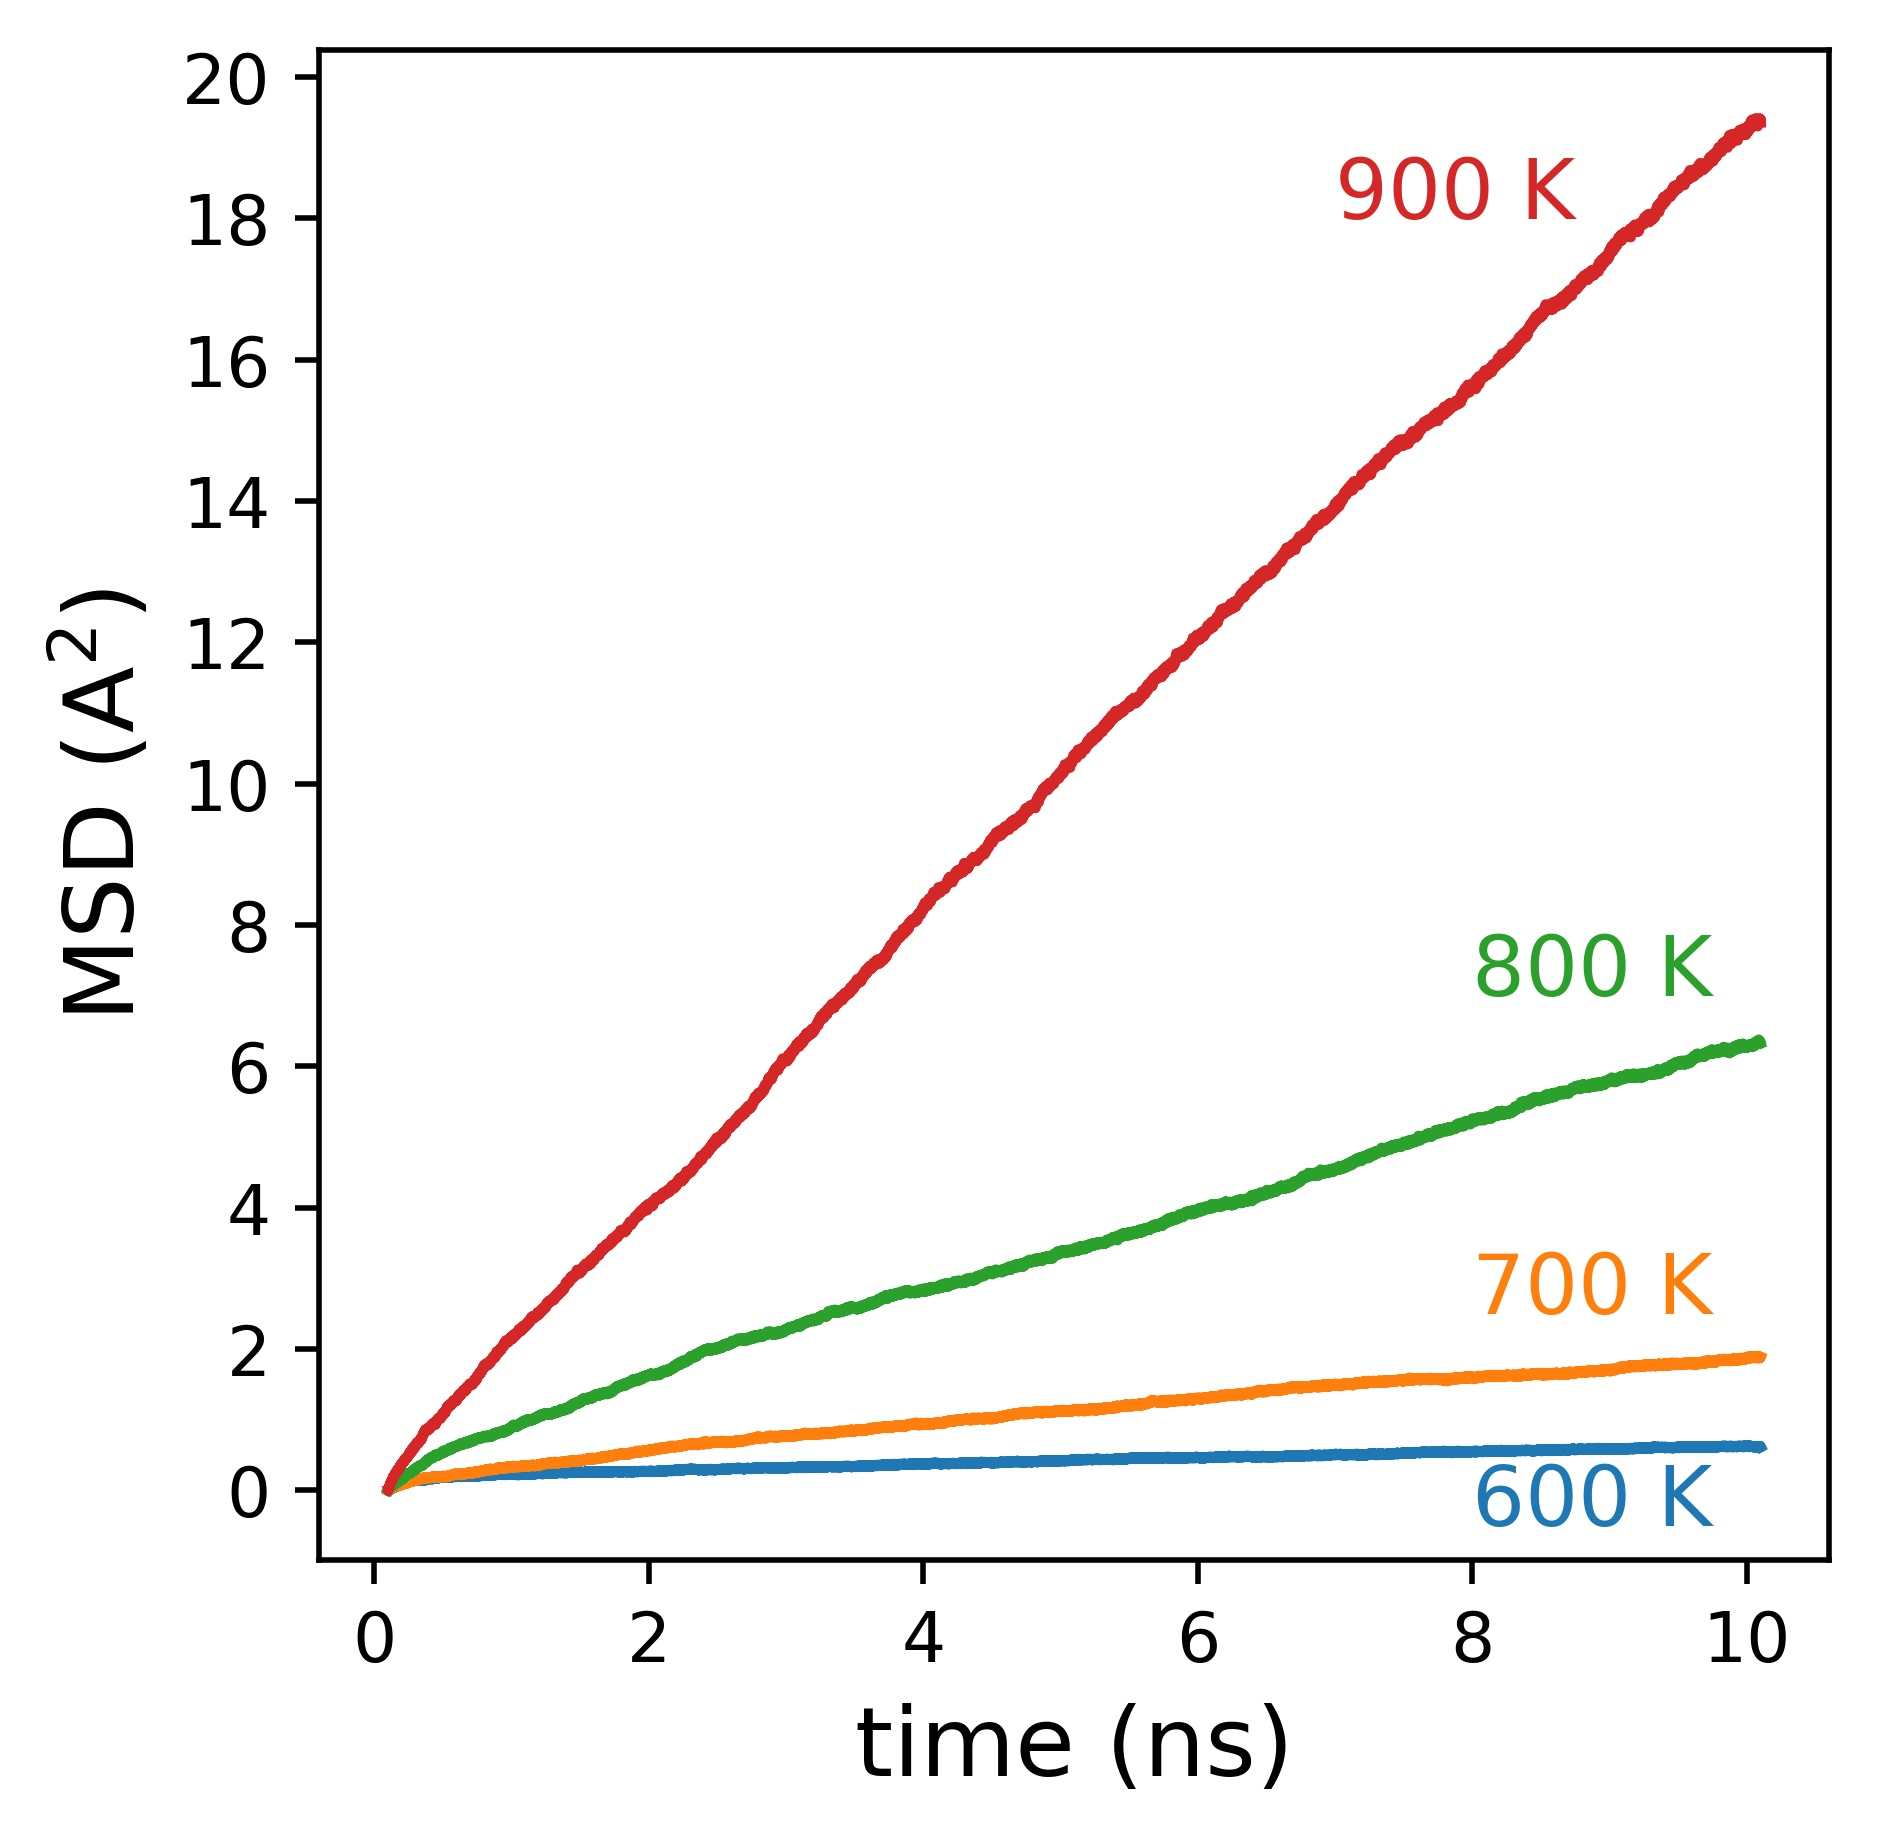
\includegraphics[height=5.4cm]{./figures/mg_msd.jpg}}
    
    \subfloat[Ca-doped, 1.2\%]{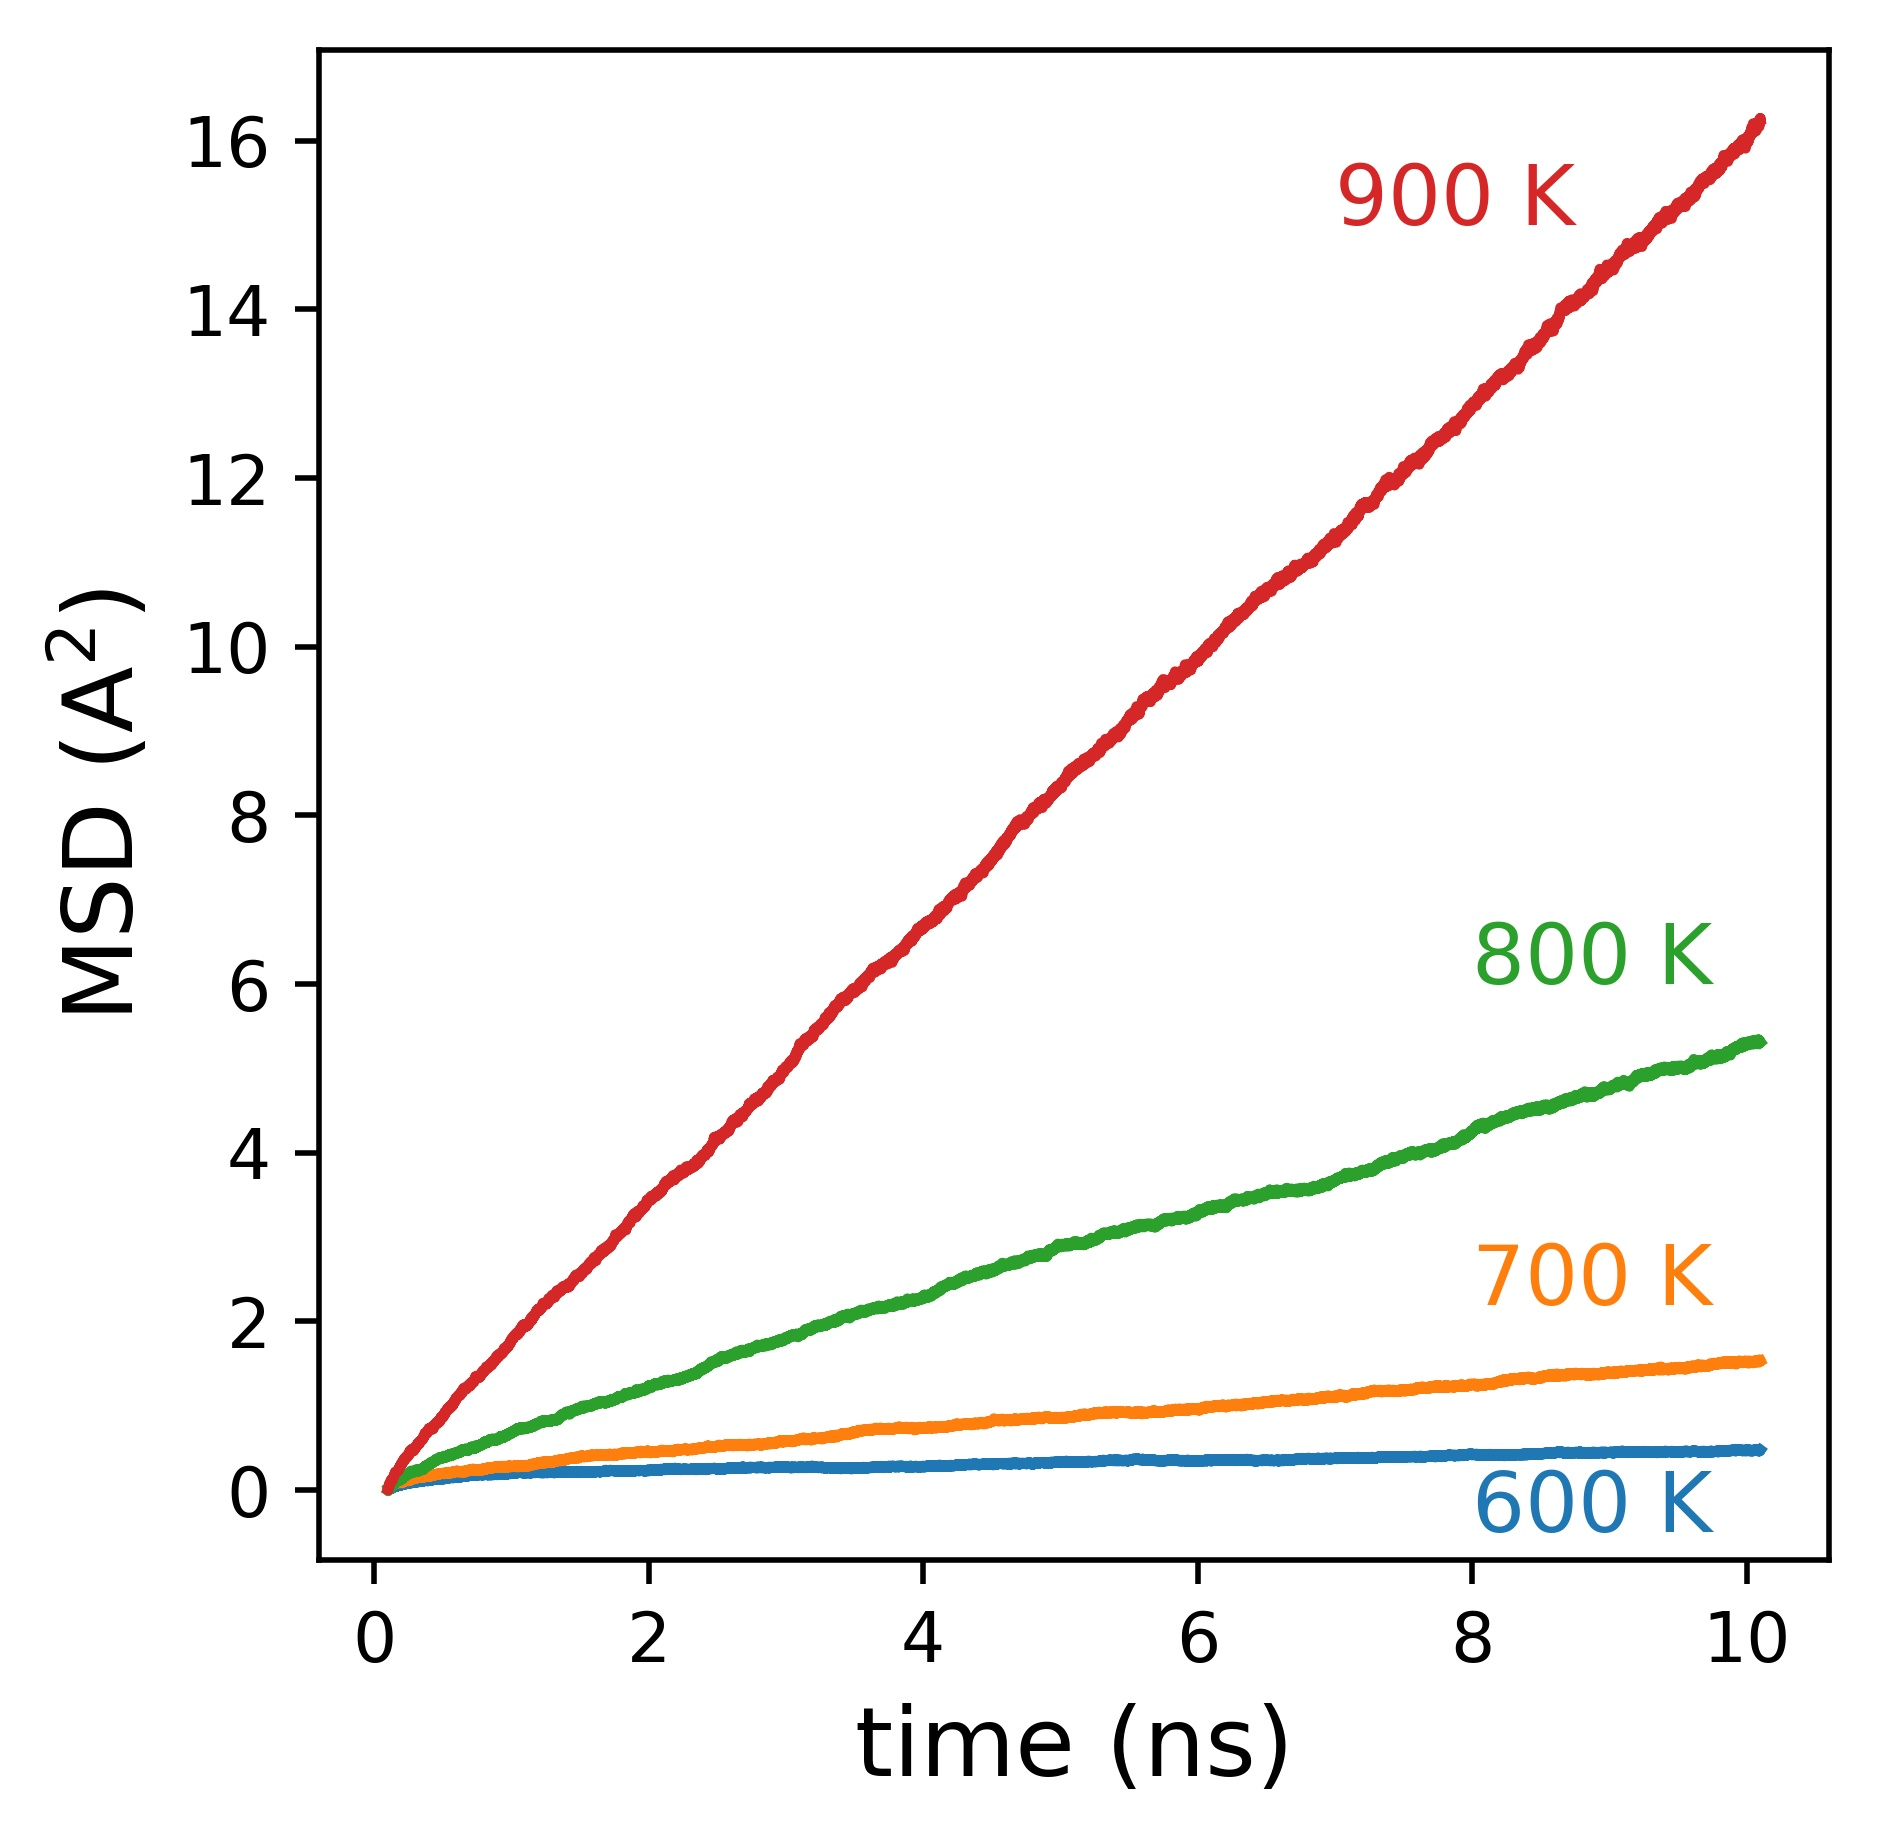
\includegraphics[height=5.4cm]{./figures/ca_msd.jpg}}
    \hspace{0.5cm}
    \subfloat[Al-doped, 1.2\%]{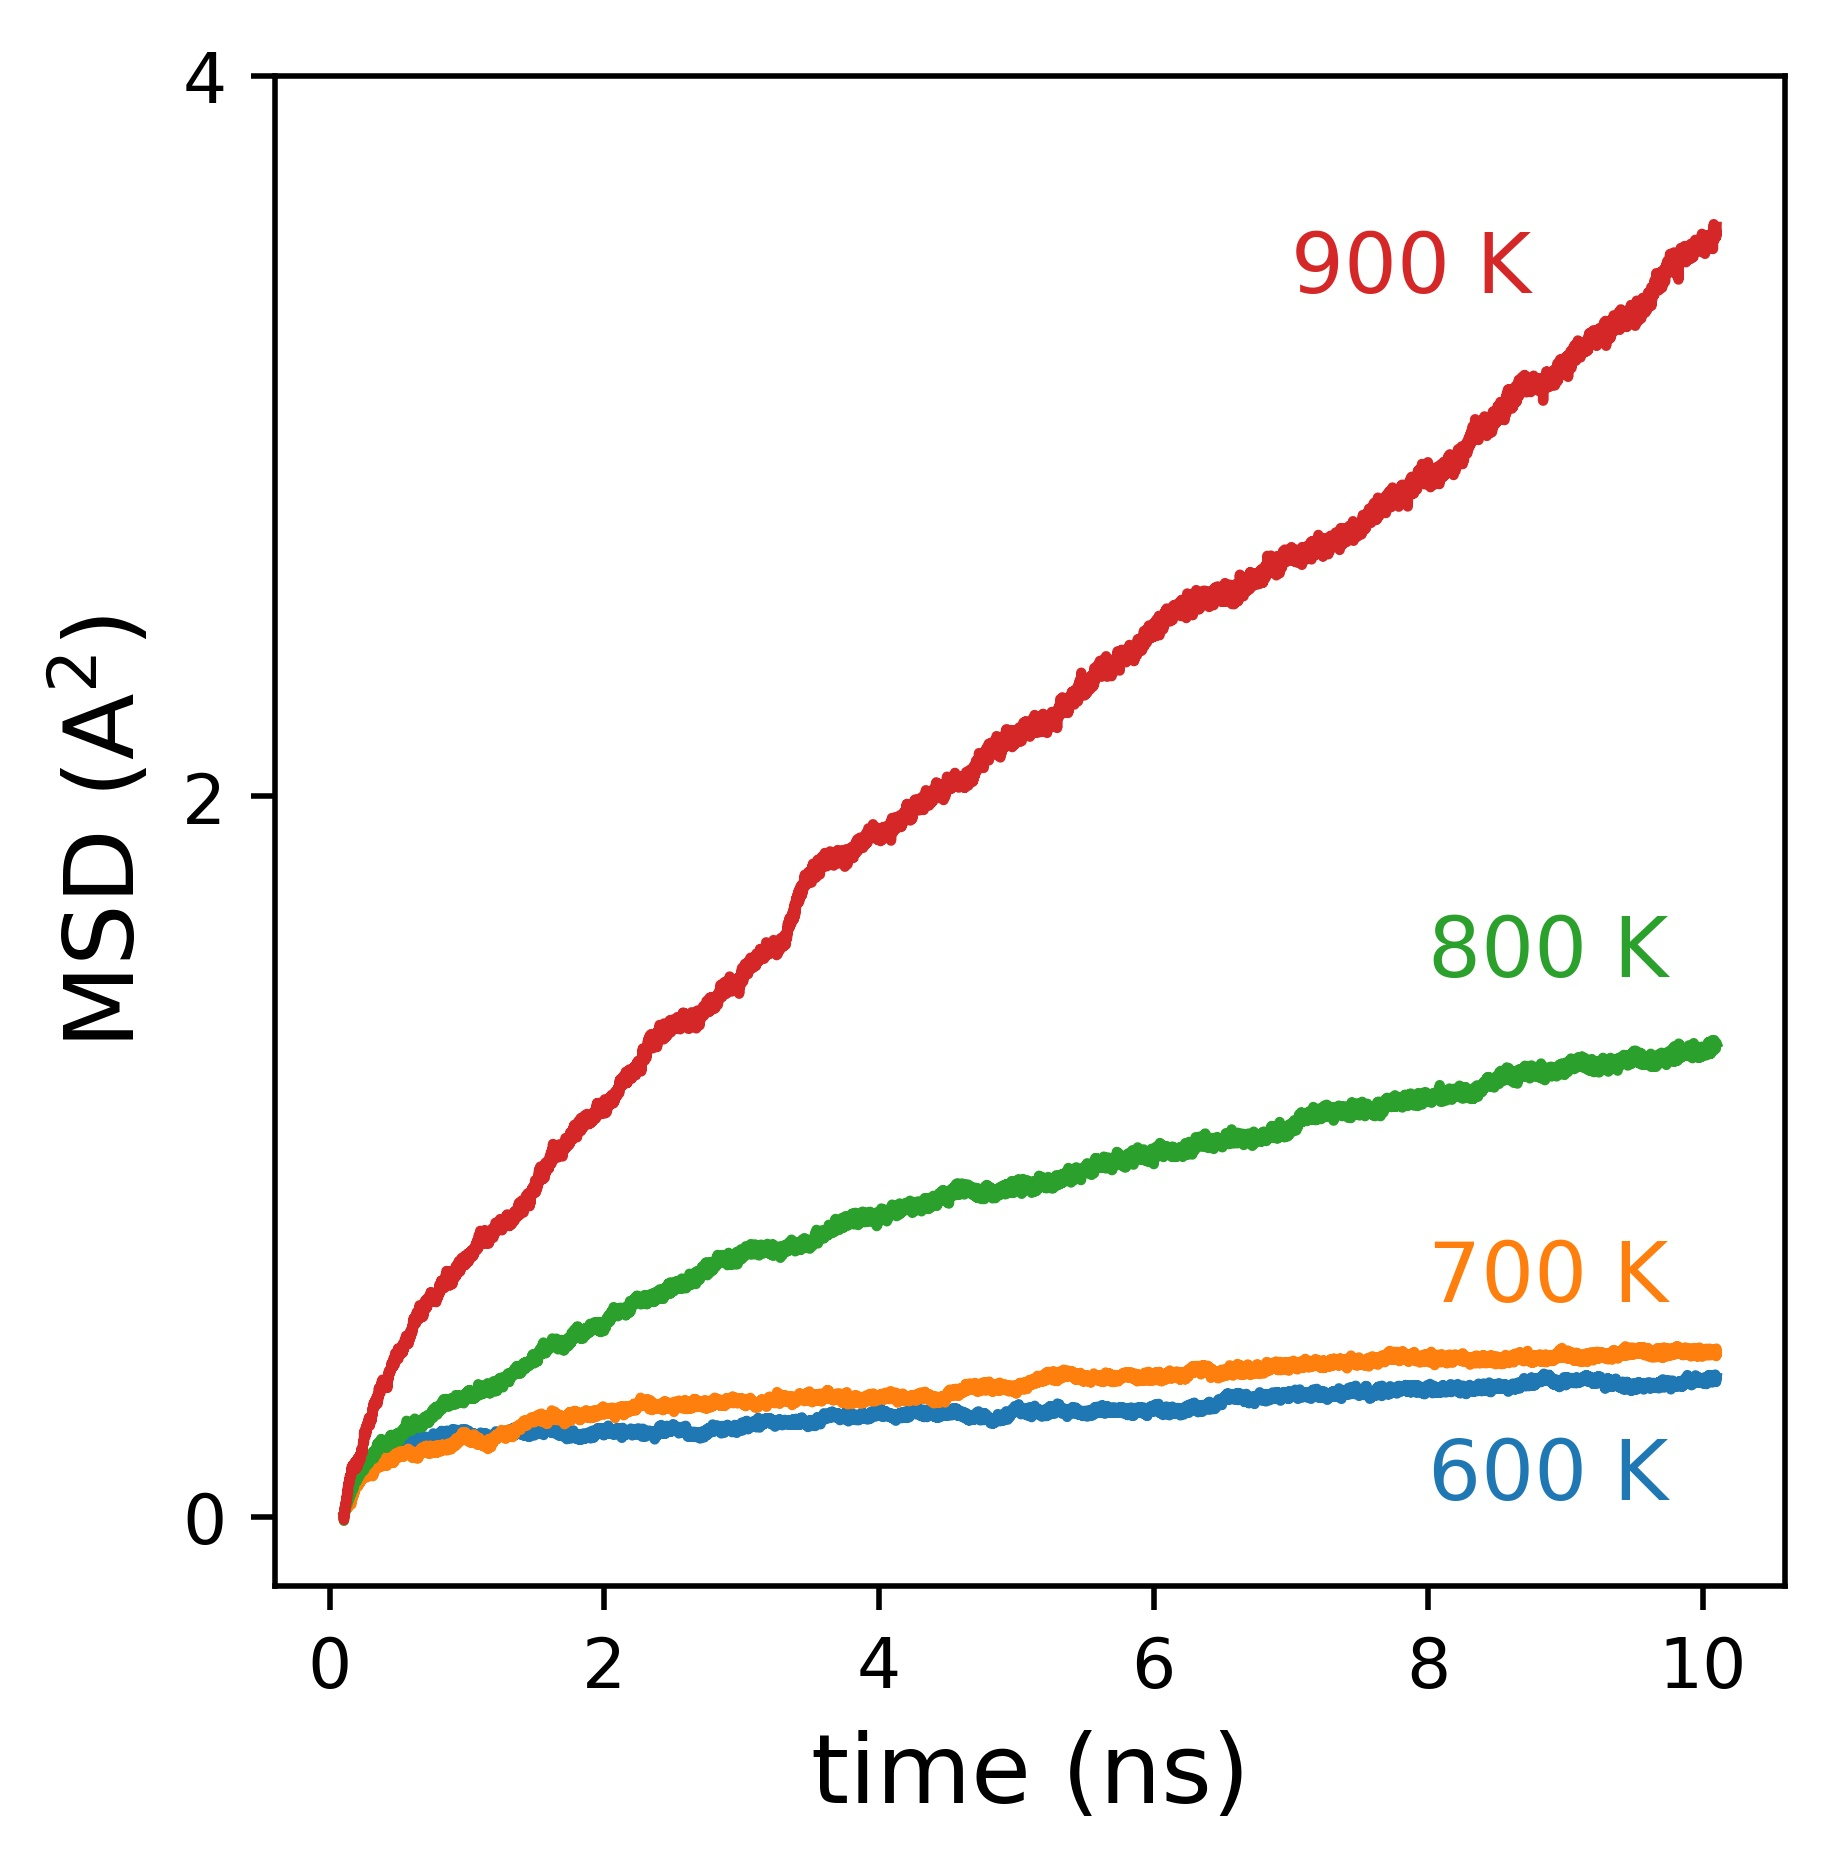
\includegraphics[height=5.4cm]{./figures/al_msd.jpg}}

    \subfloat[Ga-doped, 1.2\%]{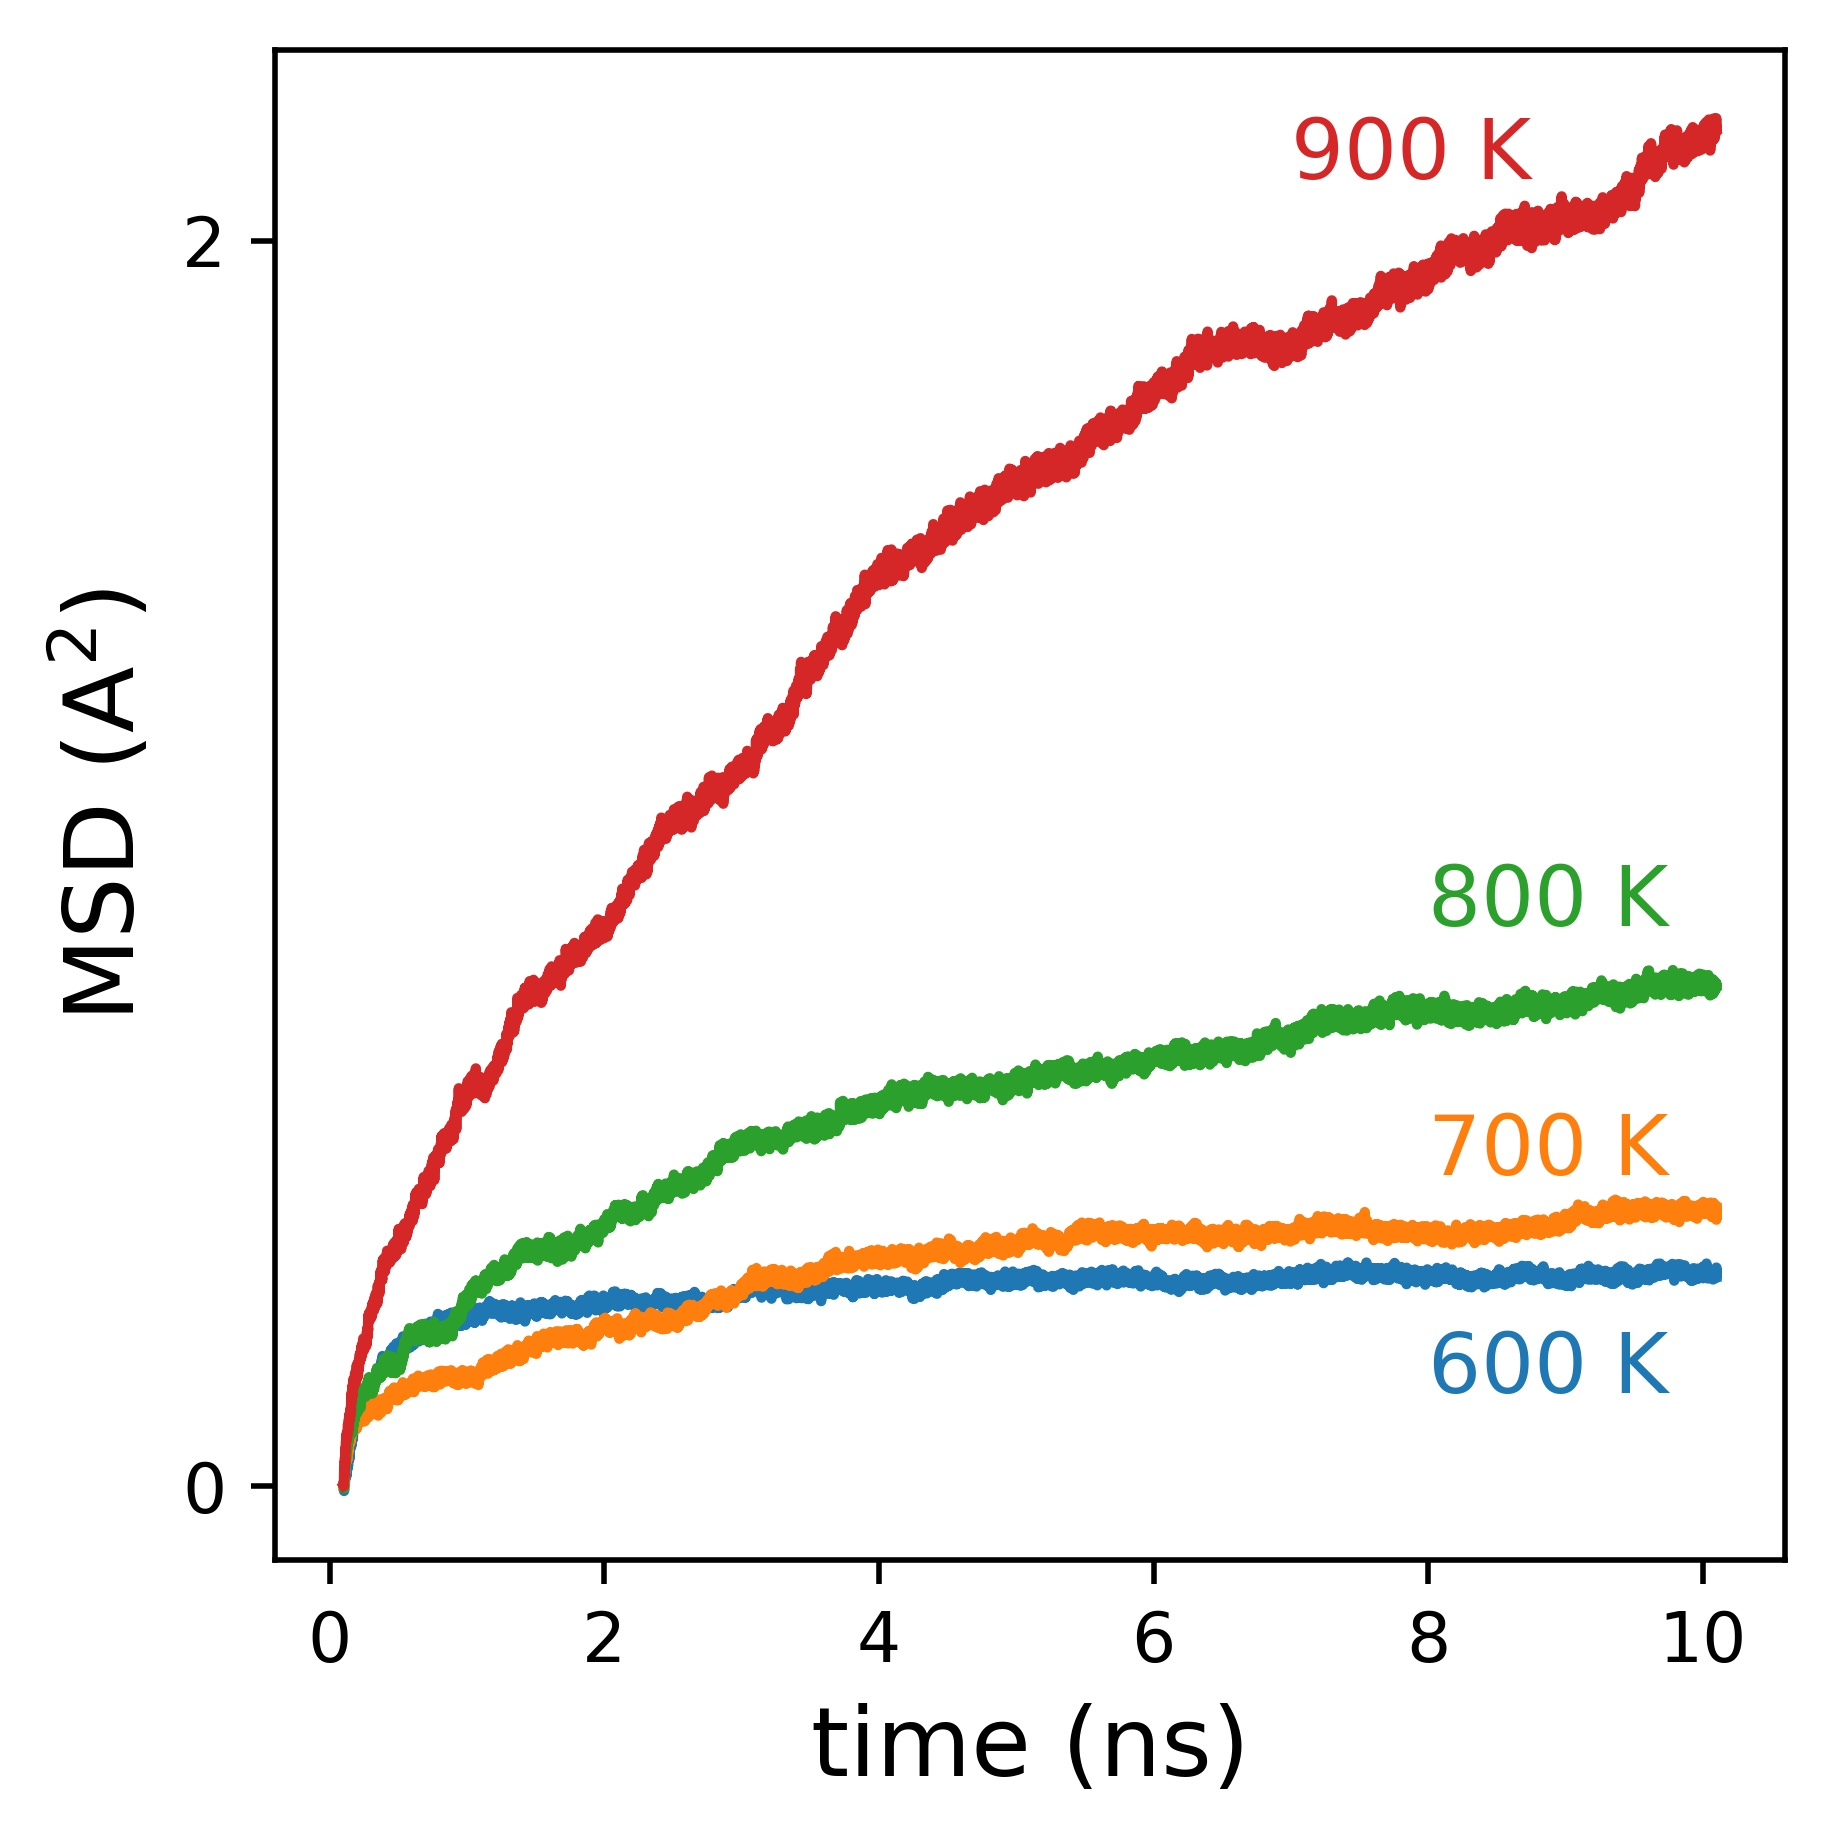
\includegraphics[height=5.4cm]{./figures/ga_msd.jpg}}
    \hspace{0.5cm}
    \subfloat[900 K]{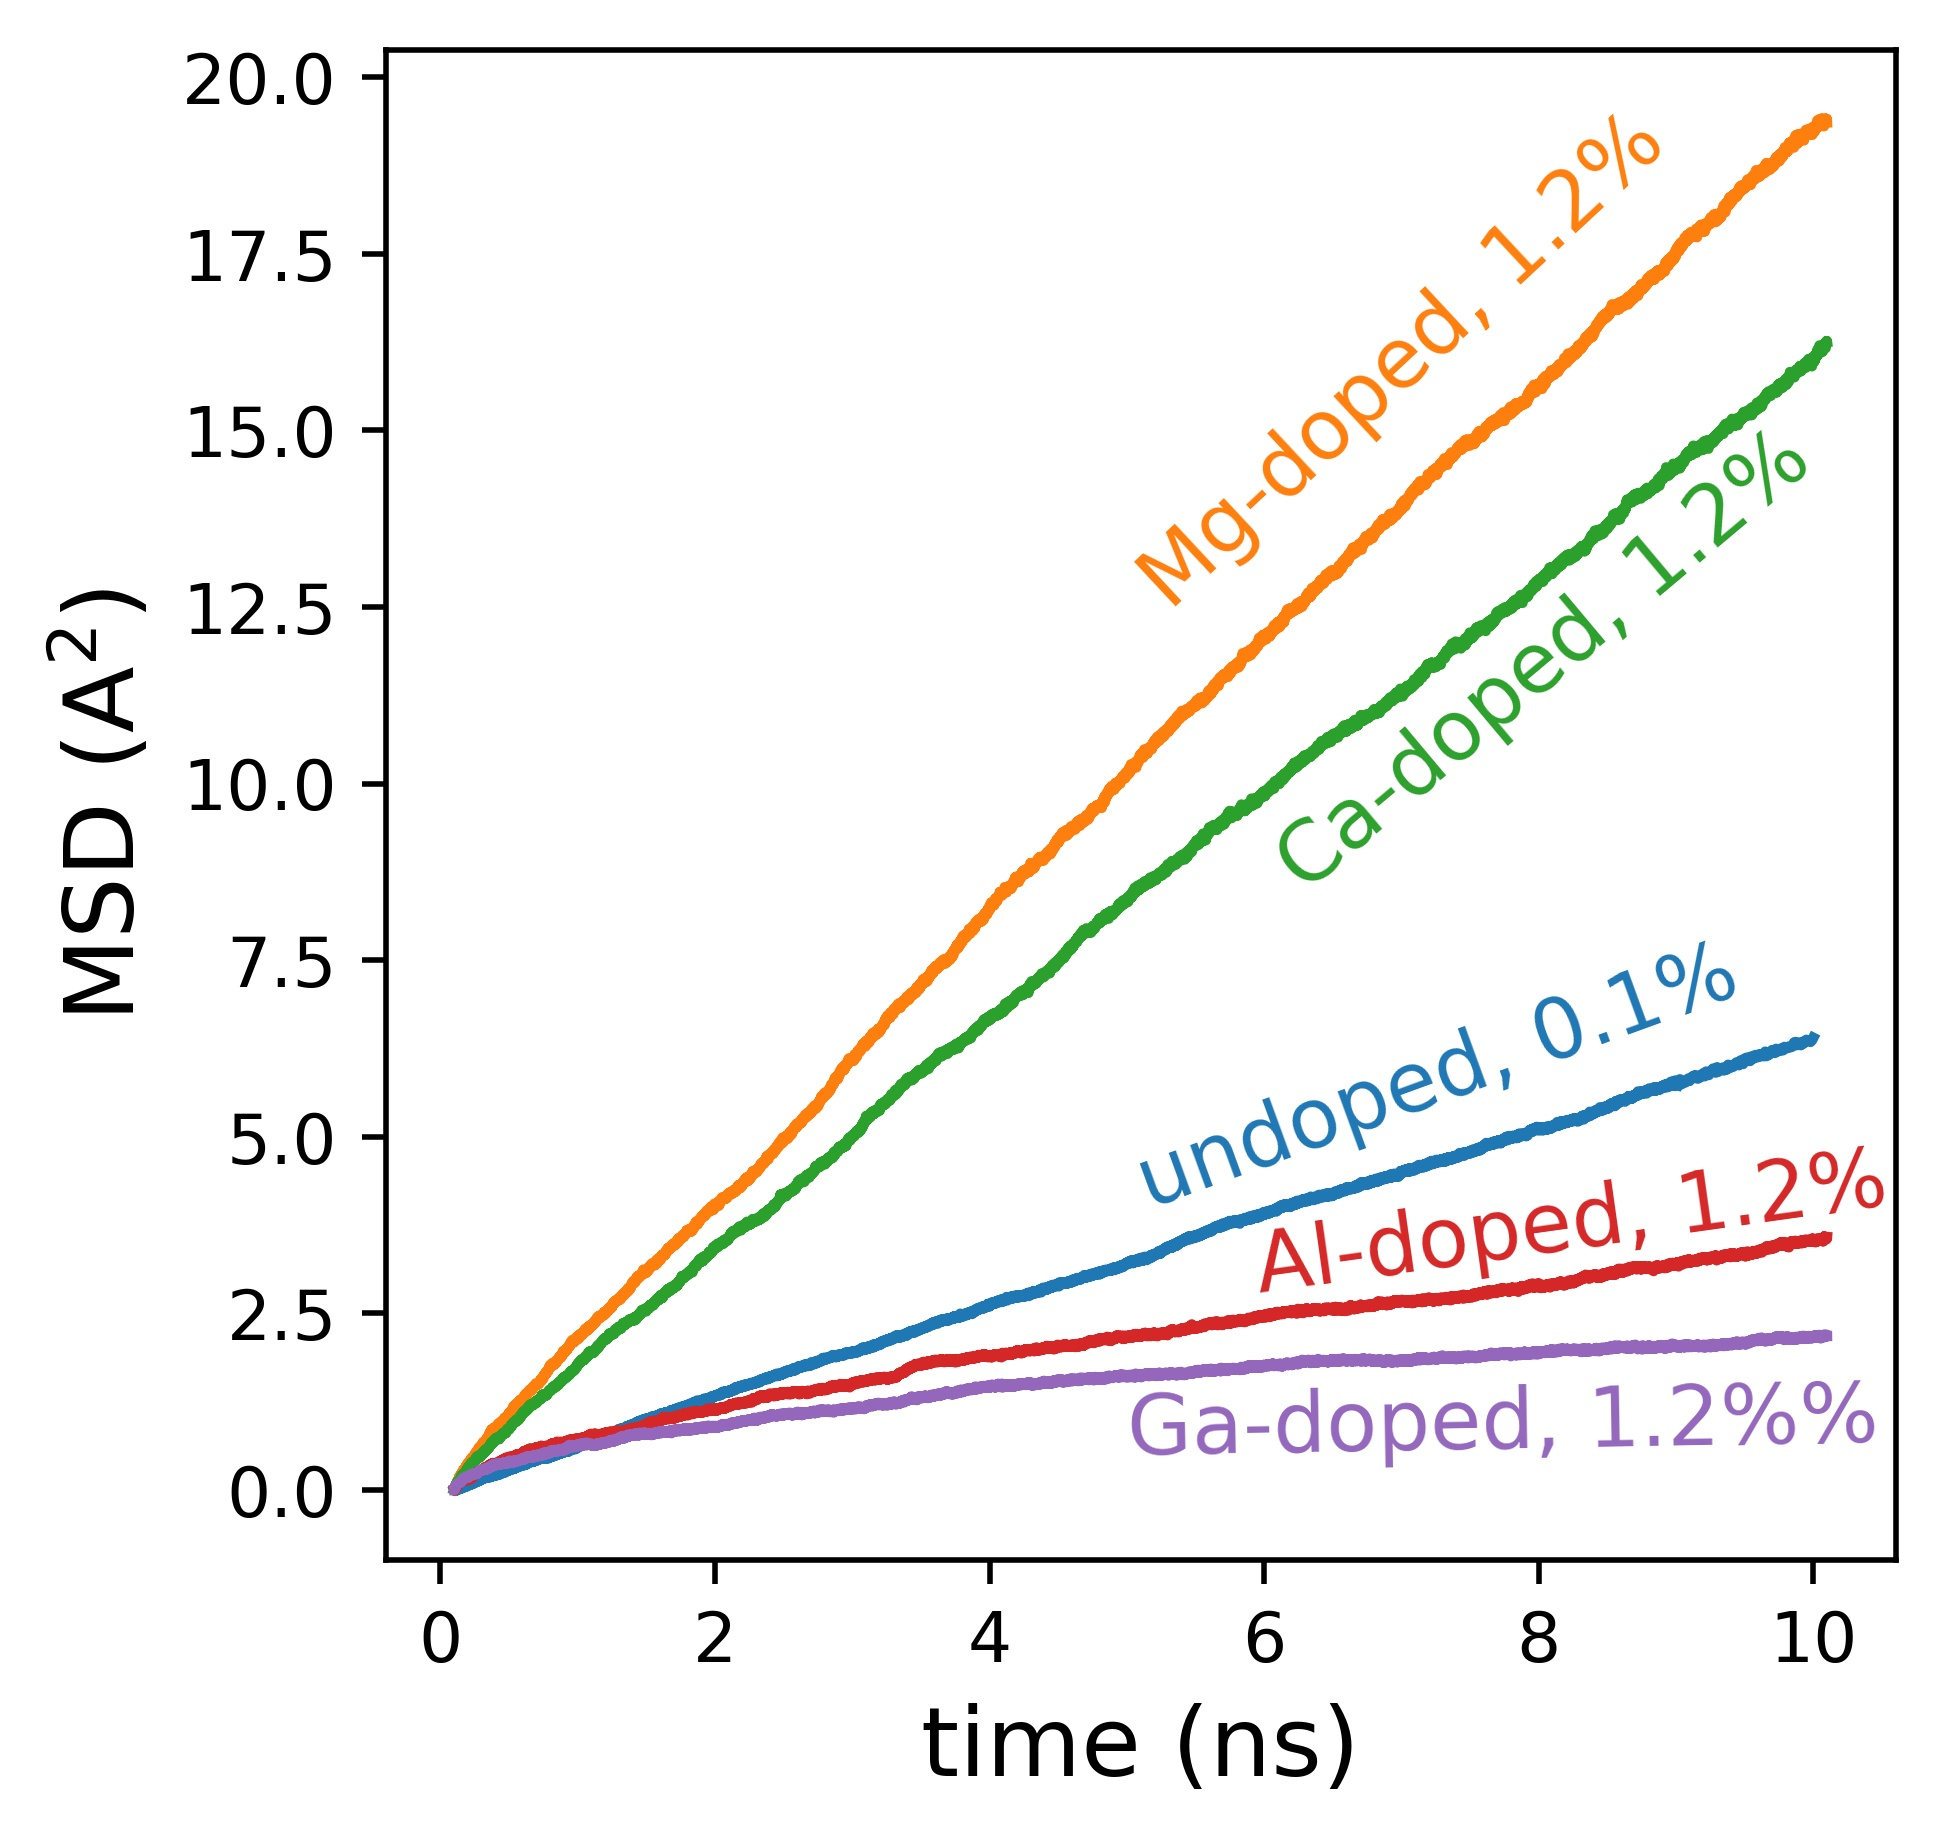
\includegraphics[height=5.6cm]{./figures/msd_900.jpg}}
    \caption{Representative examples of mean square displacement data for (a) undoped (b,c) divalent cation doped (d,e) trivalent cation doped \ch{Na3OCl} at four temperatures. Note different y-axis scales. (f) Comparison of the mean square displacement of the five different structures (a-e) at 900 K.}
    \label{msd}
\end{figure}

\begin{figure}[!ht]
\centering
    \sidesubfloat[]{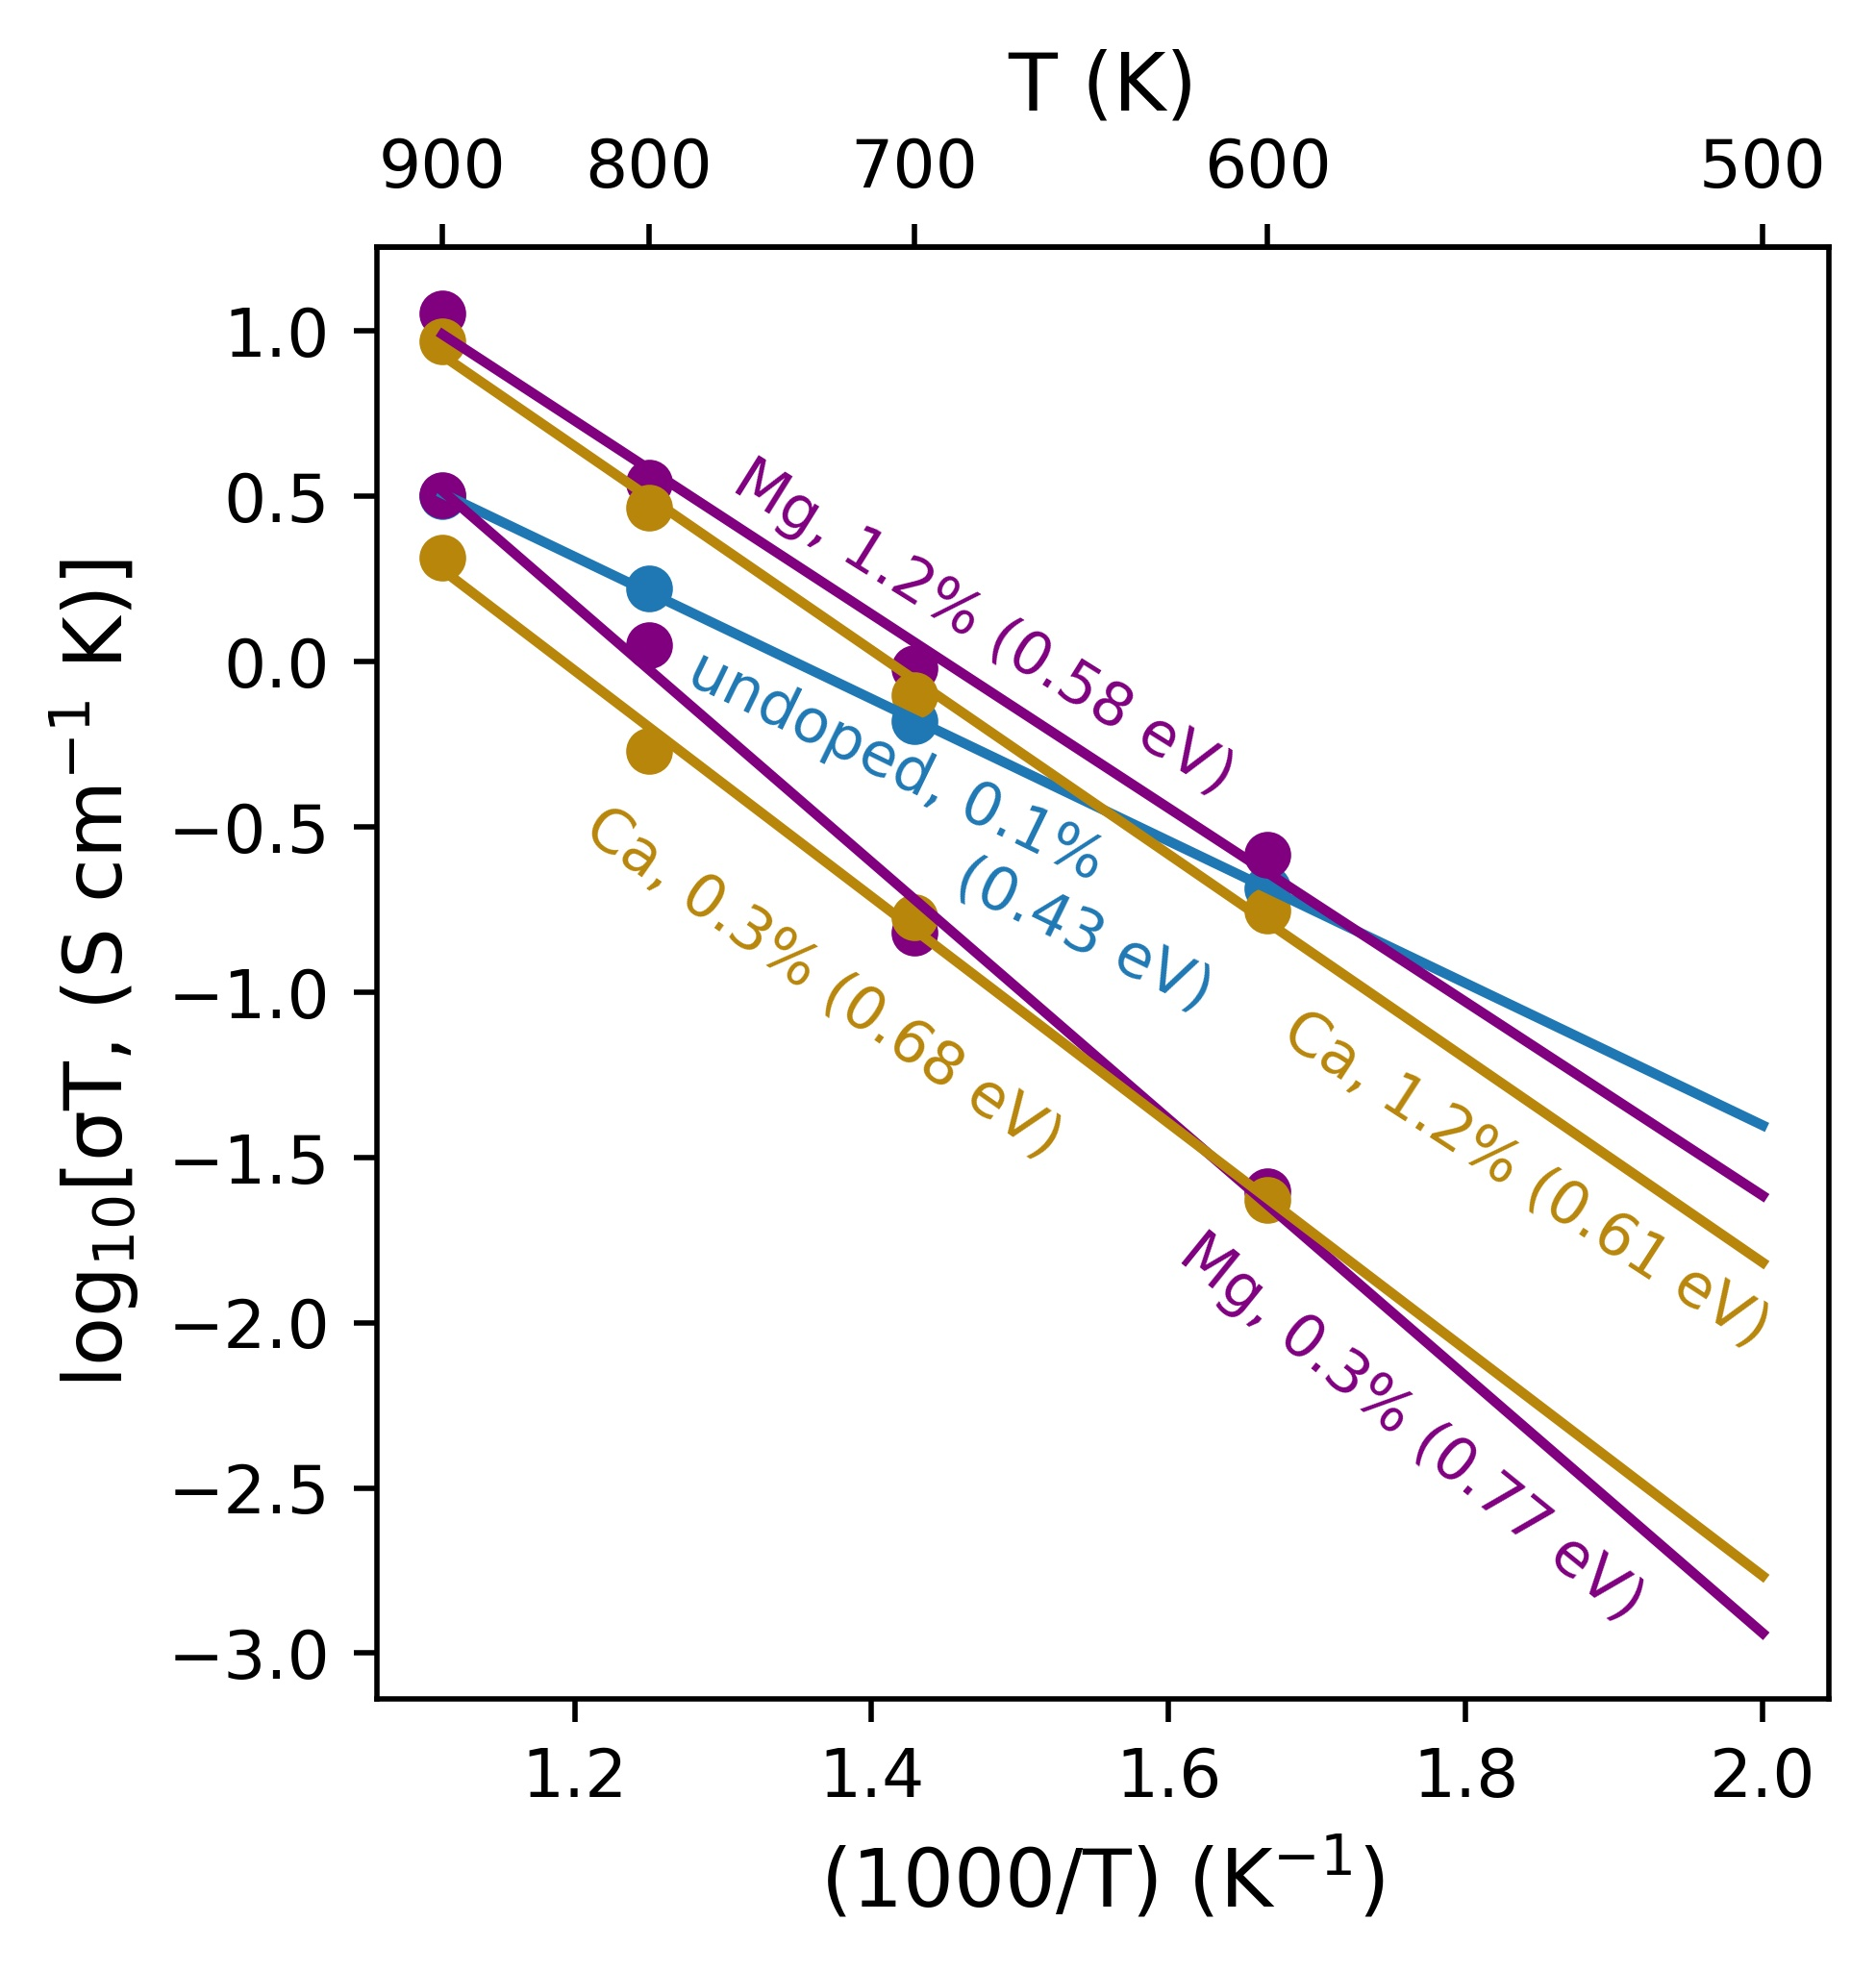
\includegraphics[width=9cm]{./figures/logconductivity_m2.jpg}\label{fig:conducivity2}}
    
    \sidesubfloat[]{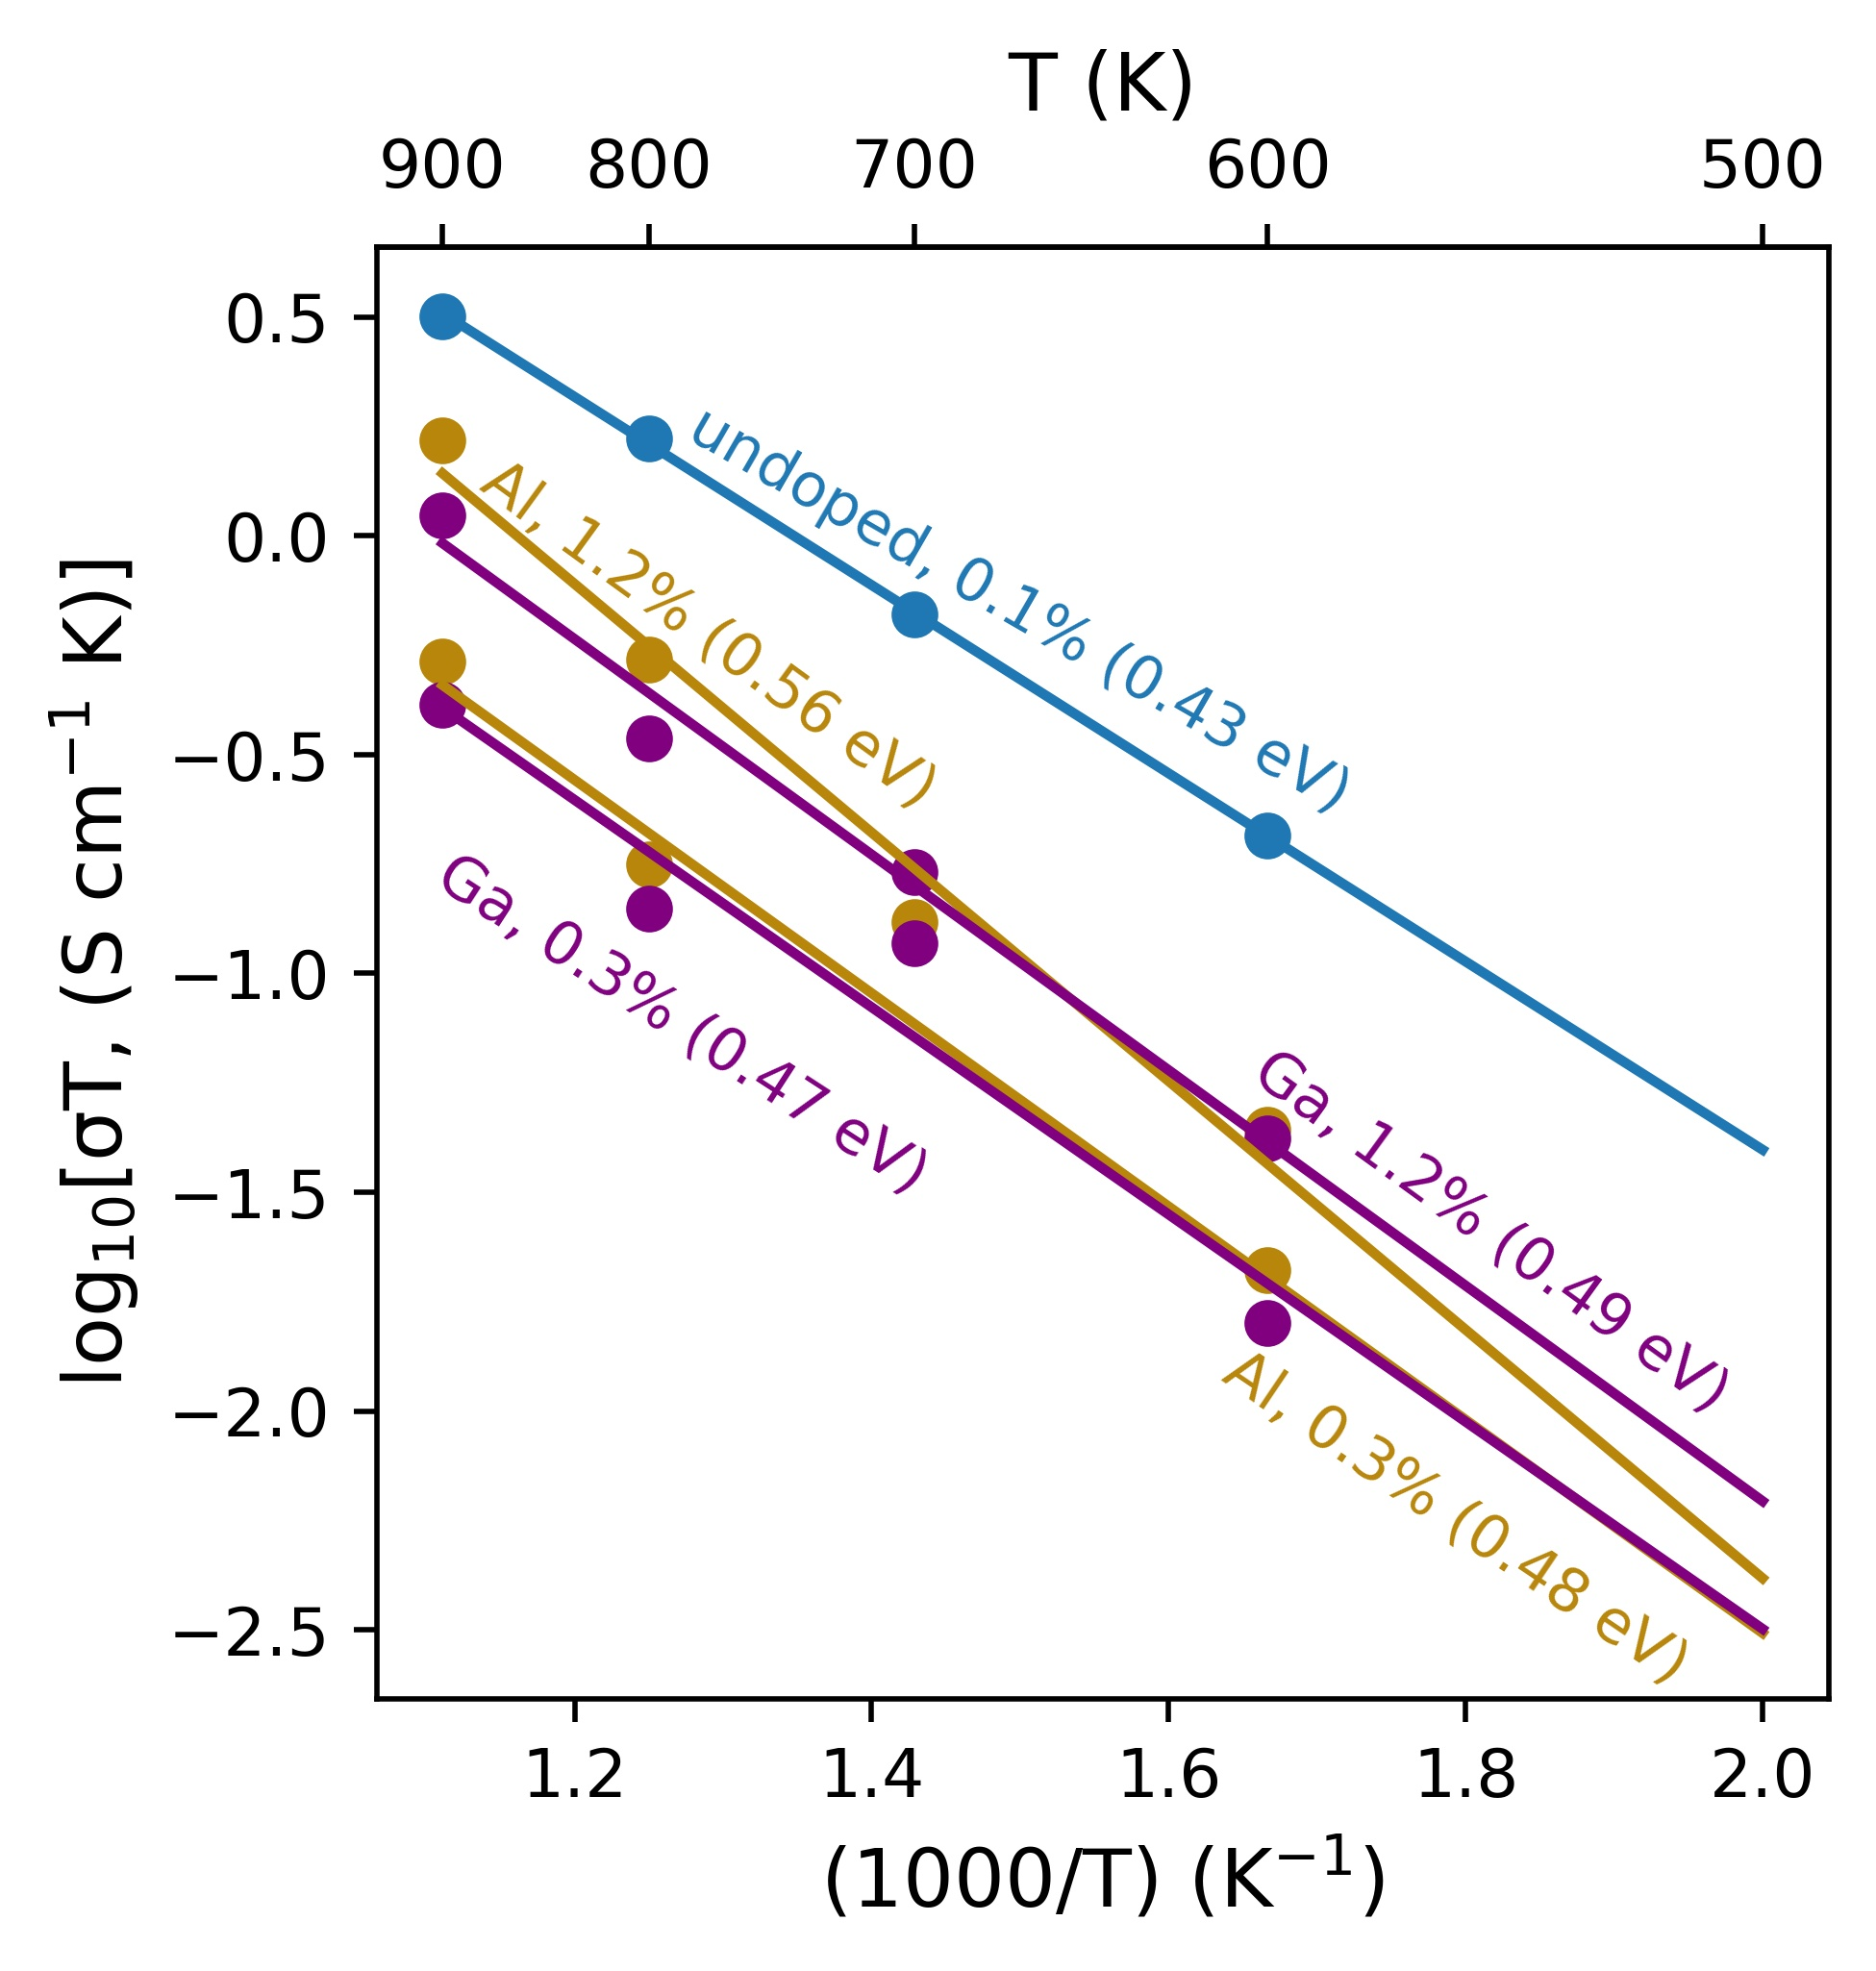
\includegraphics[width=9cm]{./figures/logconductivity_m3.jpg}\label{fig:conducivity3}}
    \caption{Temperature-dependent \ch{Na+} conductivities ($\mathrm{\sigma}$T) (a) Mg- and Ca-doped (b) Al-doped and Ga-doped \ch{Na3OCl} at two sodium vacancy concentrations compared to the undoped system.}
    \label{conductivity}
\end{figure}

\clearpage

From MD simulations we derived mean square displacement data (shown in Figure \ref{msd}), which allowed us the calculation of diffusion coefficients and ionic conductivities (as discussed in Chapter 2).
As expected the Na-ion diffusion increases with temperature.
Figure \ref{conductivity} shows an Arrhenius plot of the Na-ion conductivity over a wide temperature range for each system. 
The trends and magnitudes of the calculated ionic conductivities are consistent with experiment. 
The \ch{Na3OCl} material shows conductivities of 7.9 $\mathrm{\times \ 10^{-5} \ S \ cm^{-1}}$ (extrapolated at 500 K), in good agreement with experimental impedance spectroscopy measurements ($\mathrm{\sim}$ 4 $\mathrm{\times \ 10^{-5} \ S \ cm^{-1}}$).\cite{wang2015a}
Both Mg- and Ca-doping leads to a slight increase in ionic conductivity at higher dopant levels, with the latter having an activation barrier of 0.58 eV in agreement with experimental values ($\mathrm{\sim}$ 0.6 eV).\cite{wang2015a}
This concentration increase for Mg and Ca offsets the lower vacancy concentrations found in undoped \ch{Na3OCl}. 
The highest Na-ion conductivity is found for the Mg-doped (1.2\%) system. 
However, the Na-ion conductivities of the Al- and Ga-doped systems are lower than the undoped material, which may be related to greater defect clustering or binding factors, which we return to below. 

\begin{figure}
\centering
    \subfloat[]{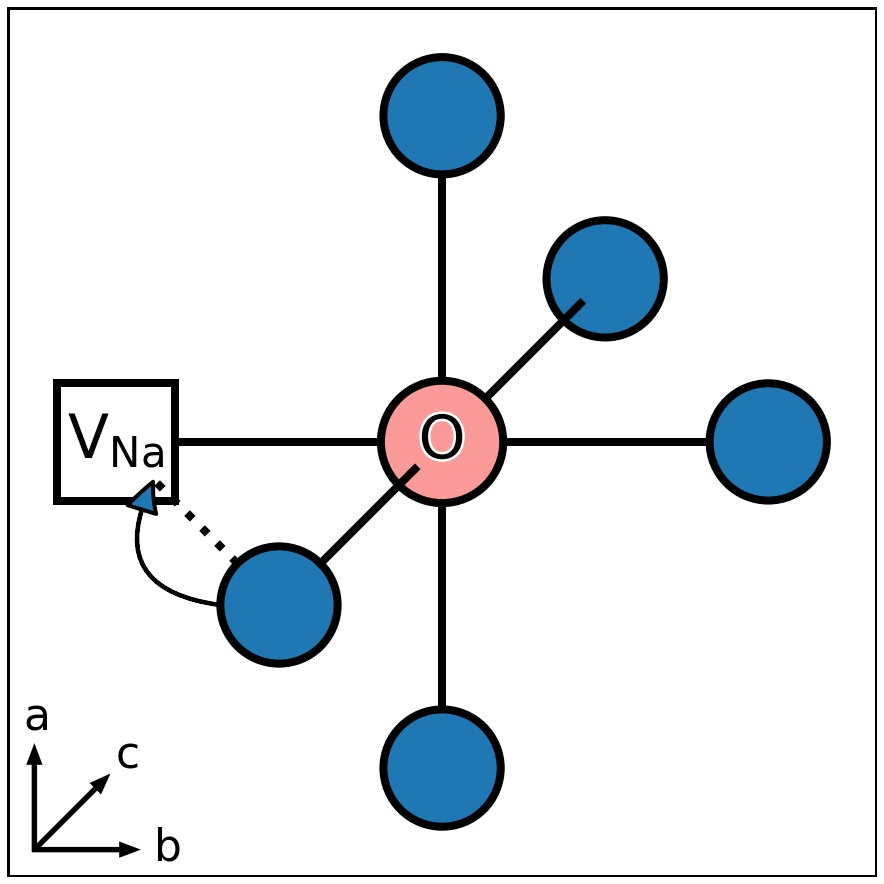
\includegraphics[width=4.3cm]{./figures/migration1.jpg}\label{fig:3d}}
    \hspace{0.5cm}
    \subfloat[]{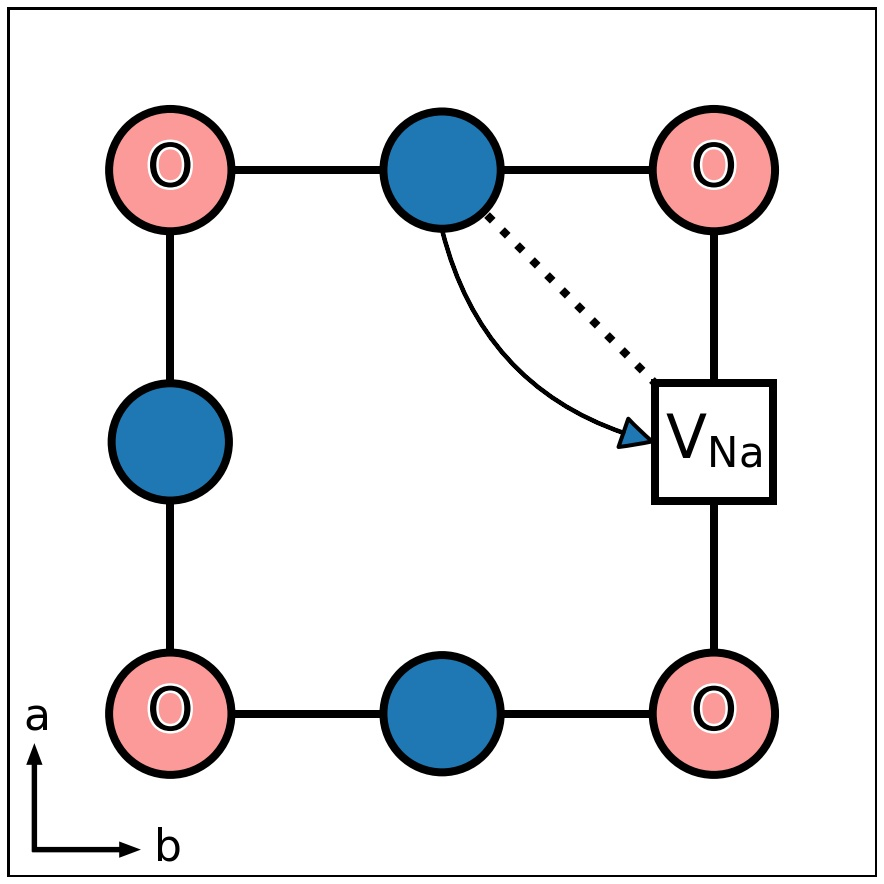
\includegraphics[width=4.3cm]{./figures/migration2.jpg}\label{fig:2d}}
    \hspace{0.5cm}
    \subfloat[]{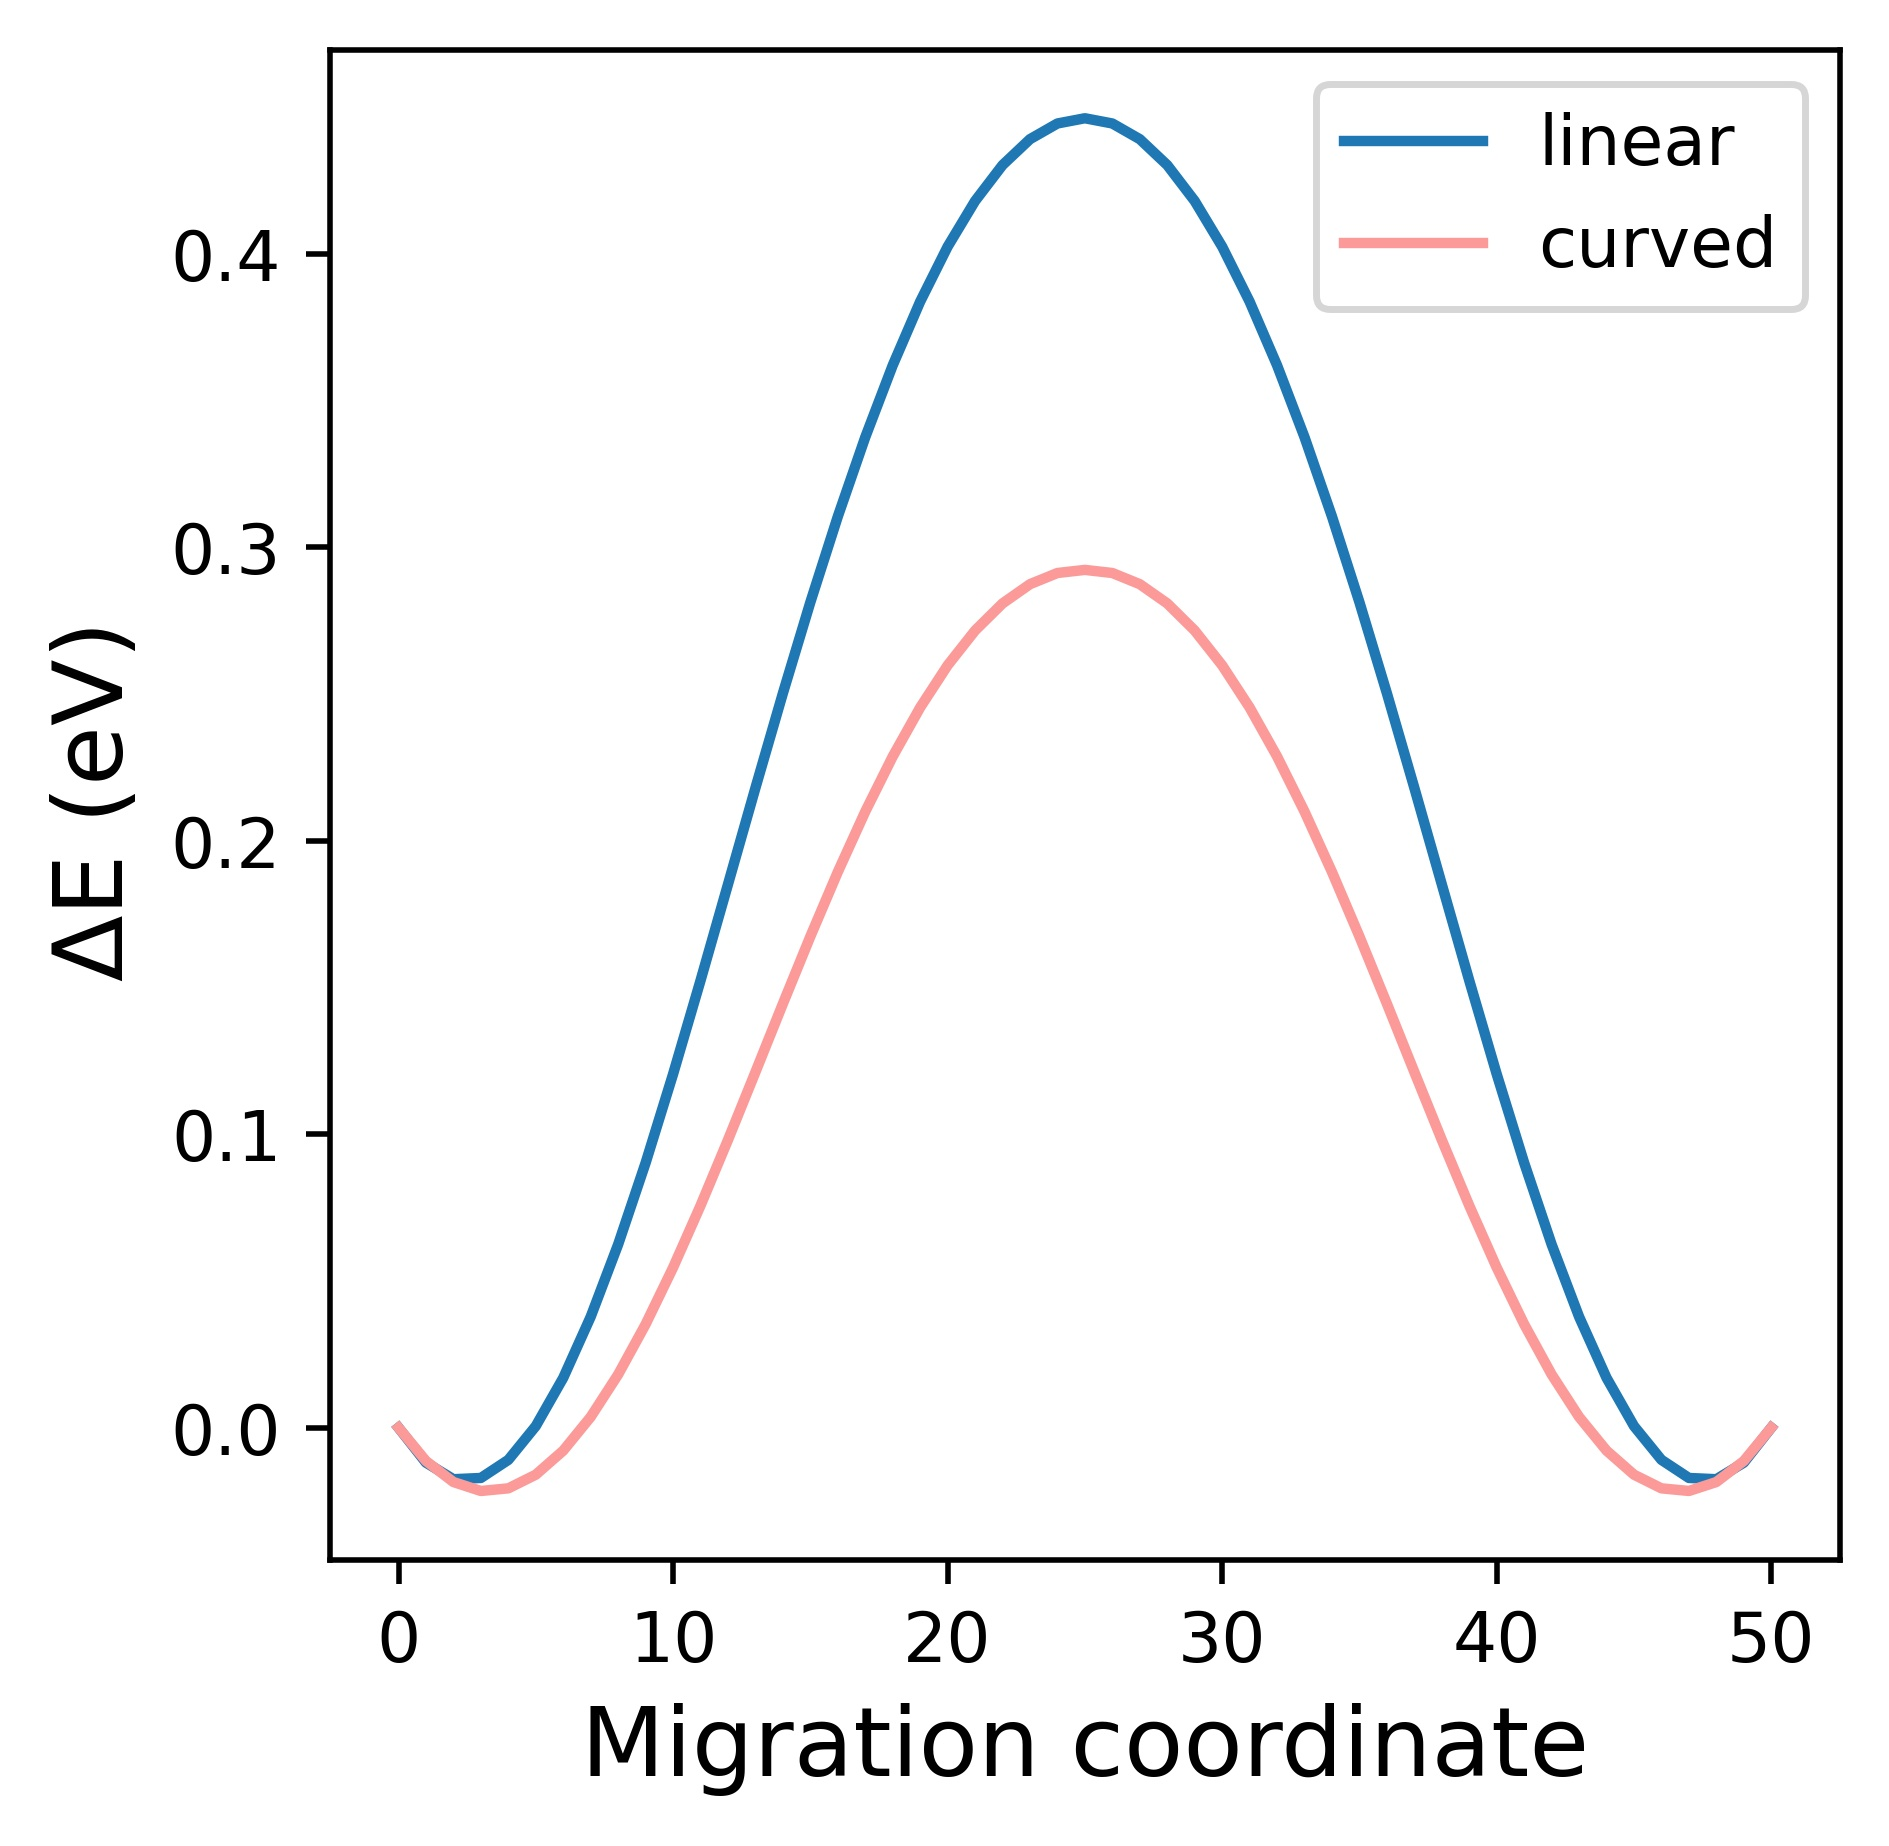
\includegraphics[width=4.3cm]{./figures/migration.jpg}\label{fig:energy}}
\caption{Schematic of the curved migration path for the \ch{Na+} vacancy migration (a) along the \ch{ONa6} octahedron edge (b) looking down the (1 0 0) plane. (c) Energy profile for Na ion migration along the straight (blue) and curved (red) migration pathways of the \ch{ONa6} octahedra in \ch{Na3OCl}.}
\label{migration}
\end{figure}

It is sometimes assumed that the migrating ion takes the shortest path between adjacent sites, i.e., a direct linear jump. 
However, our simulations identify curved paths between adjacent Na sites (Figure \ref{migration}), whose profile shows a lower activation barrier than the linear migration path.
It is worth noting that analogous, curved migration paths were first predicted from our atomistic simulation studies of Li-ion migration in \ch{LiFePO4},\cite{islam2005} and oxide-ion migration in perovskite oxides, such as \ch{LaGaO3},\cite{khan1998} which were subsequently confirmed by experimental studies using neutron diffraction maximum entropy methods.\cite{nishimura2008, yashima2003}

\begin{figure}
\centering
    \subfloat[]{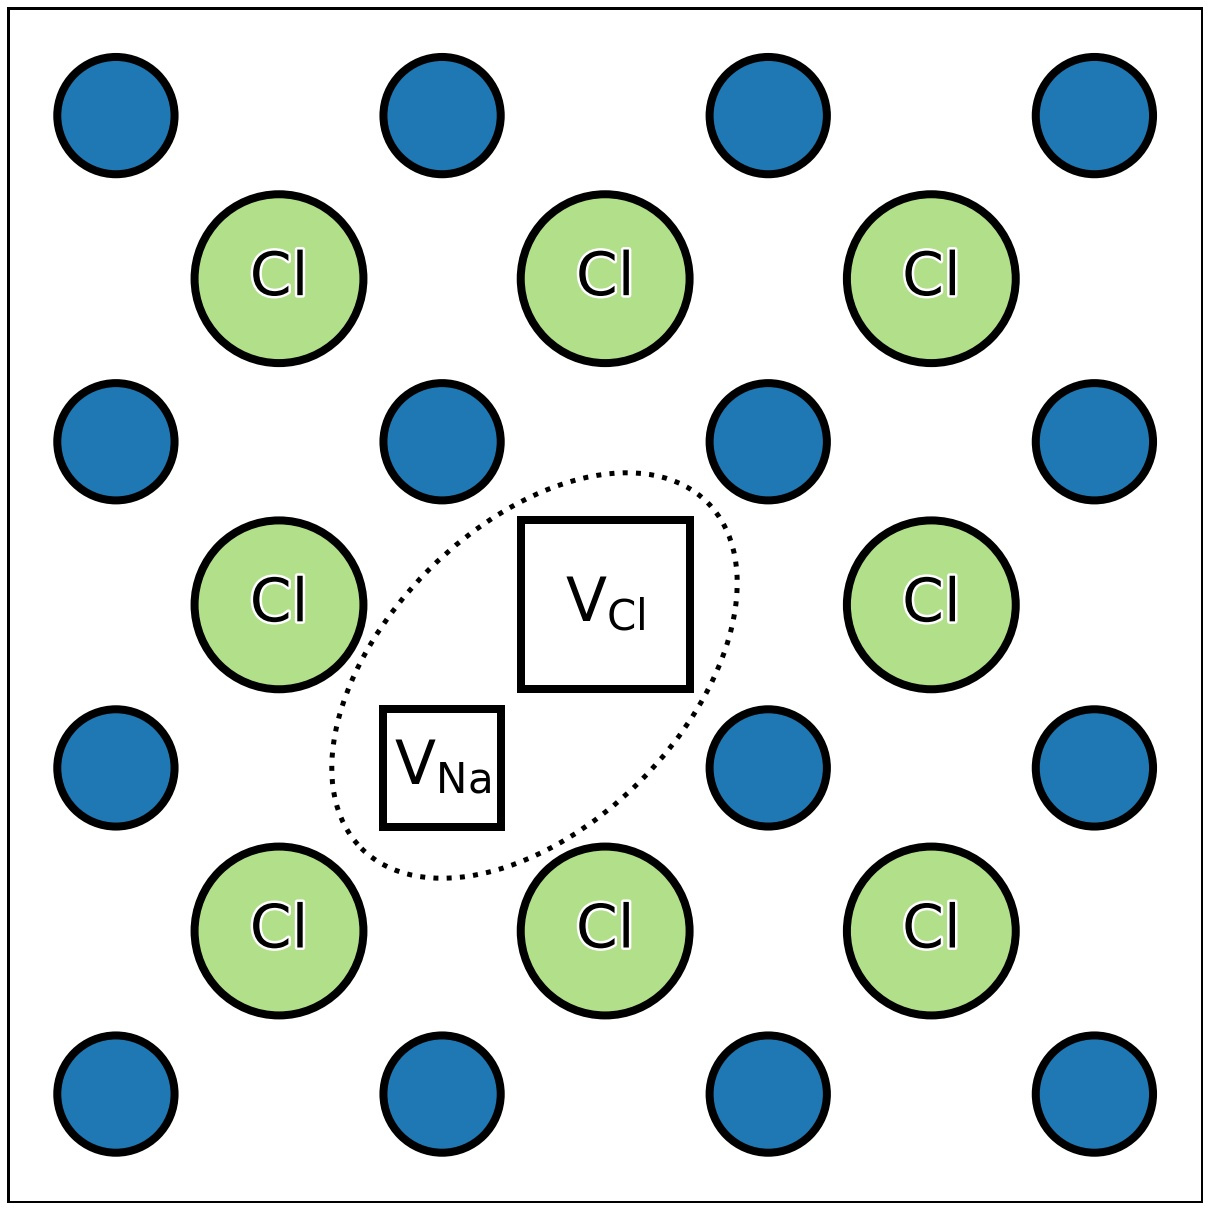
\includegraphics[width=5cm]{./figures/schottky.jpg}\label{fig:schottky}}
    \hspace{1cm}
    \subfloat[]{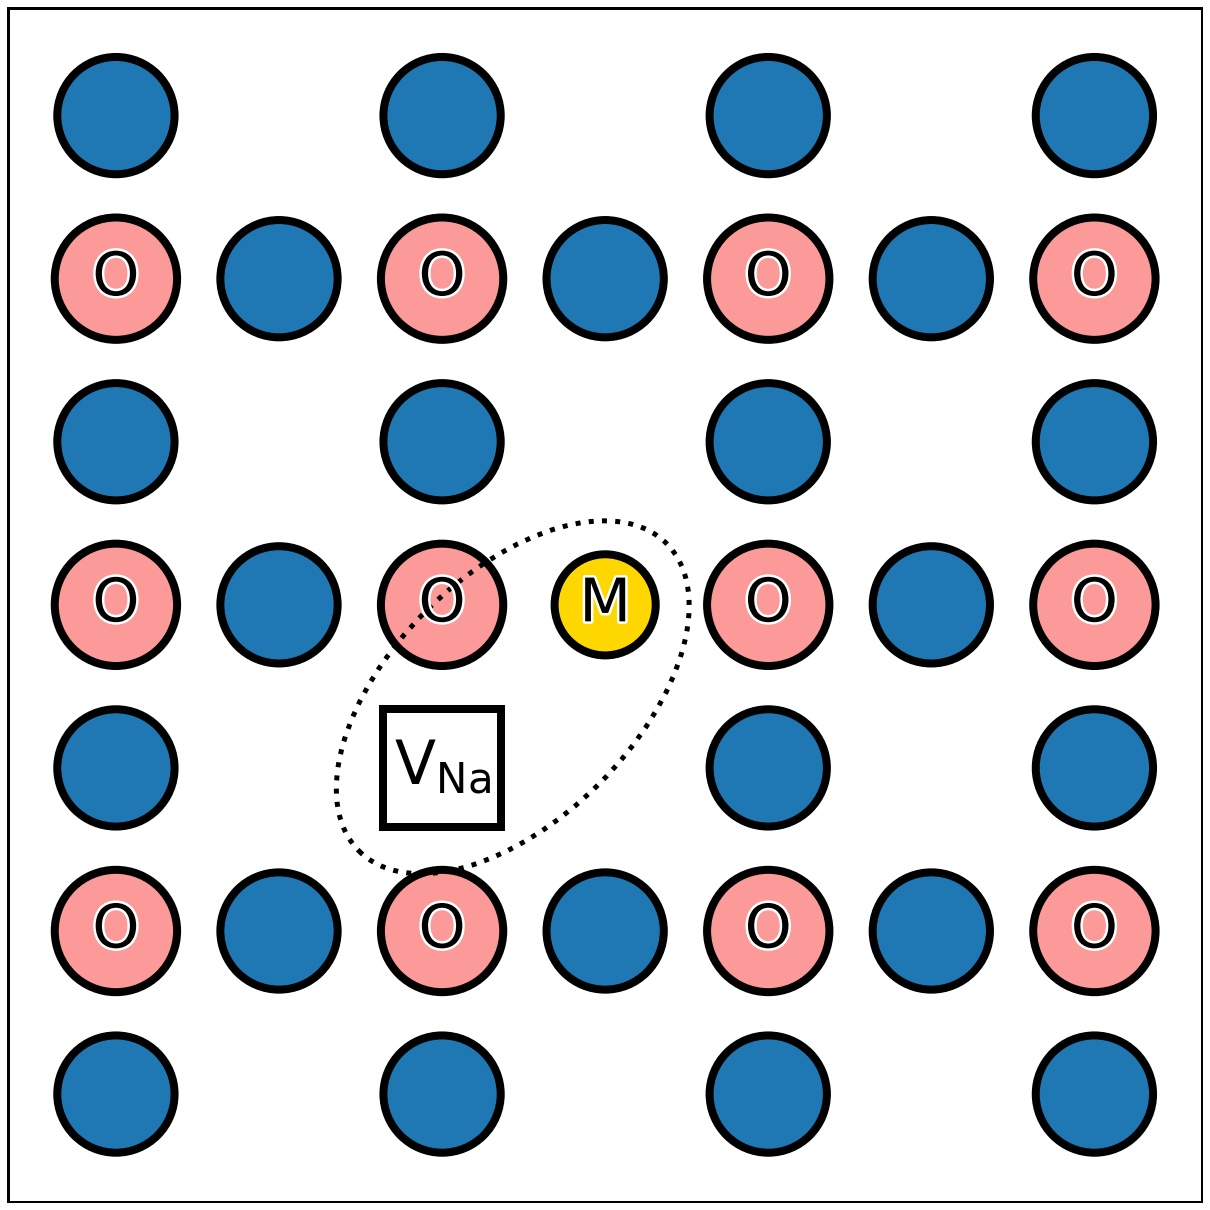
\includegraphics[width=5cm]{./figures/doping_pic.jpg}\label{fig:dopant}}
    
    \subfloat[]{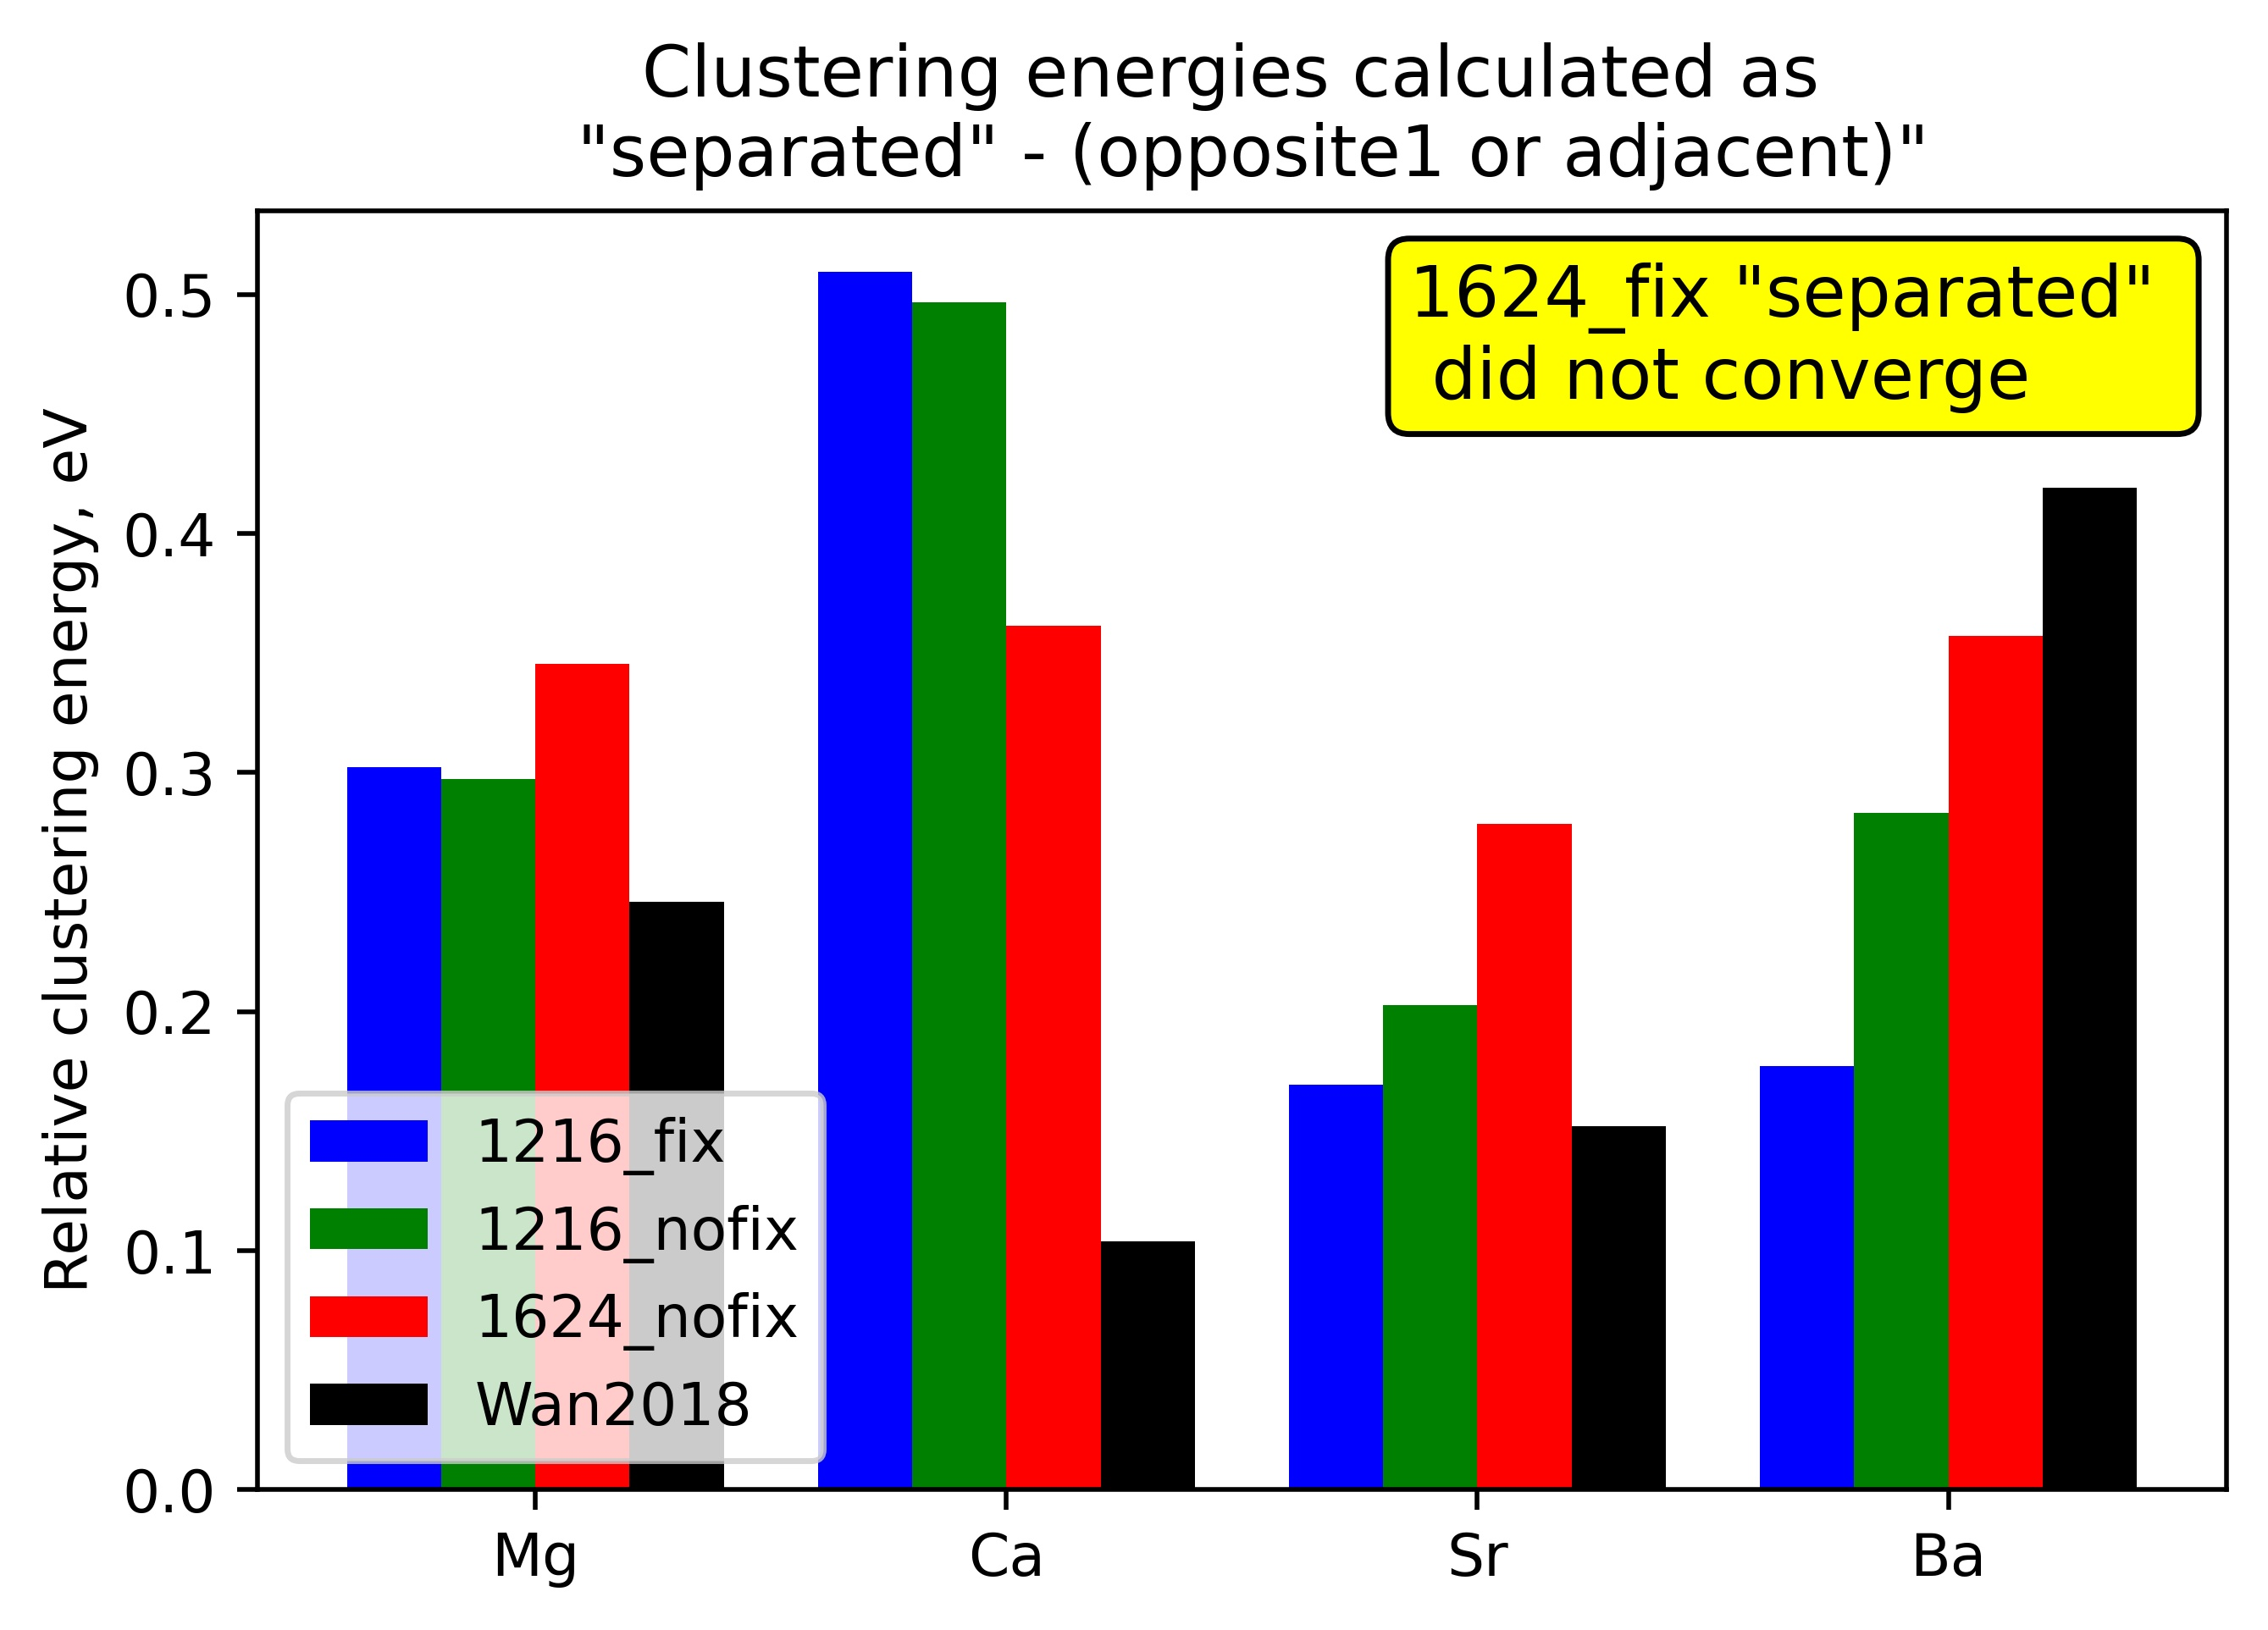
\includegraphics[width=9cm]{./figures/clustering.jpg}\label{fig:clustering}}
\caption{Defect clustering in \ch{Na3OCl} (a) undoped structure with sodium and chloride vacancies; (b) doped structures with a sodium vacancy and and a dopant ion. (c) Binding energies for pair clusters.}
\label{clustering}
\end{figure}

It is well known that charged point defects can associate to form localised clusters, which can inhibit ion transport. 
However, the experimental characterisation of such defect clusters can be difficult. 
Simulations were performed to determine the binding energies of dopant-vacancy pairs in \ch{Na3OCl}. 
Figure \ref{clustering} show the configurations of dopant-vacancy clusters, as well as the Na/Cl vacancy pair (from the NaCl Schottky-type defect). 
The binding energy for the defect clusters can be derived from the difference in the calculated energy of the defect pair cluster and the energy of the individual isolated defects that make up the cluster.

\begin{equation}
    E_{bind} = E_{cluster} - \sum E_{isolated}
\end{equation}

\noindent
For example, the binding energy of a \ch{Mg^{2+}} dopant and a Na vacancy is given by:

\begin{equation}
    E_{bind} = E(\ch{Mg_{Na}^{$\bullet$}}-\ch{V_{Na}^{$\prime$}}) - \Big\{ E(\ch{Mg_{Na}^{$\bullet$}}) + E(\ch{V_{Na}^{$\prime$}}) \Big\}
\end{equation}

\noindent
A negative binding energy value indicates that the cluster is stable with respect to the isolated component defects. 

The resulting binding energies are shown in Figure \ref{fig:clustering} with two main features identified. 
First, \ch{Mg^{2+}} has the smallest binding energy, suggesting that at the dilute limit, Na vacancies are weakly bound to Mg dopants, with a similar binding energy to the undoped system. 
This indicates that dopant-vacancy interactions will not significantly reduce the Na-ion mobility of Mg-doped \ch{Na3OCl}. 
Second, all other dopants show high binding energies ($>0.5$ eV) with the largest value for \ch{Al^{3+}}, which could lead to ‘trapping’ of the migrating Na vacancies and hinder Na-ion conductivity in these materials. 
These results suggest clustering of Na vacancies and dopant ions rather than a random point defect distribution. 
The differences in Na-ion conductivity found between doped materials (Figure \ref{conductivity}) can be largely rationalised by Na vacancy trapping effects inhibiting sodium mobility in systems with high binding energies. 

\begin{figure}[htbp]
\centering
    \sidesubfloat[]{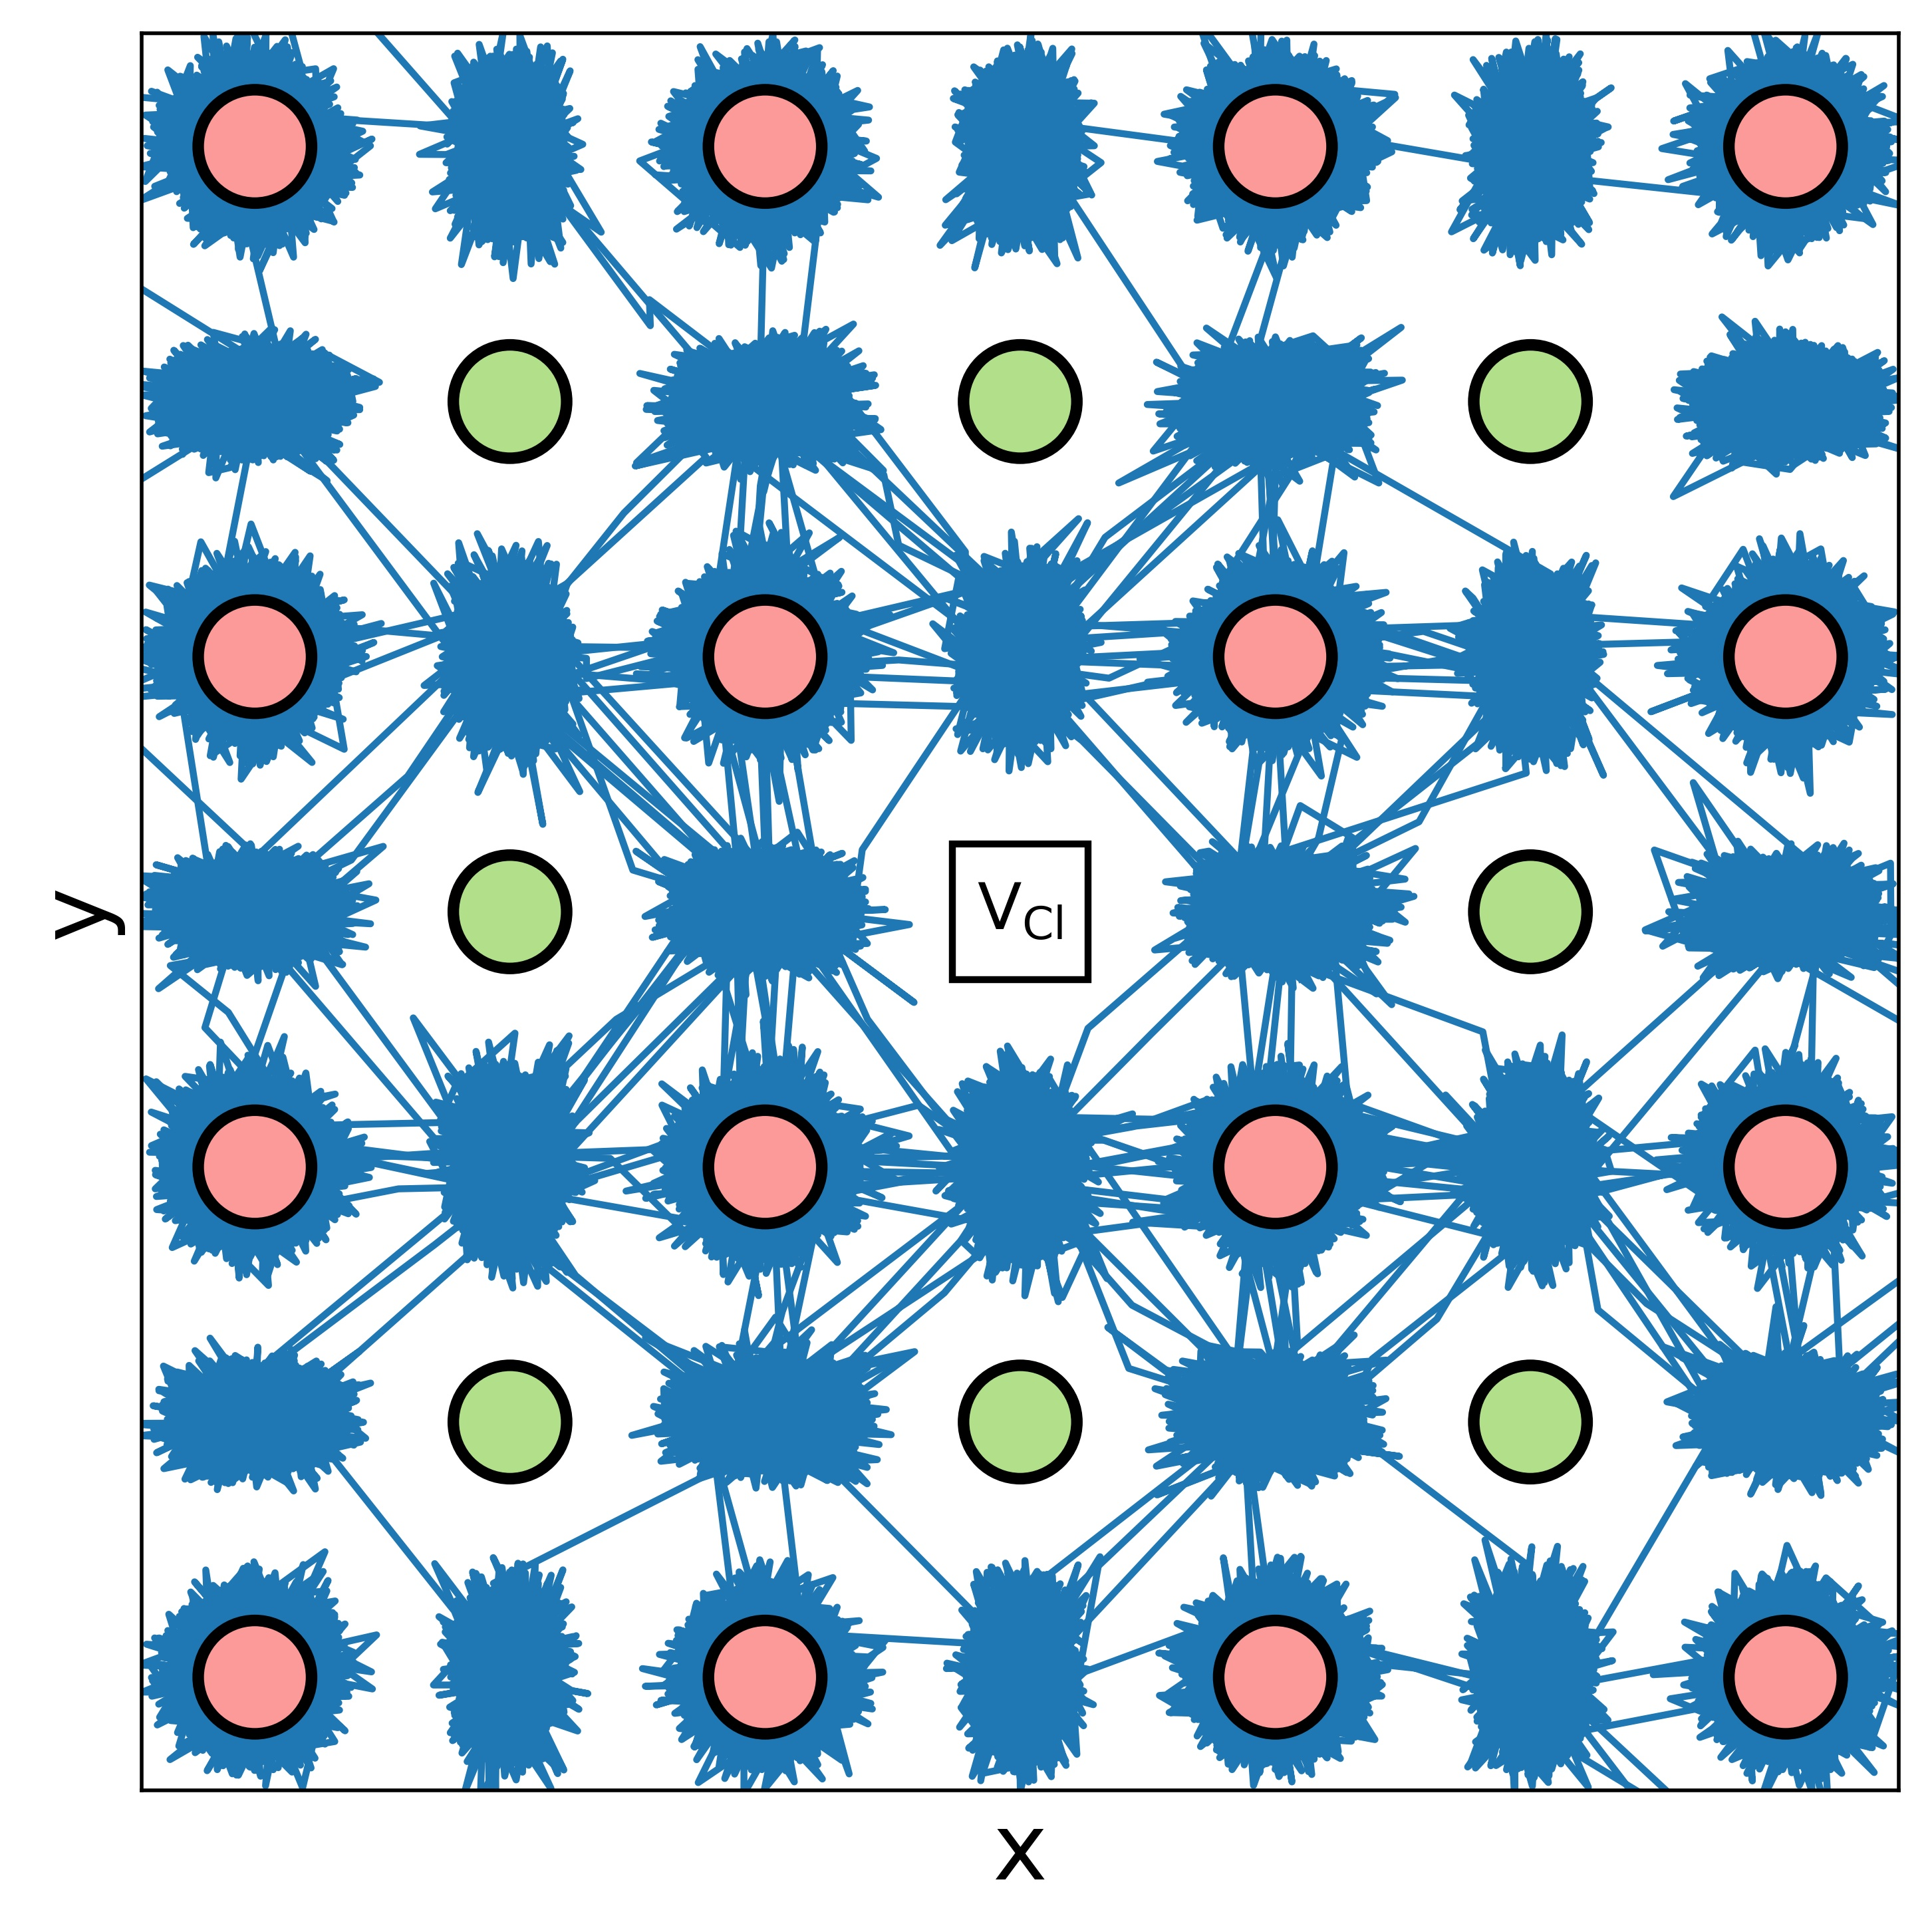
\includegraphics[width=5.6cm]{./figures/traj_centred_undoped.jpg}\label{undoped}}
    
    \sidesubfloat[]{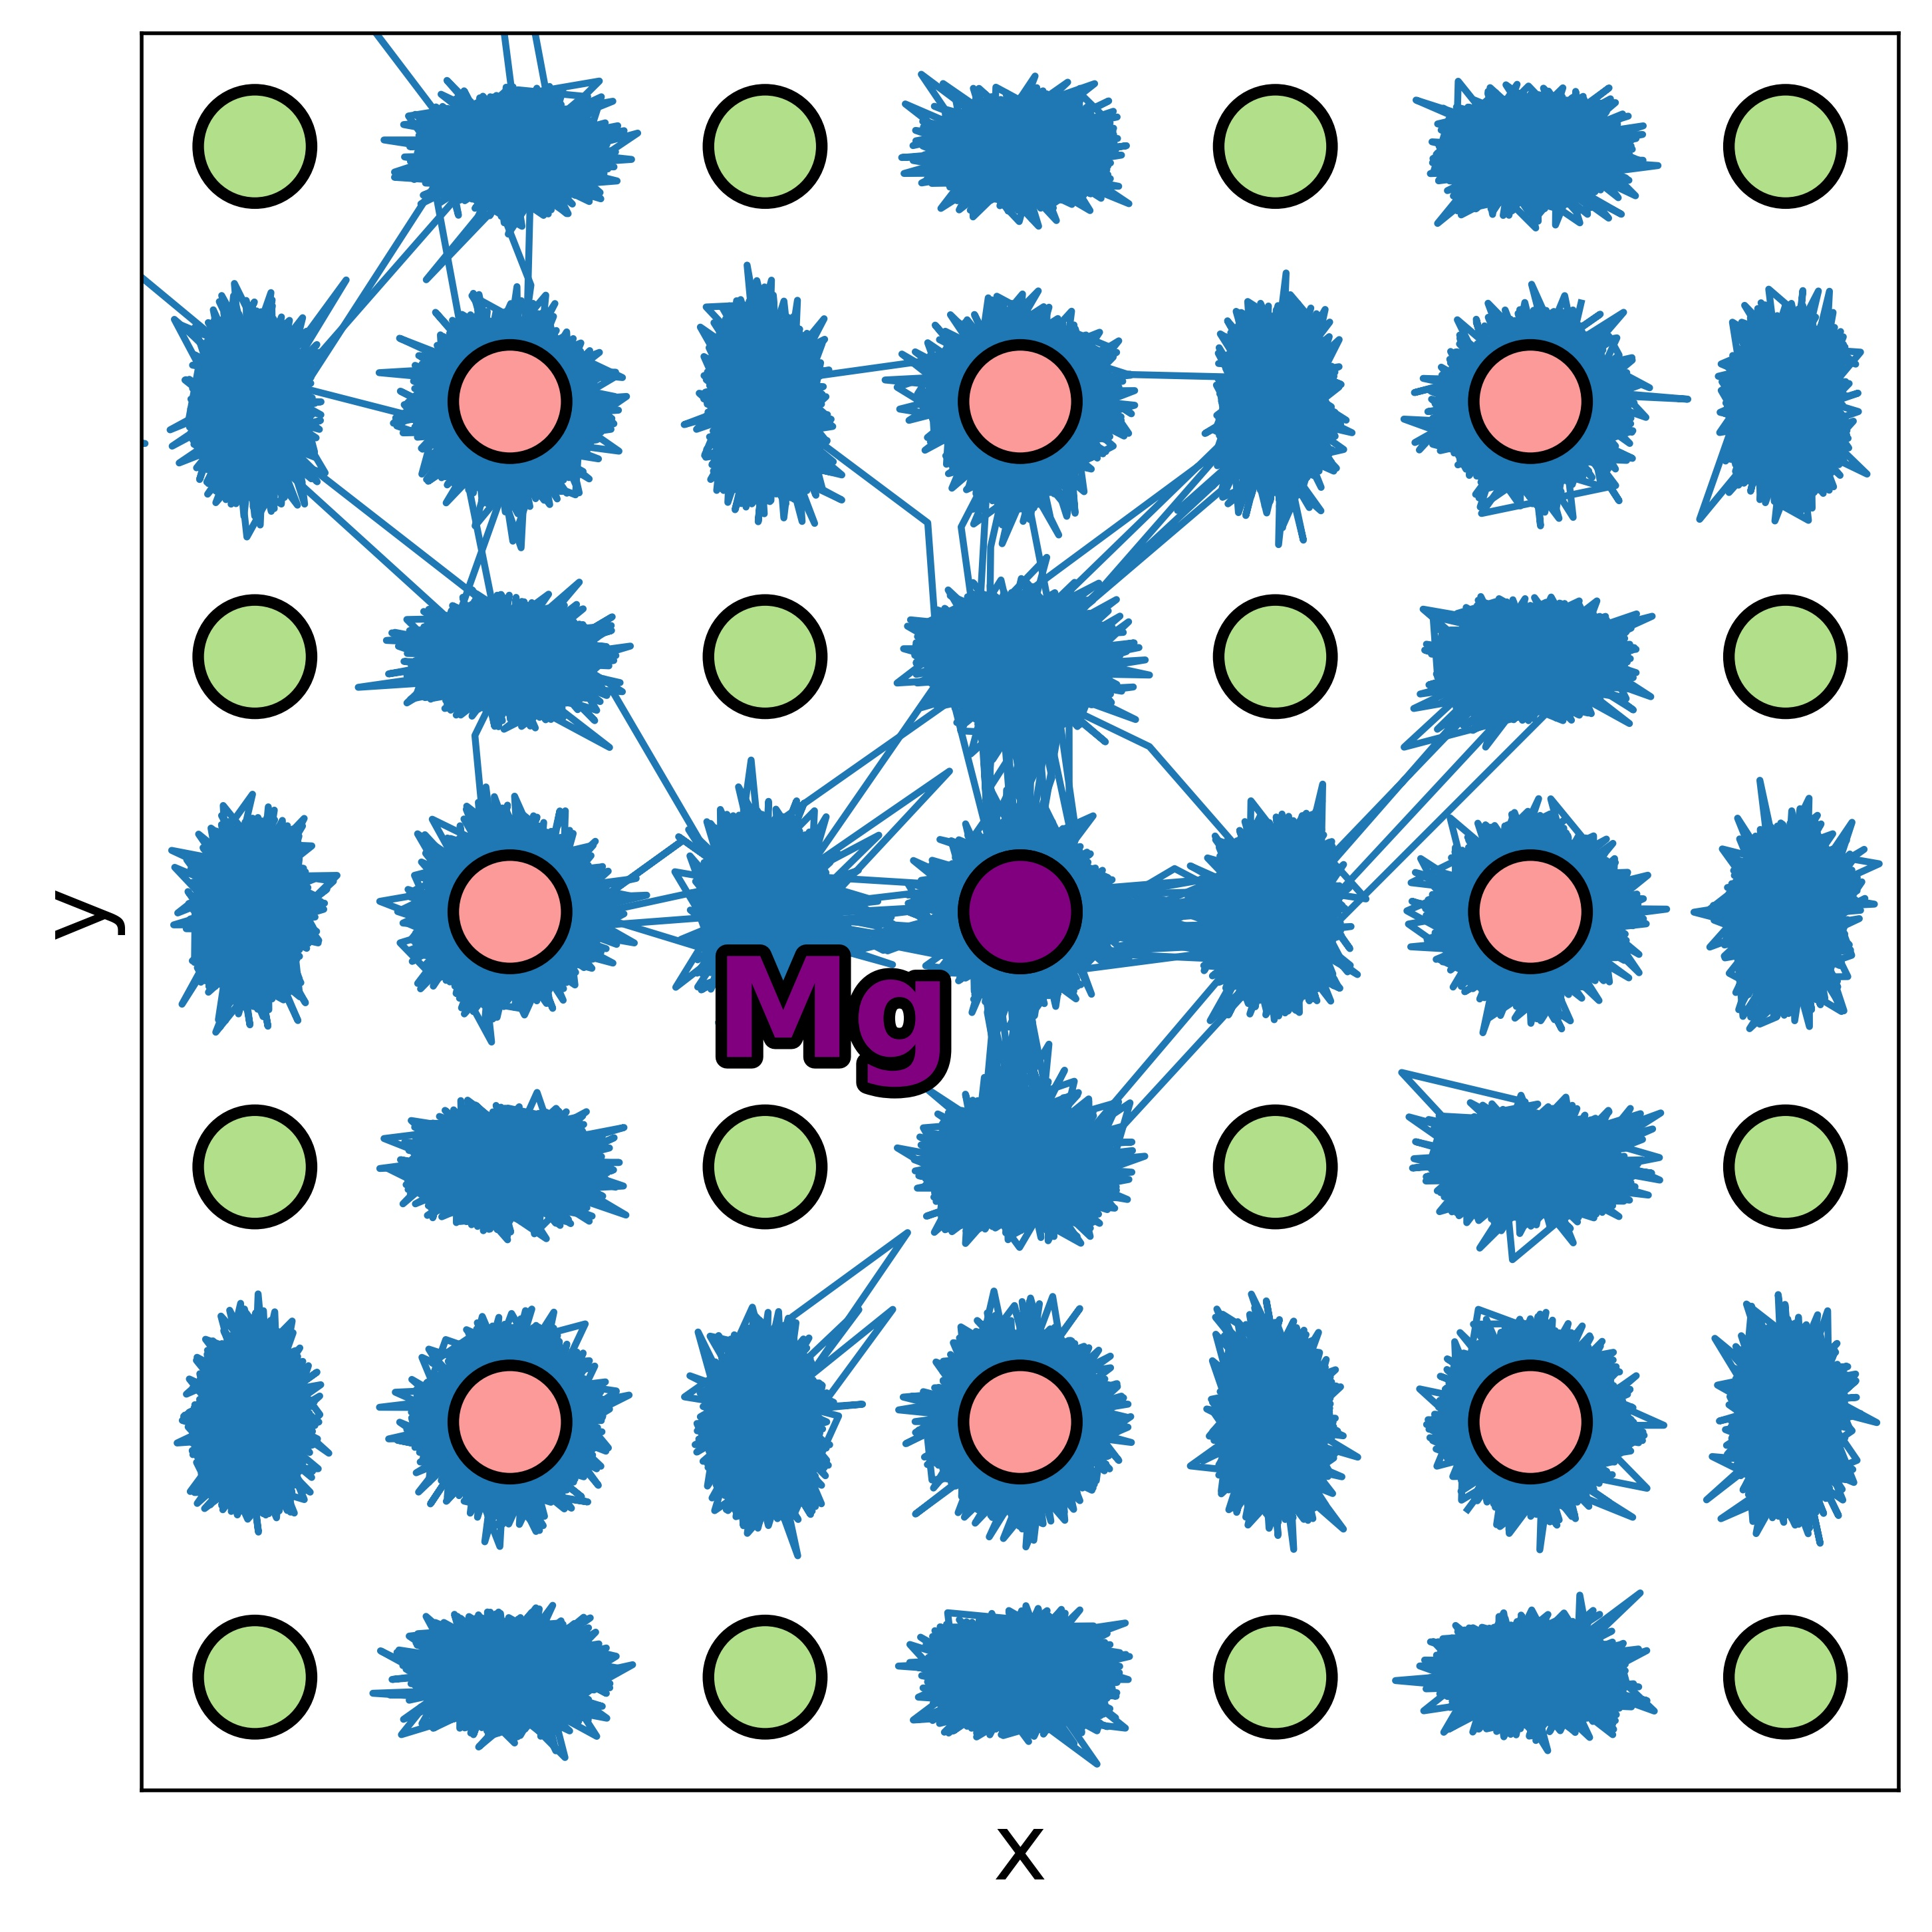
\includegraphics[width=5.6cm]{./figures/traj_centred_mg.jpg}\label{mg_doped}}
    
    \sidesubfloat[]{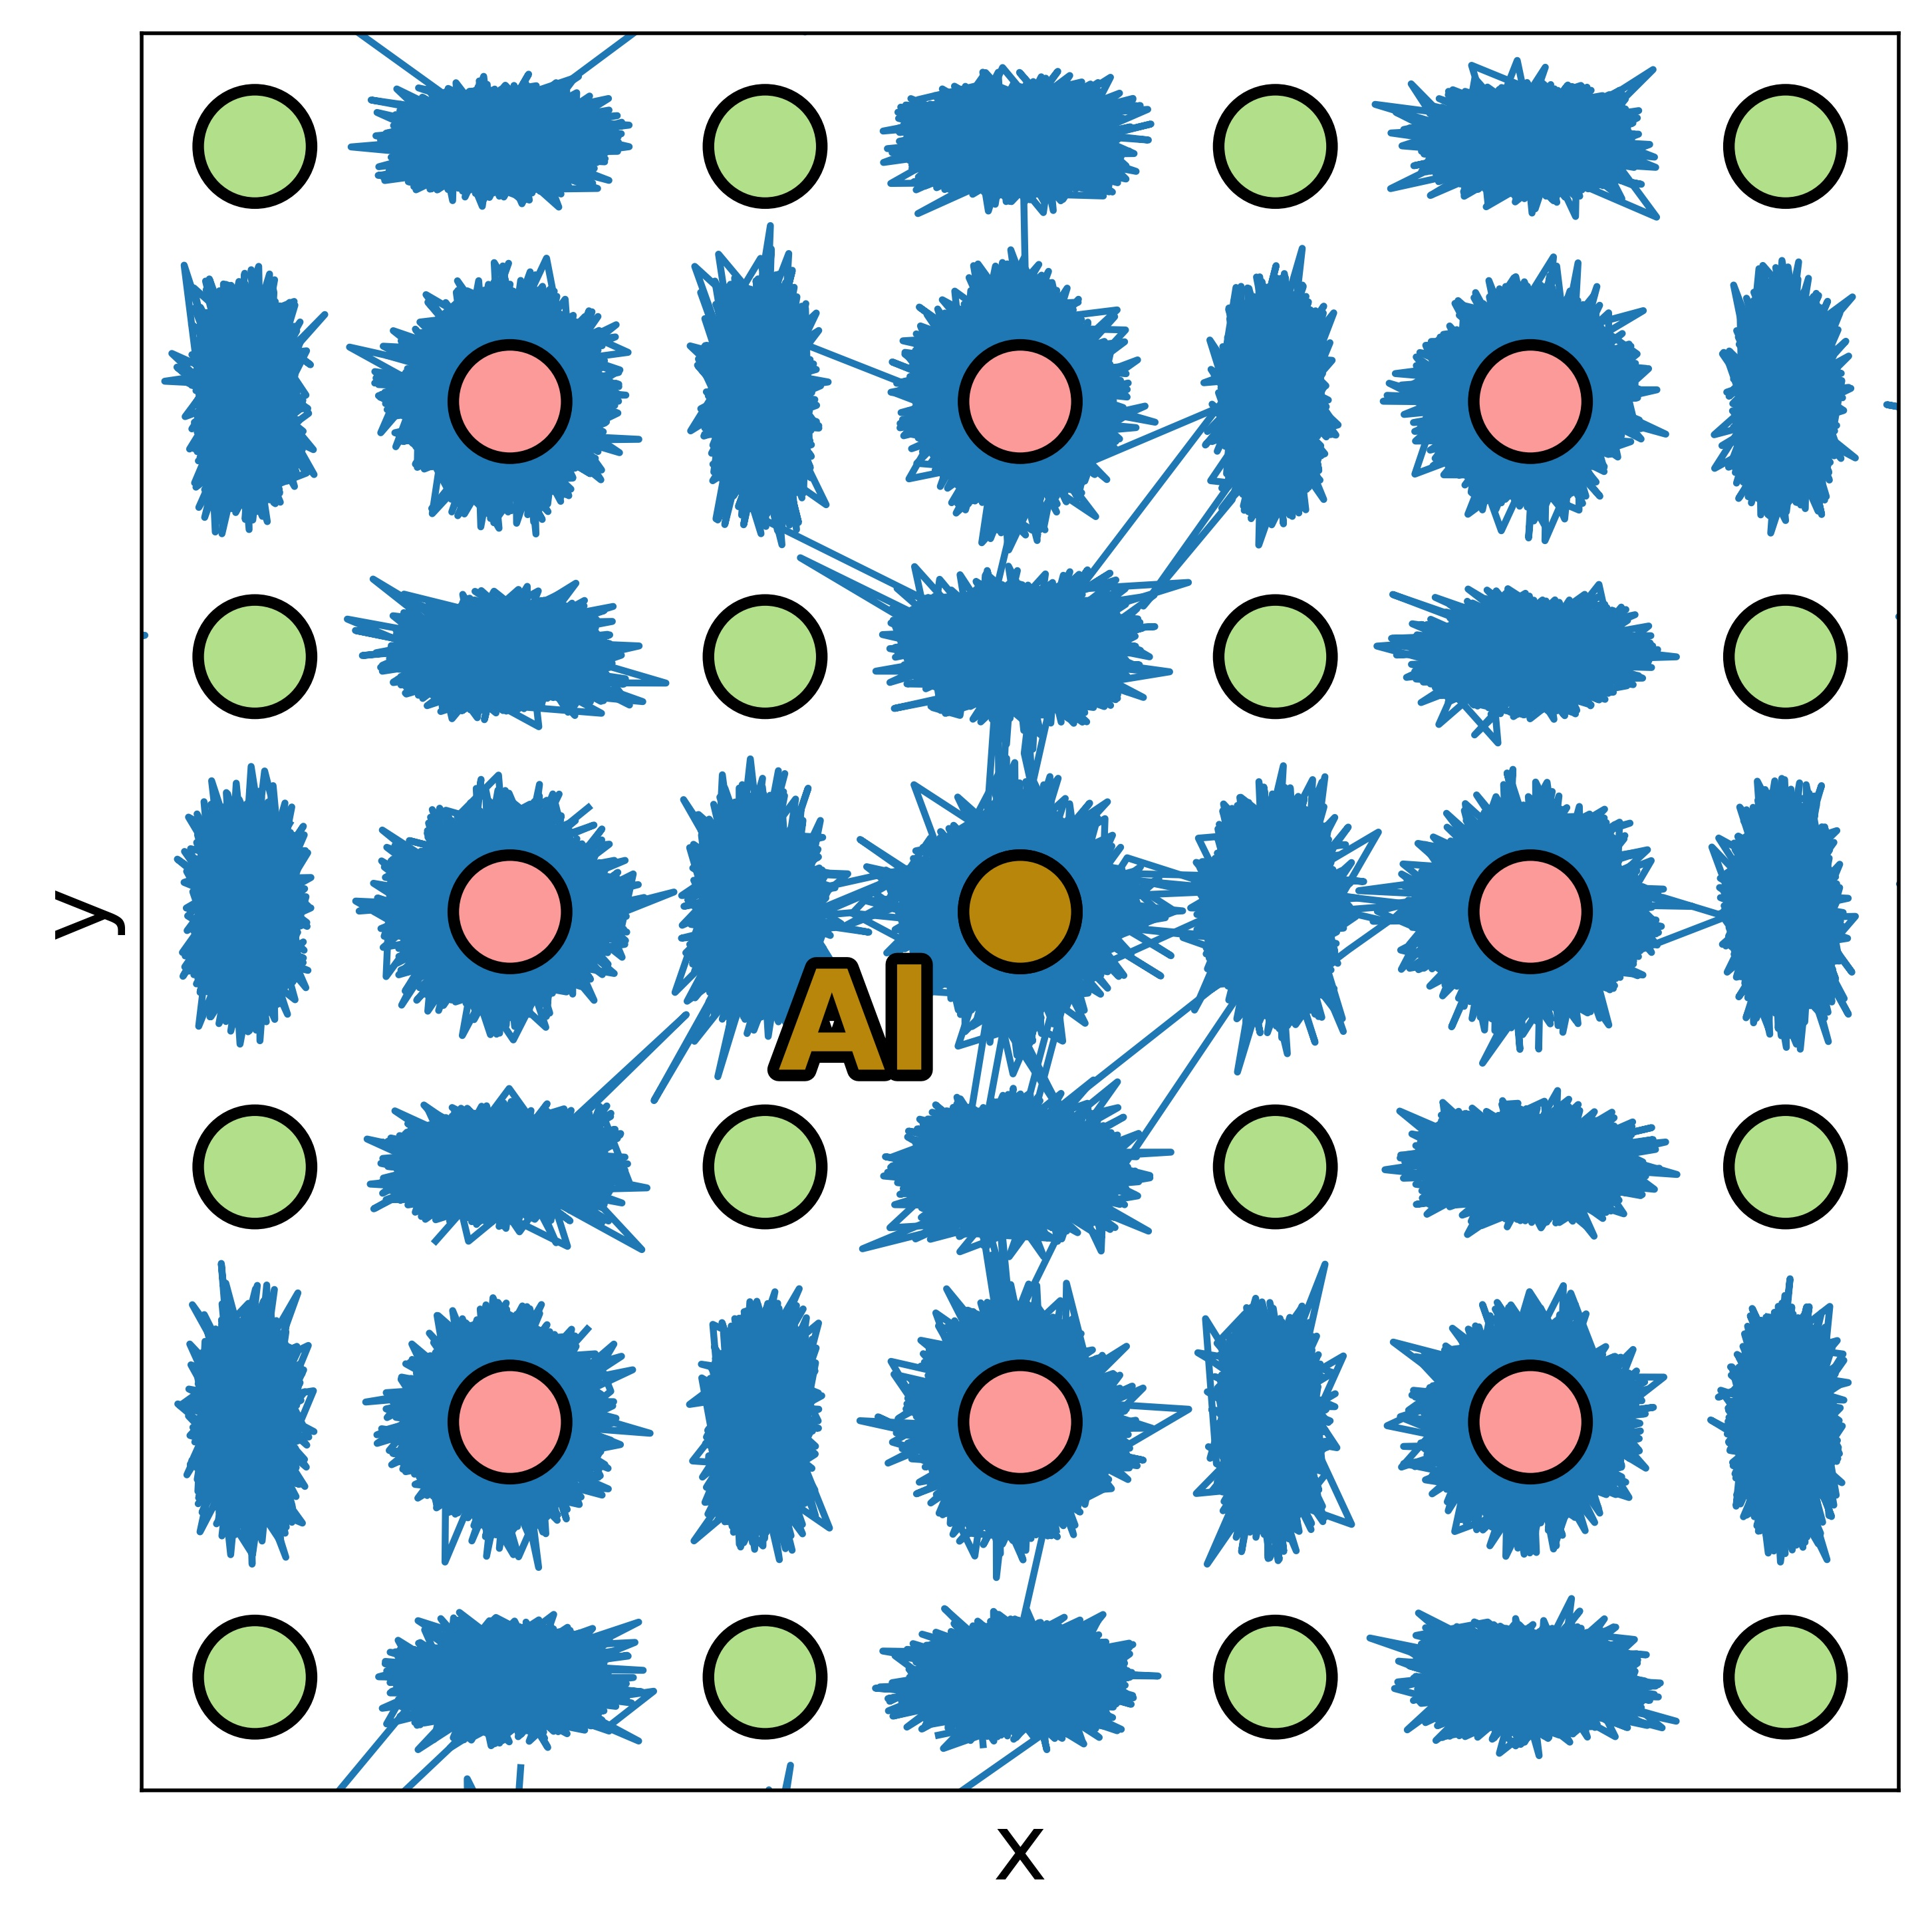
\includegraphics[width=5.6cm]{./figures/traj_centred_al.jpg}\label{al_doped}}
    
    \subfloat{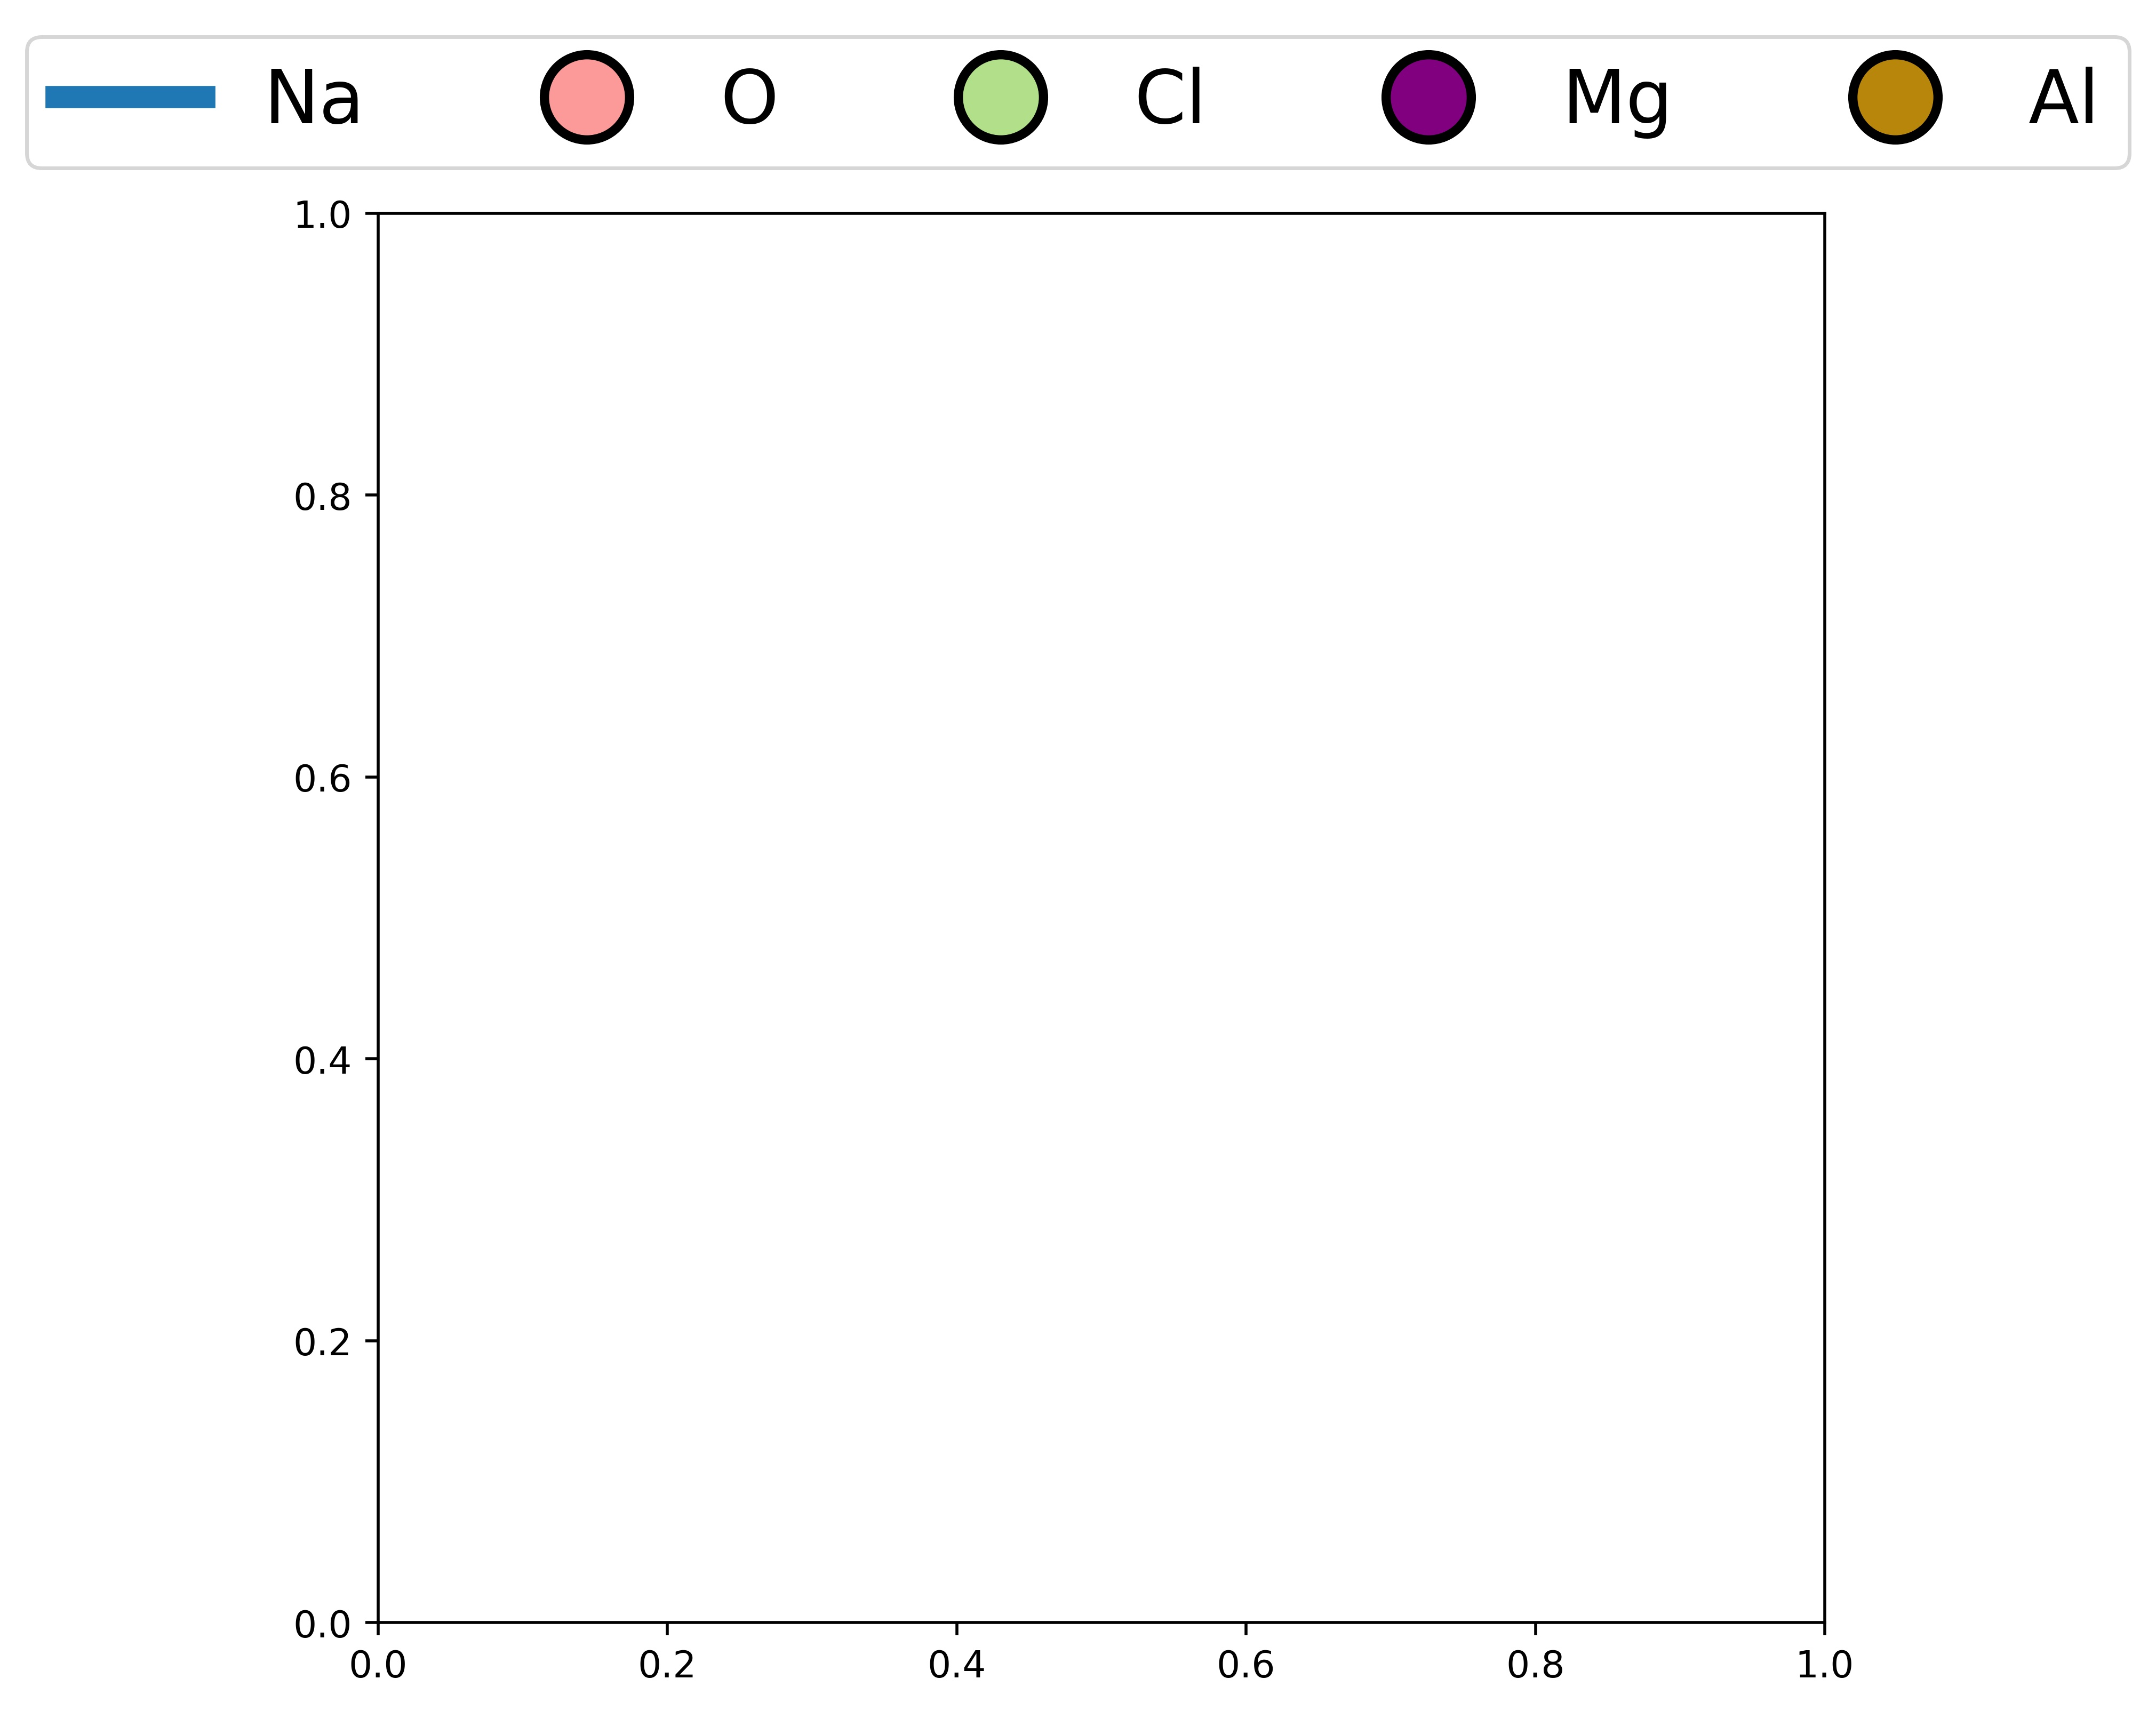
\includegraphics[width=8cm]{./figures/traj_centred_legend.jpg}\label{legend}}
\caption{Trajectory lines for Na-ion migration with a 0.27\% Na vacancy concentration (a) undoped system, (b) Mg-doped system and (c) Al-doped system. The first 2 ns and a 3x3x3 fraction of the supercell at 900 K are shown. O, Cl, Mg and Al ions are brought to the foreground for clarity, but it is important to note that not all of the ions occupy the same plane.}
\label{trajectories}
\end{figure}

Further insights into mechanistic features of Na-ion transport can be gained from visualising the ion jumps or line trajectories from the large-scale MD simulations (shown in Figure \ref{trajectories}); this illustrates the movement of Na-ions in the undoped structure and in the doped structures with the lowest (\ch{Mg^{2+}}) and highest (\ch{Al^{3+}}) binding energies. 
A relatively free migration of Na ions can be found in the undoped structure with ionic motion slightly inhibited in the doped structures, as depicted by greater Na ion densities close to the Mg and Al dopant ions; this effect is due to a degree of defect clustering predicted from our binding energy results, which would also lead to differences in Na-ion conductivity as found in Figure \ref{conductivity}. 
The line trajectories connecting Na sites also confirms that Na-ion migration takes place along the \ch{ONa6} octahedral edges. 

\section{Conclusions}

Atomic-scale insights into the transport behaviour of Na-ion solid electrolytes are important for the development of sodium-based solid-state batteries. 
In this study, we investigated the cation doping mechanisms and ionic conductivity in the anti-perovskite \ch{Na3OCl} by examining a wider range of aliovalent dopants than current experimental reports. 
Three main conclusions emerge.

(i) The observed structure is simulated accurately, and the lowest energy intrinsic defect is found to be the NaCl Schottky type, although its magnitude ($\mathrm{\sim}$2 eV) suggests a very small vacancy population in the undoped material. 

(ii) The most favourable aliovalent cation dopants are \ch{Mg^{2+}}, \ch{Ca^{2+}}, \ch{Al^{3+}} and \ch{Ga^{3+}} with Na-vacancy charge-compensation; an increase in Na vacancy concentration would promote Na-ion conductivity. 
The highest conductivity is found for the Mg-doped system of the order of $\mathrm{10^{-5} \ S \ cm^{-1}}$ at 500 K, but lower conductivities are predicted for the trivalent Al and Ga dopants. 
The migration profile and ion trajectory plots confirm 3D Na-ion conduction through curved pathways at the edges of the \ch{ONa6} octahedra. 

(iii) The defect binding energies suggest a high level of Na-vacancy/dopant clustering especially for the Ca, Al and Ga dopants, which would hinder Na-ion conduction.  
The smallest binding energy is found for the Mg dopant, which correlates with the higher conductivity for the Mg-doped system. 
We anticipate this study to stimulate further structural investigations of defect clusters at the microscopic level. 

The results presented here help to provide a framework to guide future doping studies on these anti-perovskite materials in order to optimize their properties for use as solid electrolytes in sodium-based solid-state batteries. 

\section{Future work}

(a) The effects of grain boundaries on the ionic conductivity of the Li-rich anti-perovskite \ch{Li3OCl} have been studied previously.\cite{dawson2018b, shen2020} 
However, these are still uncharacterised in the Na-rich analogue.
To investigate grain boundary effects in \ch{Na3OCl}, the low-energy grain boundaries in the structure must first be identified, by considering a range of possible variants.
Then, MD simulations can be run on these low-energy grain boundaries, to gain insight into how \ch{Na+} ions behave as they migrate across and within these grain boundaries.
Furthermore, dopant ions can also be introduced to the simulations, to explore dopant effects on the microscopic scale.

\begin{figure}[h]
    \centering
    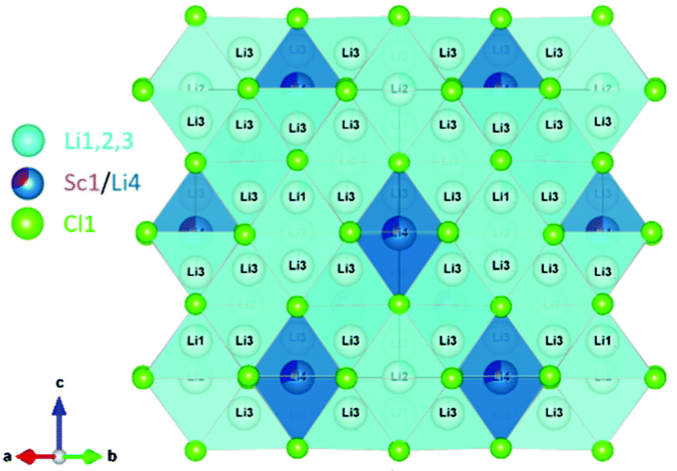
\includegraphics[width=10cm]{./figures/halo.png}
    \caption{Structure of the disordered halospinel \ch{Li2Sc_{2/3}Cl4} from TOF powder neutron diffraction. The blue \ch{(Sc/Li)Cl6} octahedral and green \ch{LiCl4} tetrahedral sites are all available to be occupied by Li.\cite{zhou2020}}
    \label{spinel}
\end{figure}

\noindent
(b) The investigation of other potential solid electrolyte materials is an additional area for future work.
Novel halide-based solid electrolytes have recently attracted attention due to their relatively high room temperature ionic conductivities in the $\mathrm{10^{-3} \ S \ cm^{-1}}$ range, as well as their wide electrochemical windows.
In particular, the disordered spinel, \ch{Li2Sc_{2/3}Cl4}, reported by Zhou \textit{et al.} in 2020 exhibits an ionic conductivity of $\mathrm{1.5 \times 10^{-3} \ S \ cm^{-1}}$, with a low activation energy for Li-ion diffusion of 0.34 eV.\cite{zhou2020}
Neutron diffraction studies on this material revealed that there is significant disorder in the Li-ion distribution over the energetically similar octahedral and tetrahedral sites in the spinel structure (Figure \ref{spinel}).
However, while experimental results on the material are promising, the atomic-scale effects that control ionic migration are still not clear.
Using potentials-based defect calculations and MD simulations, the underlying effects that result in the high ionic conductivity may be better understood and potentially further optimised.





\addcontentsline{toc}{chapter}{References}
\typeout{}
\bibliography{./refs/exportlist}
\bibliographystyle{./refs/rsc}


\clearpage





\appendix
\addappheadtotoc

\chapter{Defects}

\section{Point defects}

The three types of point defects relevant to this study are vacancies, interstitials and impurities.
Vacancies arise when ions move off their site to a point at an infinite distance away from the defect and leave an unfilled site.
The ion moving away leads to attractive interactions being broken, meaning vacancies are usually positive in energy.

Intersitials are ions that reside in sites unoccupied in the pristine lattice.
Unlike vacancies, the addition of an ion establishes attractive interactions, so interstitials tend to be negative in energy.
However, large interstitials can displace neighbouring ions, making the defect less favourable.

Finally, impurities are instances where a foreign ion is introduced into a perfect crystal.
These ions may occupy interstitial sites (interstitial impurities) or displace an ion of the crystal (substitutional impurities).
The energy of impurities can be either positive or negative depending on the ions involved.

\section{Kr\"oger-Vink notation}

The Kr\"oger-Vink notation is a useful tool to describe interactions involving defects.
Point defects are be represented by a simple shorthand of the form:

\begin{equation}
    i_{j}^{k}
\end{equation}

\noindent
Here, $i$ denotes the species in discussion, $j$ signifies the site occupied by the species, and $k$ shows the charge of the point defect. The possible values of $i$, $j$ and $k$ are presented in Table \ref{kv}.

\begin{table}[h]
\centering
\resizebox{\textwidth}{!}{%
\begin{tabular}{ c l l }
 \hline
 \textbf{Symbol} & \textbf{Possible Values} & \textbf{Explanation} \\ 
 \hline
 $i$ & H, Li, Be, ... & Atomic symbol of ion occupying the site. \\
  & V & Vacancy. \\
 $j$ & $\times$ & Neutral charge. \\
  & $\bullet$, $\bullet\bullet$, $\bullet\bullet\bullet$, ... & Positive charge of value 1+, 2+, 3+, etc. \\
  & $\prime$, $\prime\prime$, $\prime\prime\prime$, ... & Negative charge of value 1-, 2-, 3-, etc. \\
 $k$ & H, Li, Be, ... & Atomic symbol of ion occupying the site in the pristine crystal. \\
  & i & Interstitial site. \\
 \hline
\end{tabular}}
\caption{Details of the Kr\"oger-Vink notation system to describe point defects in crystal systems. }
\label{kv}
\end{table}

\noindent
For example, a vacancy on a sodium site would be described as:

\begin{equation}
    \mathrm{V_{Na}^{\prime}}
\end{equation}

\noindent
Further detail on the Kr\"oger-Vink notation used in this work is available in Table \ref{point_energies}.

\section{Intrinsic defects}

Ionic lattices at non-zero temperatures have thermal energy, which allows access to higher energy states, such as those containing defects.
The process of accessing these states is known as intrinsic defect formation.
Ionic lattices have varying levels of intrinsic defects depending on their formation energies.
The two types of intrinsic defects relevant for this study are Frenkel and Schottky defects.
When ions move off their lattice site into interstitial space it forms a Frenkel defect, described by the following equation for a monovalent ion A:

\begin{equation}
    \mathrm{A_A^{\times} \rightarrow V_A^{\bullet/\prime} + A_i^{\prime/\bullet}}
\end{equation}

\noindent
Schottky defects involve multiple species leaving their site in a concerted fashion with the formation of some new crystal.
The species leave vacancies behind, as described below for monovalent ions A and B:

\begin{equation}
    \mathrm{A_A^{\times} + B_B^{\times} \rightarrow V_A^{\bullet/\prime} + V_B^{\prime/\bullet} + AB}
\end{equation}

\noindent
The possible intrinsic defects in \ch{Na3OCl} and their formation energies are presented in Table \ref{def_e}.

\section{Migration mechanisms}

Perfect ionic crystals tend to be poor ionic conductors and the ionic transport in solid electrolytes often rely on the presence of defects in the lattice.
The most common modes of ionic transport in solid electrolytes are the interstitial and vacancy migration mechanisms.\cite{mehrer2007} 

When mobile interstitial ions are present in the lattice, the interstitial migration mechanism is likely to be dominant.
Interstitial ions may be present in undoped crystals if the Frenkel-type intrinsic defects are dominant.
This can be the case if small, low-valency ions are present, which have favourable vacancy and interstitial formation energies.
Interstitial defects may also be induced via aliovalent doping.

The second common mode of ionic transport is the vacancy mechanism, which is dominant when vacancies are present and hopping from a filled site to the vacancy has a low energy barrier.
Schottky defects can provide these vacancies where they are the dominant intrinsic defects, or aliovalent dopants can be used to induce them.





\chapter{Isolated point defect energies in \ch{Na3OCl}}

\begin{table}[h]
\centering

\begin{tabular}{ l | l | r }
 \hline
 \textbf{Point defect} & \textbf{KV.} & \textbf{E (eV)} \\ 
 \hline
 Na vacancy & \ch{V_{Na}^{$\prime$}} & 4.78 \\

 Na interstitial & \ch{Na_i^{$\bullet$}} & -2.21 \\

 O vacancy & \ch{V_{O}^{$\bullet\bullet$}} & 21.88 \\

 O interstitial & \ch{O_i^{$\prime\prime$}} & -14.24 \\

 Cl vacancy & \ch{V_{Cl}^{$\bullet$}} & 5.19 \\

 Cl interstitial & \ch{Cl_i^{$\prime$}} & -1.51 \\
 \hline
 Mg impurity & \ch{Mg_{Na}^{$\bullet$}} & -16.29 \\

 Ca impurity & \ch{Ca_{Na}^{$\bullet$}} & -11.19 \\

 Sr impurity & \ch{Sr_{Na}^{$\bullet$}} & -9.41 \\

 Ba impurity & \ch{Ba_{Na}^{$\bullet$}} & -7.32 \\

 Al impurity & \ch{Al_{Na}^{$\bullet\bullet$}} & -42.90 \\

 Ga impurity & \ch{Ga_{Na}^{$\bullet\bullet$}} & -39.76 \\
 \hline
 Cl vac. - Na vac. cluster & \ch{V_{Cl}^{$\bullet$}} - \ch{V_{Na}^{$\prime$}} & 9.64 \\

 Mg imp. - Na vac. cluster & \ch{Mg_{Na}^{$\bullet$}} - \ch{V_{Na}^{$\prime$}} & -11.82 \\

 Ca imp. - Na vac. cluster & \ch{Ca_{Na}^{$\bullet$}} - \ch{V_{Na}^{$\prime$}} & -6.98 \\

 Sr imp. - Na vac. cluster & \ch{Sr_{Na}^{$\bullet$}} - \ch{V_{Na}^{$\prime$}} & -5.20 \\

 Ba imp. - Na vac. cluster & \ch{Ba_{Na}^{$\bullet$}} - \ch{V_{Na}^{$\prime$}} & -3.17 \\

 Al imp. - Na vac. cluster & \ch{Al_{Na}^{$\bullet\bullet$}} - \ch{V_{Na}^{$\prime$}} & -38.87 \\

 Ga imp. - Na vac. cluster & \ch{Ga_{Na}^{$\bullet\bullet$}} - \ch{V_{Na}^{$\prime$}} & -35.65 \\
 \hline

\end{tabular}
\caption{Kr\"oger-Vink notations and defect energies for the investigated point defects in \ch{Na3OCl}.}
\label{point_energies}
\end{table}




\chapter{GULP dataset}

Example GULP dataset to find the energy of a Na vacancy in \ch{Na3OCl}.

\begin{Verbatim}[fontsize=\footnotesize]

opti conp comp defe
cell
4.504 4.504 4.504 90.0 90.0 90.0
frac
Cl core 0 0 0
O core 0.5 0.5 0.5
Cl shel 0 0 0
O shel 0.5 0.5 0.5
Na core 0.5 0.5 0
space
221
centre 0.5 0.5 0
vacancy 0.5 0.5 0
size 16 24
species
Na core 1.000
O core 0.183
O shel -2.183
Cl core 1.485
Cl shel -2.485
spring
O 593.716
Cl 29.3800
buckingham
Na core Na core 1788.19 0.159 0 0 12
Na core O shel 588.38 0.338 0 0 12
Na core Cl shel 1170.41 0.315 0 0 12
O shel O shel 22764.30 0.1490 13.19 0 12
O shel Cl shel 8286.91 0.2590 62.20 0 12
Cl shel Cl shel 1227.20 0.3210 14.53 0 12
dump Na3OCl.grs

\end{Verbatim}



\chapter{LAMMPS dataset}

Example LAMMPS dataset for a 10 ns MD run on a 16x16x16 supercell of the undoped \ch{Na3OCl} structure at 600 K.

\begin{Verbatim}[fontsize=\footnotesize]

# Input written to comply with LAMMPS 2017-08-11 00:00:00

# Atomic Configuration
units           metal
boundary        p p p
box tilt large
atom_style      charge
read_data       undoped.lmp
group           sodium type 1
group           oxide type 2
group           chloride type 3
variable        T1 equal 600

# Potential Setup
pair_style  buck/coul/long 12.0
pair_coeff * * 0.0 1.0 0.0
pair_coeff 1 1    1788.190000  0.159000   0.000000 # Na Na
pair_coeff 1 3    1170.410000  0.315000   0.000000 # Na Cl
pair_coeff 1 2     588.380000  0.338000   0.000000 # Na O 
pair_coeff 3 3    1227.200000  0.321000  14.530000 # Cl Cl
pair_coeff 2 3    8286.910000  0.259000  62.200000 # Cl O 
pair_coeff 2 2   22764.300000  0.149000  13.190000 # O  O 
kspace_style pppm 1e-05

# General Setup
timestep        0.001

# Thermodynamic Information Output
thermo_style custom step temp epair emol etotal press lx ly lz fmax cpu cpuremain
thermo          1000

# Intial Atom Velocity
velocity all create ${T1} 80800 dist gaussian rot yes

# Stage 0: npt_equilibriation
restart         0
fix             int all npt aniso 1.0 1.0 0.1 temp ${T1} ${T1} 0.5 
run             50000

# Stage 1: nvt_equilibriation
unfix int
restart         0
fix             int all nvt temp ${T1} ${T1} 0.5 
run             50000

# Stage 2: main_nvt_simulation
unfix int
compute         sodiummsd sodium msd com yes
compute         oxidemsd oxide msd com yes
compute         chloridemsd chloride msd com yes
fix             sodiummsdt sodium ave/time 1 1 1000 c_sodiummsd[4] \ 
                    file undoped_msd_na.txt
fix             oxidemymsdt oxide ave/time 1 1 1000 c_oxidemsd[4] \ 
                    file undoped_msd_o.txt
fix             chloridemymsdt chloride ave/time 1 1 1000 c_chloridemsd[4] \ 
                    file undoped_msd_cl.txt
dump            atom_info all custom 1000 undoped.lammpstrj \ 
                    element x y z q id type vx vy vz
dump_modify     atom_info append yes
dump_modify     atom_info sort id
dump_modify     atom_info element Na O Cl
restart         0
fix             int all nvt temp ${T1} ${T1} 0.5 
run             10000000

# Final Commands
variable final_energy equal etotal
print "final_energy: ${final_energy}"
print "END_OF_COMP"

\end{Verbatim}

\end{document}